\documentclass[a4paper]{book}
\usepackage{a4wide}
\usepackage{makeidx}
\usepackage{fancyhdr}
\usepackage{graphicx}
\usepackage{multicol}
\usepackage{float}
\usepackage{textcomp}
\usepackage{alltt}
\usepackage{times}
\usepackage{ifpdf}
\ifpdf
\usepackage[pdftex,
            pagebackref=true,
            colorlinks=true,
            linkcolor=blue,
            unicode
           ]{hyperref}
\else
\usepackage[ps2pdf,
            pagebackref=true,
            colorlinks=true,
            linkcolor=blue,
            unicode
           ]{hyperref}
\usepackage{pspicture}
\fi
\usepackage[utf8]{inputenc}
\usepackage{doxygen}
\makeindex
\setcounter{tocdepth}{3}
\renewcommand{\footrulewidth}{0.4pt}
\begin{document}
\begin{titlepage}
\vspace*{7cm}
\begin{center}
{\Large EOSKernel }\\
\vspace*{1cm}
{\large Generated by Doxygen 1.5.7}\\
\vspace*{0.5cm}
{\small Tue Sep 22 19:55:59 2009}\\
\end{center}
\end{titlepage}
\clearemptydoublepage
\pagenumbering{roman}
\tableofcontents
\clearemptydoublepage
\pagenumbering{arabic}
\chapter{Main Page}
\label{index}\hypertarget{index}{}EOS Kernel is the main software component of the EOS Framework. 
\chapter{Data Structure Index}
\section{Class Hierarchy}
This inheritance list is sorted roughly, but not completely, alphabetically:\begin{CompactList}
\item \contentsline{section}{EOSKernel}{\pageref{structEOSKernel}}{}
\item \contentsline{section}{EOSLuaEnvironment}{\pageref{classEOSLuaEnvironment}}{}
\item \contentsline{section}{EOSLuaScript}{\pageref{classEOSLuaScript}}{}
\begin{CompactList}
\item \contentsline{section}{EOSProcess}{\pageref{classEOSProcess}}{}
\end{CompactList}
\item \contentsline{section}{EOSLuaStackRestorer}{\pageref{classEOSLuaStackRestorer}}{}
\item \contentsline{section}{EOSLuaThisRestorer}{\pageref{classEOSLuaThisRestorer}}{}
\item \contentsline{section}{EOSMessage}{\pageref{classEOSMessage}}{}
\item \contentsline{section}{EOSScriptManager}{\pageref{classEOSScriptManager}}{}
\item \contentsline{section}{luaScriptBuffer}{\pageref{structluaScriptBuffer}}{}
\item \contentsline{section}{MessageField}{\pageref{classMessageField}}{}
\item \contentsline{section}{VariantData}{\pageref{classVariantData}}{}
\end{CompactList}

\chapter{Data Structure Index}
\section{Data Structures}
Here are the data structures with brief descriptions:\begin{CompactList}
\item\contentsline{section}{\hyperlink{structEOSKernel}{EOSKernel} (Main class of the EOS Kernel module )}{\pageref{structEOSKernel}}{}
\item\contentsline{section}{\hyperlink{classEOSLuaEnvironment}{EOSLuaEnvironment} (This class wraps the Lua interpreter environment instance )}{\pageref{classEOSLuaEnvironment}}{}
\item\contentsline{section}{\hyperlink{classEOSLuaScript}{EOSLuaScript} (This class represents a single EOS Lua source script )}{\pageref{classEOSLuaScript}}{}
\item\contentsline{section}{\hyperlink{classEOSLuaStackRestorer}{EOSLuaStackRestorer} (This class is used to keep Lua stack always in a consistent state {\em (based on code from Richard Shephard, published on CodeProject website: \href{http://www.codeproject.com/cpp/luaincpp.asp}{\tt http://www.codeproject.com/cpp/luaincpp.asp})\/} )}{\pageref{classEOSLuaStackRestorer}}{}
\item\contentsline{section}{\hyperlink{classEOSLuaThisRestorer}{EOSLuaThisRestorer} (This class is used to load the correct \char`\"{}this\char`\"{} reference each time the execution enters on a new script {\em (based on code from Richard Shephard, published on CodeProject website: \href{http://www.codeproject.com/cpp/luaincpp.asp}{\tt http://www.codeproject.com/cpp/luaincpp.asp})\/} )}{\pageref{classEOSLuaThisRestorer}}{}
\item\contentsline{section}{\hyperlink{classEOSMessage}{EOSMessage} (This class models the EOS Message Structure )}{\pageref{classEOSMessage}}{}
\item\contentsline{section}{\hyperlink{classEOSProcess}{EOSProcess} (Class used to model an EOS Process (a single script instance) )}{\pageref{classEOSProcess}}{}
\item\contentsline{section}{\hyperlink{classEOSScriptManager}{EOSScriptManager} (Class used to load and manage source scripts )}{\pageref{classEOSScriptManager}}{}
\item\contentsline{section}{\hyperlink{structluaScriptBuffer}{luaScriptBuffer} (Simple structure to hold a source script buffer in memory )}{\pageref{structluaScriptBuffer}}{}
\item\contentsline{section}{\hyperlink{classMessageField}{MessageField} (This class represents a single field of an EOS Message Structure )}{\pageref{classMessageField}}{}
\item\contentsline{section}{\hyperlink{classVariantData}{VariantData} (Class used to handle Lua Variant (boolean/numeric/string) data in EOS Kernel )}{\pageref{classVariantData}}{}
\end{CompactList}

\chapter{File Index}
\section{File List}
Here is a list of all files with brief descriptions:\begin{CompactList}
\item\contentsline{section}{\hyperlink{_8dep_8inc}{.dep.inc} }{\pageref{_8dep_8inc}}{}
\item\contentsline{section}{\hyperlink{EOSKernel_8cpp}{EOSKernel.cpp} }{\pageref{EOSKernel_8cpp}}{}
\item\contentsline{section}{\hyperlink{EOSKernel_8h}{EOSKernel.h} }{\pageref{EOSKernel_8h}}{}
\item\contentsline{section}{\hyperlink{EOSLauncher_8cpp}{EOSLauncher.cpp} }{\pageref{EOSLauncher_8cpp}}{}
\item\contentsline{section}{\hyperlink{EOSLuaEnvironment_8cpp}{EOSLuaEnvironment.cpp} }{\pageref{EOSLuaEnvironment_8cpp}}{}
\item\contentsline{section}{\hyperlink{EOSLuaEnvironment_8h}{EOSLuaEnvironment.h} }{\pageref{EOSLuaEnvironment_8h}}{}
\item\contentsline{section}{\hyperlink{EOSLuaScript_8cpp}{EOSLuaScript.cpp} }{\pageref{EOSLuaScript_8cpp}}{}
\item\contentsline{section}{\hyperlink{EOSLuaScript_8h}{EOSLuaScript.h} }{\pageref{EOSLuaScript_8h}}{}
\item\contentsline{section}{\hyperlink{EOSLuaStackRestorer_8h}{EOSLuaStackRestorer.h} }{\pageref{EOSLuaStackRestorer_8h}}{}
\item\contentsline{section}{\hyperlink{EOSLuaThisRestorer_8h}{EOSLuaThisRestorer.h} }{\pageref{EOSLuaThisRestorer_8h}}{}
\item\contentsline{section}{\hyperlink{EOSMessage_8cpp}{EOSMessage.cpp} }{\pageref{EOSMessage_8cpp}}{}
\item\contentsline{section}{\hyperlink{EOSMessage_8h}{EOSMessage.h} }{\pageref{EOSMessage_8h}}{}
\item\contentsline{section}{\hyperlink{EOSProcess_8cpp}{EOSProcess.cpp} }{\pageref{EOSProcess_8cpp}}{}
\item\contentsline{section}{\hyperlink{EOSProcess_8h}{EOSProcess.h} }{\pageref{EOSProcess_8h}}{}
\item\contentsline{section}{\hyperlink{EOSScriptManager_8cpp}{EOSScriptManager.cpp} }{\pageref{EOSScriptManager_8cpp}}{}
\item\contentsline{section}{\hyperlink{EOSScriptManager_8h}{EOSScriptManager.h} }{\pageref{EOSScriptManager_8h}}{}
\item\contentsline{section}{\hyperlink{VariantData_8h}{VariantData.h} }{\pageref{VariantData_8h}}{}
\end{CompactList}

\chapter{Data Structure Documentation}
\hypertarget{structEOSKernel}{
\section{EOSKernel Class Reference}
\label{structEOSKernel}\index{EOSKernel@{EOSKernel}}
}
Main class of the EOS Kernel module.  


{\tt \#include $<$EOSKernel.h$>$}

\subsection*{Public Member Functions}
\begin{CompactItemize}
\item 
\hyperlink{structEOSKernel_4d41f3d1f8081b9e9e729708ae66996b}{$\sim$EOSKernel} ()
\begin{CompactList}\small\item\em destructor \item\end{CompactList}\item 
void \hyperlink{structEOSKernel_6cbf49a8f46959908b08abaa969b0764}{start} (const char $\ast$appPath, bool norun)
\begin{CompactList}\small\item\em starts the kernel \item\end{CompactList}\item 
void \hyperlink{structEOSKernel_c0cf9a53338567326ad7e6388a54d208}{stop} ()
\begin{CompactList}\small\item\em stops the kernel \item\end{CompactList}\item 
\hyperlink{classEOSLuaEnvironment}{EOSLuaEnvironment} $\ast$ \hyperlink{structEOSKernel_dc571bb375ca531603c49e15bd5b5e1e}{getLuaEnvironment} ()
\begin{CompactList}\small\item\em returns a pointer to the current \hyperlink{classEOSLuaEnvironment}{EOSLuaEnvironment} wrapper class \item\end{CompactList}\end{CompactItemize}
\subsection*{Static Public Member Functions}
\begin{CompactItemize}
\item 
static \hyperlink{structEOSKernel}{EOSKernel} $\ast$ \hyperlink{structEOSKernel_b18f0db248717d197b3f0963265bf541}{getInstance} ()
\begin{CompactList}\small\item\em returns the static instance of the class \item\end{CompactList}\item 
static int \hyperlink{structEOSKernel_ed482eda9801f20453fdca40d91e7512}{moduleLoad} (lua\_\-State $\ast$luaRuntime)
\begin{CompactList}\small\item\em {\em (Lua binding interface: mapped to {\bf eos.module.load})\/}\par
\par
 Loads a module in EOS environment \item\end{CompactList}\item 
static int \hyperlink{structEOSKernel_5818cdf156babf931c7203339d6ee8ac}{shutdown} (lua\_\-State $\ast$luaRuntime)
\begin{CompactList}\small\item\em {\em (Lua binding interface: mapped to {\bf eos.shutdown})\/}\par
\par
 Shuts down the kernel (closes the application) \item\end{CompactList}\item 
static int \hyperlink{structEOSKernel_b1d4a0583d293c85eaec6d645aa073de}{sleep} (lua\_\-State $\ast$luaRuntime)
\begin{CompactList}\small\item\em {\em (Lua binding interface: mapped to {\bf eos.sleep})\/}\par
\par
 Suspends kernel execution for a given number of milliseconds \item\end{CompactList}\item 
static int \hyperlink{structEOSKernel_8b244f5fbf545937dccaa2cb01720f33}{getCurrentTime} (lua\_\-State $\ast$luaRuntime)
\begin{CompactList}\small\item\em {\em (Lua binding interface: mapped to {\bf eos.time.getCurrent})\/}\par
\par
 Returns the time (in seconds) since application started \item\end{CompactList}\item 
static int \hyperlink{structEOSKernel_3b68f7decae2685ffa3137f290656a1e}{getCurrentTimeMillis} (lua\_\-State $\ast$luaRuntime)
\begin{CompactList}\small\item\em {\em (Lua binding interface: mapped to {\bf eos.time.getCurrentMillis})\/}\par
\par
 Returns the time (in milliseconds) since application started \item\end{CompactList}\item 
static int \hyperlink{structEOSKernel_66a2b6a361992f0fb4c6e51c345e4811}{setTargetFrameRate} (lua\_\-State $\ast$luaRuntime)
\begin{CompactList}\small\item\em {\em (Lua binding interface: mapped to {\bf eos.setTargetFrameRate})\/}\par
\par
 Sets the target frame rate of the kernel (number of \char`\"{}update\char`\"{} executions per second) \item\end{CompactList}\item 
static int \hyperlink{structEOSKernel_38b029c0f4c889658b15b1fd87404934}{getTargetFrameRate} (lua\_\-State $\ast$luaRuntime)
\begin{CompactList}\small\item\em {\em (Lua binding interface: mapped to {\bf eos.getTargetFrameRate})\/}\par
\par
 Returns the current target frame rate of the kernel \item\end{CompactList}\item 
static int \hyperlink{structEOSKernel_d47c8cea2665110c5da64b2af16e49ac}{getLastFrameTime} (lua\_\-State $\ast$luaRuntime)
\begin{CompactList}\small\item\em {\em (Lua binding interface: mapped to {\bf eos.getLastFrameTime})\/}\par
\par
 Returns the duration (in seconds) of last kernel iteration (formerly a 'frame') \item\end{CompactList}\item 
static int \hyperlink{structEOSKernel_d1ccb01e71a53c8219f0d1a8a2fa87d1}{getApplicationRoot} (lua\_\-State $\ast$luaRuntime)
\item 
static int \hyperlink{structEOSKernel_e22b7cc7c59c6a3f40bbe3f45009b6f7}{processCreate} (lua\_\-State $\ast$luaRuntime)
\begin{CompactList}\small\item\em {\em (Lua binding interface: mapped to {\bf eos.process.create})\/}\par
\par
 Returns the time (in seconds) since application started \item\end{CompactList}\item 
static int \hyperlink{structEOSKernel_cd45fae422857bc7341451ff8b63f0aa}{processExists} (lua\_\-State $\ast$luaRuntime)
\begin{CompactList}\small\item\em {\em (Lua binding interface: mapped to {\bf eos.process.exists})\/}\par
\par
 Tests the existence of a process \item\end{CompactList}\item 
static int \hyperlink{structEOSKernel_4def28b41973ca584e9a701dc77493bc}{processSetActive} (lua\_\-State $\ast$luaRuntime)
\begin{CompactList}\small\item\em {\em (Lua binding interface: mapped to {\bf eos.process.setActive})\/}\par
\par
 Sets the activity status of a Process \item\end{CompactList}\item 
static int \hyperlink{structEOSKernel_0cc83428fafd6edbde079be3d40ab9b5}{processIsActive} (lua\_\-State $\ast$luaRuntime)
\begin{CompactList}\small\item\em {\em (Lua binding interface: mapped to {\bf eos.process.isActive})\/}\par
\par
 Sets the activity status of a Process \item\end{CompactList}\item 
static int \hyperlink{structEOSKernel_540af533e83f0920b55b4ad638a76ab5}{processDestroy} (lua\_\-State $\ast$luaRuntime)
\begin{CompactList}\small\item\em {\em (Lua binding interface: mapped to {\bf eos.process.destroy})\/}\par
\par
 Destroys a Process \item\end{CompactList}\item 
static int \hyperlink{structEOSKernel_b4212bfe6463d4d660724b74fa23fcca}{messageInit} (lua\_\-State $\ast$luaRuntime)
\begin{CompactList}\small\item\em {\em (Lua binding interface: mapped to {\bf eos.message.init})\/}\par
\par
 Initializes a message structure \item\end{CompactList}\item 
static int \hyperlink{structEOSKernel_a41c8c1590f49342c901ac8e0c055e2c}{messagePushData} (lua\_\-State $\ast$luaRuntime)
\begin{CompactList}\small\item\em {\em (Lua binding interface: mapped to {\bf eos.message.pushData})\/}\par
\par
 Pushes a data pair (key, value) in a previously initialized message (see messageInit) \item\end{CompactList}\item 
static int \hyperlink{structEOSKernel_3d3c99f27856467254fdbc66388e059f}{messageSend} (lua\_\-State $\ast$luaRuntime)
\begin{CompactList}\small\item\em {\em (Lua binding interface: mapped to {\bf eos.message.send})\/}\par
\par
 Sends a previously initialized and prepared message \item\end{CompactList}\item 
static int \hyperlink{structEOSKernel_32cd671874726365523a0ed8f0d21339}{setConsoleLogLevel} (lua\_\-State $\ast$luaRuntime)
\begin{CompactList}\small\item\em {\em (Lua binding interface: mapped to {\bf eos.log.setConsoleLogLevel})\/}\par
\par
 Sets the verbosity level (on stderr) of the EOS Kernel \item\end{CompactList}\item 
static int \hyperlink{structEOSKernel_9d25589438c403f7b8db9c77bb354a0c}{traceError} (lua\_\-State $\ast$luaRuntime)
\begin{CompactList}\small\item\em {\em (Lua binding interface: mapped to {\bf eos.log.traceError})\/}\par
\par
 Writes a line in eos.log logfile, with 'error' class mark (\mbox{[}E\mbox{]}) \item\end{CompactList}\item 
static int \hyperlink{structEOSKernel_186131b875c0871e4b0e5d4f9a484b16}{traceWarning} (lua\_\-State $\ast$luaRuntime)
\begin{CompactList}\small\item\em {\em (Lua binding interface: mapped to {\bf eos.log.traceWarning})\/}\par
\par
 Writes a line in EOS.log logfile, with 'warning' class mark (\mbox{[}W\mbox{]}) \item\end{CompactList}\item 
static int \hyperlink{structEOSKernel_3407dd17642df22065837296f2a49f8a}{traceDebug} (lua\_\-State $\ast$luaRuntime)
\begin{CompactList}\small\item\em {\em (Lua binding interface: mapped to {\bf eos.log.traceDebug})\/}\par
\par
 Writes a line in EOS.log logfile, with 'debug' class mark (\mbox{[}D\mbox{]}) \item\end{CompactList}\item 
static int \hyperlink{structEOSKernel_29224ae2d81261b6f4d859f6dfcde468}{traceUser} (lua\_\-State $\ast$luaRuntime)
\begin{CompactList}\small\item\em {\em (Lua binding interface: mapped to {\bf eos.log.traceUser})\/}\par
\par
 Writes a line in EOS.log logfile, with 'user' class mark (\mbox{[}U\mbox{]}) \item\end{CompactList}\item 
static int \hyperlink{structEOSKernel_dfbb944ca4916e758c9e3ada4c3f3644}{traceInfo} (lua\_\-State $\ast$luaRuntime)
\begin{CompactList}\small\item\em {\em (Lua binding interface: mapped to {\bf eos.log.traceInfo})\/}\par
\par
 Writes a line in EOS.log logfile, with 'info' class mark (\mbox{[}I\mbox{]}) \item\end{CompactList}\end{CompactItemize}
\subsection*{Data Fields}
\begin{CompactItemize}
\item 
int \hyperlink{structEOSKernel_834ee3631c926c273cb99ab2a80e2a4c}{consoleVerbosityLevel}
\begin{CompactList}\small\item\em verbosity level for the console (stderr) output \item\end{CompactList}\end{CompactItemize}
\subsection*{Static Public Attributes}
\begin{CompactItemize}
\item 
static int \hyperlink{structEOSKernel_c952db283e29f0b6927b130da6396d20}{SAFEGUARD\_\-ACTIVE} = 1
\begin{CompactList}\small\item\em safeguard mechanism: activity flag \item\end{CompactList}\item 
static int \hyperlink{structEOSKernel_c97927724be5b7c2eebf92739155ca0d}{SAFEGUARD\_\-FLAG\_\-LOADMODULE} = 2
\begin{CompactList}\small\item\em safeguard mechanism: module load check \item\end{CompactList}\item 
static struct luaL\_\-reg \hyperlink{structEOSKernel_b6b80a3e788ce2d8efcfc693d1e2e24c}{lua\_\-eoskernel\_\-main} \mbox{[}$\,$\mbox{]}
\begin{CompactList}\small\item\em contains top level lua binding functions (eos.$\ast$) \item\end{CompactList}\item 
static struct luaL\_\-reg \hyperlink{structEOSKernel_369f2e0709ea1be66f5f47dd5e861025}{lua\_\-eoskernel\_\-module} \mbox{[}$\,$\mbox{]}
\begin{CompactList}\small\item\em contains module handling lua binding functions (eos.module.$\ast$) \item\end{CompactList}\item 
static struct luaL\_\-reg \hyperlink{structEOSKernel_ffcec7d380b132f1dbebfd46b83f5c8d}{lua\_\-eoskernel\_\-time} \mbox{[}$\,$\mbox{]}
\begin{CompactList}\small\item\em contains time related lua binding functions (eos.time.$\ast$) \item\end{CompactList}\item 
static struct luaL\_\-reg \hyperlink{structEOSKernel_077213f420729c5a87f04c29fd14ce21}{lua\_\-eoskernel\_\-process} \mbox{[}$\,$\mbox{]}
\begin{CompactList}\small\item\em contains process handling lua binding functions (eos.process.$\ast$) \item\end{CompactList}\item 
static struct luaL\_\-reg \hyperlink{structEOSKernel_7033fb8fd34a75b851d9d9958e38c8f1}{lua\_\-eoskernel\_\-message} \mbox{[}$\,$\mbox{]}
\begin{CompactList}\small\item\em contains message handling lua binding functions (eos.message.$\ast$) \item\end{CompactList}\item 
static struct luaL\_\-reg \hyperlink{structEOSKernel_ed8c742384718b2e595d4f800178f80a}{lua\_\-eoskernel\_\-log} \mbox{[}$\,$\mbox{]}
\begin{CompactList}\small\item\em contains log handling lua binding functions (eos.log.$\ast$) \item\end{CompactList}\end{CompactItemize}
\subsection*{Private Member Functions}
\begin{CompactItemize}
\item 
\hyperlink{structEOSKernel_06b0f1294a41e6203f303991ccfd9f56}{EOSKernel} ()
\begin{CompactList}\small\item\em private constructor \item\end{CompactList}\item 
int \hyperlink{structEOSKernel_04741bac06a4289eeaa252290c9ea48f}{init} (const char $\ast$appPath, bool norun)
\begin{CompactList}\small\item\em runs early initialization code of the kernel \item\end{CompactList}\item 
int \hyperlink{structEOSKernel_d6091282d486d45fe2c243510031ad32}{makeScripts} (const char $\ast$scriptsPath)
\begin{CompactList}\small\item\em compiles given application source scripts \item\end{CompactList}\item 
bool \hyperlink{structEOSKernel_13844b7aae15bf38e0ceca3a5be52b9b}{safeguardCheck} ()
\begin{CompactList}\small\item\em safeguard mechanism: exception check \item\end{CompactList}\item 
void \hyperlink{structEOSKernel_29d304241dfe47c34d782b0b93a6b986}{update} ()
\begin{CompactList}\small\item\em executes an update cycle of the kernel (formerly a \char`\"{}frame\char`\"{}) \item\end{CompactList}\item 
void \hyperlink{structEOSKernel_2659cec44279505b550ab273010cb6b9}{run} ()
\begin{CompactList}\small\item\em starts kernel execution cycle \item\end{CompactList}\item 
void \hyperlink{structEOSKernel_c951ed12c4318cb8272849abf124ee51}{pause} (unsigned int milliseconds)
\begin{CompactList}\small\item\em pauses kernel for a given number of milliseconds \item\end{CompactList}\item 
void \hyperlink{structEOSKernel_f9ca04a44a732ba92ff65927f3757ffd}{cleanup} ()
\begin{CompactList}\small\item\em kernel resources cleanup. This function also calls cleanup on all loaded extension modules. \item\end{CompactList}\item 
bool \hyperlink{structEOSKernel_a58308c8aa2b19378d24af1cb51b78d2}{createProcess} (const char $\ast$processName, const char $\ast$scriptName)
\begin{CompactList}\small\item\em creates an EOS Process \item\end{CompactList}\item 
\hyperlink{classEOSProcess}{EOSProcess} $\ast$ \hyperlink{structEOSKernel_9b9fa8938a1ad005b3b55df2aa4ba32c}{processByName} (const char $\ast$processName)
\begin{CompactList}\small\item\em returns the pointer to an EOS Process, by its name \item\end{CompactList}\item 
bool \hyperlink{structEOSKernel_9ab346976e19d85ebfbad260b3913734}{setProcessActivity} (const char $\ast$processName, bool activity)
\begin{CompactList}\small\item\em sets the activity status of an EOS Process \item\end{CompactList}\item 
bool \hyperlink{structEOSKernel_214499b9e8c0ab67eddd377a780cb3fa}{destroyProcess} (const char $\ast$processName)
\begin{CompactList}\small\item\em destroys an EOS Process \item\end{CompactList}\item 
void \hyperlink{structEOSKernel_4b51e69b7ddd8e0fa02a339dfb5f86f9}{\_\-setFrameRate} (const char $\ast$requestedFrameRate)
\begin{CompactList}\small\item\em sets the target execution frame rate of the kernel \item\end{CompactList}\item 
float \hyperlink{structEOSKernel_68610ced573efe86f7db3ca176590793}{currentTime} ()
\begin{CompactList}\small\item\em returns elapsed time since kernel start, in seconds \item\end{CompactList}\item 
unsigned long \hyperlink{structEOSKernel_2b1e8769e99c2af88e199534c1cc694b}{currentTimeMillis} ()
\begin{CompactList}\small\item\em returns elapsed time since kernel start, in milliseconds \item\end{CompactList}\item 
void \hyperlink{structEOSKernel_3901b7994589931f6d409a3a7f42dae2}{logMessage} (int level, const char $\ast$format\_\-string,...)
\begin{CompactList}\small\item\em writes a line in the application log file \item\end{CompactList}\item 
void \hyperlink{structEOSKernel_5a647f0ff07643959bebac4408d6c105}{prepareMessage} (const char $\ast$messageClass)
\begin{CompactList}\small\item\em prepares (initializes) a new \hyperlink{classEOSMessage}{EOSMessage} structure \item\end{CompactList}\item 
void \hyperlink{structEOSKernel_335409b15526d516a8051199cc7fa619}{pushMessageData} (const char $\ast$messageDataKey, bool messageDataValue)
\begin{CompactList}\small\item\em pushes a boolean data field in the current \hyperlink{classEOSMessage}{EOSMessage} structure \item\end{CompactList}\item 
void \hyperlink{structEOSKernel_756f0c37601b7a9bc59832948a2b20ad}{pushMessageData} (const char $\ast$messageDataKey, float messageDataValue)
\begin{CompactList}\small\item\em pushes a numeric data field in the current \hyperlink{classEOSMessage}{EOSMessage} structure \item\end{CompactList}\item 
void \hyperlink{structEOSKernel_3e7745d89db284ffa185b399a88ff8e5}{pushMessageData} (const char $\ast$messageDataKey, const char $\ast$messageDataValue)
\begin{CompactList}\small\item\em pushes a string data field in the current \hyperlink{classEOSMessage}{EOSMessage} structure \item\end{CompactList}\item 
void \hyperlink{structEOSKernel_f515d2bca73d1c3eed643605274bc3c2}{sendPreparedMessage} (const char $\ast$messageReceiver)
\begin{CompactList}\small\item\em sends current \hyperlink{classEOSMessage}{EOSMessage} structure to the receiver Process \item\end{CompactList}\item 
void \hyperlink{structEOSKernel_9d3dac36c51293a2d55b5ccd55411fe1}{registerNativeLuaFunctions} ()
\end{CompactItemize}
\subsection*{Private Attributes}
\begin{CompactItemize}
\item 
EOSPrecisionTimer $\ast$ \hyperlink{structEOSKernel_cf859572d0066a9f3b14276c39d33845}{kernelTimer}
\begin{CompactList}\small\item\em precision timer to handle execution timings \item\end{CompactList}\item 
\hyperlink{classEOSLuaEnvironment}{EOSLuaEnvironment} $\ast$ \hyperlink{structEOSKernel_5b6a6d064e015c2db02ed67ca224f080}{luaEnvironment}
\begin{CompactList}\small\item\em instance of the class that manages Lua Runtime Environment \item\end{CompactList}\item 
\hyperlink{classEOSScriptManager}{EOSScriptManager} $\ast$ \hyperlink{structEOSKernel_b48245e1274b86370aebc583430b9199}{scriptManager}
\begin{CompactList}\small\item\em instance of the class that manages source scripts \item\end{CompactList}\item 
\hyperlink{classEOSProcess}{EOSProcess} $\ast$ \hyperlink{structEOSKernel_7224243c464c099b92494f3a06eeb99e}{masterProcess}
\begin{CompactList}\small\item\em pointer to the application's main process (MasterProcess is the only process automatically instanced by the kernel) \item\end{CompactList}\item 
\hyperlink{classEOSMessage}{EOSMessage} $\ast$ \hyperlink{structEOSKernel_a755627acbc4b4b61d4fcbdef216baef}{temporaryMessage}
\begin{CompactList}\small\item\em pointer to the temporary \hyperlink{classEOSMessage}{EOSMessage} structure \item\end{CompactList}\item 
std::queue$<$ \hyperlink{classEOSMessage}{EOSMessage} $\ast$ $>$ \hyperlink{structEOSKernel_e6cc8ecb01686b6284ec7fb8ce2d376f}{messageQueue}
\begin{CompactList}\small\item\em message queue \item\end{CompactList}\item 
unsigned long \hyperlink{structEOSKernel_200122496966050fd49e27dd74323093}{frameStart}
\item 
unsigned long \hyperlink{structEOSKernel_288bf0407fc19109c67102df51a4774c}{lastFrameTime}
\item 
unsigned long \hyperlink{structEOSKernel_96244c5052baeb3cb4915e655a12b50d}{targetFrameTime}
\begin{CompactList}\small\item\em fields used for timing purposes \item\end{CompactList}\item 
std::map$<$ std::string, \hyperlink{classEOSProcess}{EOSProcess} $\ast$ $>$ \hyperlink{structEOSKernel_2ef28158d540dabd63d2020e082fa925}{processes}
\begin{CompactList}\small\item\em processes hashmap \item\end{CompactList}\item 
unsigned int \hyperlink{structEOSKernel_1624f33c49b9fcdd0a0b4a8bd2342267}{safeguardRegistry}
\begin{CompactList}\small\item\em safeguard mechanism: flag registry \item\end{CompactList}\end{CompactItemize}
\subsection*{Static Private Attributes}
\begin{CompactItemize}
\item 
static bool \hyperlink{structEOSKernel_73cfb100d6374fd4cd0f5a7e80179b06}{instanceFlag} = false
\begin{CompactList}\small\item\em static instance flag \item\end{CompactList}\item 
static \hyperlink{structEOSKernel}{EOSKernel} $\ast$ \hyperlink{structEOSKernel_b29a9811607e25ec65e6432fec112c74}{instance} = NULL
\begin{CompactList}\small\item\em static instance \item\end{CompactList}\item 
static std::ofstream \hyperlink{structEOSKernel_06d1a03f14d2102f0e92196db921a13e}{logStream}
\begin{CompactList}\small\item\em application's output log stream \item\end{CompactList}\end{CompactItemize}


\subsection{Detailed Description}
Main class of the EOS Kernel module. 

\subsection{Constructor \& Destructor Documentation}
\hypertarget{structEOSKernel_4d41f3d1f8081b9e9e729708ae66996b}{
\index{EOSKernel@{EOSKernel}!$\sim$EOSKernel@{$\sim$EOSKernel}}
\index{$\sim$EOSKernel@{$\sim$EOSKernel}!EOSKernel@{EOSKernel}}
\subsubsection[{$\sim$EOSKernel}]{\setlength{\rightskip}{0pt plus 5cm}EOSKernel::$\sim$EOSKernel ()\hspace{0.3cm}{\tt  \mbox{[}inline\mbox{]}}}}
\label{structEOSKernel_4d41f3d1f8081b9e9e729708ae66996b}


destructor 

\hypertarget{structEOSKernel_06b0f1294a41e6203f303991ccfd9f56}{
\index{EOSKernel@{EOSKernel}!EOSKernel@{EOSKernel}}
\index{EOSKernel@{EOSKernel}!EOSKernel@{EOSKernel}}
\subsubsection[{EOSKernel}]{\setlength{\rightskip}{0pt plus 5cm}EOSKernel::EOSKernel ()\hspace{0.3cm}{\tt  \mbox{[}private\mbox{]}}}}
\label{structEOSKernel_06b0f1294a41e6203f303991ccfd9f56}


private constructor 



\subsection{Member Function Documentation}
\hypertarget{structEOSKernel_b18f0db248717d197b3f0963265bf541}{
\index{EOSKernel@{EOSKernel}!getInstance@{getInstance}}
\index{getInstance@{getInstance}!EOSKernel@{EOSKernel}}
\subsubsection[{getInstance}]{\setlength{\rightskip}{0pt plus 5cm}{\bf EOSKernel} $\ast$ EOSKernel::getInstance ()\hspace{0.3cm}{\tt  \mbox{[}static\mbox{]}}}}
\label{structEOSKernel_b18f0db248717d197b3f0963265bf541}


returns the static instance of the class 

\hypertarget{structEOSKernel_6cbf49a8f46959908b08abaa969b0764}{
\index{EOSKernel@{EOSKernel}!start@{start}}
\index{start@{start}!EOSKernel@{EOSKernel}}
\subsubsection[{start}]{\setlength{\rightskip}{0pt plus 5cm}void EOSKernel::start (const char $\ast$ {\em appPath}, \/  bool {\em norun})\hspace{0.3cm}{\tt  \mbox{[}inline\mbox{]}}}}
\label{structEOSKernel_6cbf49a8f46959908b08abaa969b0764}


starts the kernel 

\hypertarget{structEOSKernel_c0cf9a53338567326ad7e6388a54d208}{
\index{EOSKernel@{EOSKernel}!stop@{stop}}
\index{stop@{stop}!EOSKernel@{EOSKernel}}
\subsubsection[{stop}]{\setlength{\rightskip}{0pt plus 5cm}void EOSKernel::stop ()}}
\label{structEOSKernel_c0cf9a53338567326ad7e6388a54d208}


stops the kernel 

\hypertarget{structEOSKernel_dc571bb375ca531603c49e15bd5b5e1e}{
\index{EOSKernel@{EOSKernel}!getLuaEnvironment@{getLuaEnvironment}}
\index{getLuaEnvironment@{getLuaEnvironment}!EOSKernel@{EOSKernel}}
\subsubsection[{getLuaEnvironment}]{\setlength{\rightskip}{0pt plus 5cm}{\bf EOSLuaEnvironment}$\ast$ EOSKernel::getLuaEnvironment ()\hspace{0.3cm}{\tt  \mbox{[}inline\mbox{]}}}}
\label{structEOSKernel_dc571bb375ca531603c49e15bd5b5e1e}


returns a pointer to the current \hyperlink{classEOSLuaEnvironment}{EOSLuaEnvironment} wrapper class 

\hypertarget{structEOSKernel_ed482eda9801f20453fdca40d91e7512}{
\index{EOSKernel@{EOSKernel}!moduleLoad@{moduleLoad}}
\index{moduleLoad@{moduleLoad}!EOSKernel@{EOSKernel}}
\subsubsection[{moduleLoad}]{\setlength{\rightskip}{0pt plus 5cm}int EOSKernel::moduleLoad (lua\_\-State $\ast$ {\em luaRuntime})\hspace{0.3cm}{\tt  \mbox{[}static\mbox{]}}}}
\label{structEOSKernel_ed482eda9801f20453fdca40d91e7512}


{\em (Lua binding interface: mapped to {\bf eos.module.load})\/}\par
\par
 Loads a module in EOS environment 

\begin{Desc}
\item[Parameters:]
\begin{description}
\item[{\em moduleName}]filename (relative to eos executable location) of the EOS Dynamic Module to load \end{description}
\end{Desc}
\begin{Desc}
\item[Returns:]true in case of success, false otherwise \end{Desc}
\hypertarget{structEOSKernel_5818cdf156babf931c7203339d6ee8ac}{
\index{EOSKernel@{EOSKernel}!shutdown@{shutdown}}
\index{shutdown@{shutdown}!EOSKernel@{EOSKernel}}
\subsubsection[{shutdown}]{\setlength{\rightskip}{0pt plus 5cm}int EOSKernel::shutdown (lua\_\-State $\ast$ {\em luaRuntime})\hspace{0.3cm}{\tt  \mbox{[}static\mbox{]}}}}
\label{structEOSKernel_5818cdf156babf931c7203339d6ee8ac}


{\em (Lua binding interface: mapped to {\bf eos.shutdown})\/}\par
\par
 Shuts down the kernel (closes the application) 

\hypertarget{structEOSKernel_b1d4a0583d293c85eaec6d645aa073de}{
\index{EOSKernel@{EOSKernel}!sleep@{sleep}}
\index{sleep@{sleep}!EOSKernel@{EOSKernel}}
\subsubsection[{sleep}]{\setlength{\rightskip}{0pt plus 5cm}int EOSKernel::sleep (lua\_\-State $\ast$ {\em luaRuntime})\hspace{0.3cm}{\tt  \mbox{[}static\mbox{]}}}}
\label{structEOSKernel_b1d4a0583d293c85eaec6d645aa073de}


{\em (Lua binding interface: mapped to {\bf eos.sleep})\/}\par
\par
 Suspends kernel execution for a given number of milliseconds 

\begin{Desc}
\item[Parameters:]
\begin{description}
\item[{\em milliseconds}]number of milliseconds to sleep \end{description}
\end{Desc}
\hypertarget{structEOSKernel_8b244f5fbf545937dccaa2cb01720f33}{
\index{EOSKernel@{EOSKernel}!getCurrentTime@{getCurrentTime}}
\index{getCurrentTime@{getCurrentTime}!EOSKernel@{EOSKernel}}
\subsubsection[{getCurrentTime}]{\setlength{\rightskip}{0pt plus 5cm}int EOSKernel::getCurrentTime (lua\_\-State $\ast$ {\em luaRuntime})\hspace{0.3cm}{\tt  \mbox{[}static\mbox{]}}}}
\label{structEOSKernel_8b244f5fbf545937dccaa2cb01720f33}


{\em (Lua binding interface: mapped to {\bf eos.time.getCurrent})\/}\par
\par
 Returns the time (in seconds) since application started 

\begin{Desc}
\item[Returns:]elapsed time since application started \end{Desc}
\hypertarget{structEOSKernel_3b68f7decae2685ffa3137f290656a1e}{
\index{EOSKernel@{EOSKernel}!getCurrentTimeMillis@{getCurrentTimeMillis}}
\index{getCurrentTimeMillis@{getCurrentTimeMillis}!EOSKernel@{EOSKernel}}
\subsubsection[{getCurrentTimeMillis}]{\setlength{\rightskip}{0pt plus 5cm}int EOSKernel::getCurrentTimeMillis (lua\_\-State $\ast$ {\em luaRuntime})\hspace{0.3cm}{\tt  \mbox{[}static\mbox{]}}}}
\label{structEOSKernel_3b68f7decae2685ffa3137f290656a1e}


{\em (Lua binding interface: mapped to {\bf eos.time.getCurrentMillis})\/}\par
\par
 Returns the time (in milliseconds) since application started 

\begin{Desc}
\item[Returns:]elapsed time since application started \end{Desc}
\hypertarget{structEOSKernel_66a2b6a361992f0fb4c6e51c345e4811}{
\index{EOSKernel@{EOSKernel}!setTargetFrameRate@{setTargetFrameRate}}
\index{setTargetFrameRate@{setTargetFrameRate}!EOSKernel@{EOSKernel}}
\subsubsection[{setTargetFrameRate}]{\setlength{\rightskip}{0pt plus 5cm}int EOSKernel::setTargetFrameRate (lua\_\-State $\ast$ {\em luaRuntime})\hspace{0.3cm}{\tt  \mbox{[}static\mbox{]}}}}
\label{structEOSKernel_66a2b6a361992f0fb4c6e51c345e4811}


{\em (Lua binding interface: mapped to {\bf eos.setTargetFrameRate})\/}\par
\par
 Sets the target frame rate of the kernel (number of \char`\"{}update\char`\"{} executions per second) 

\begin{Desc}
\item[Parameters:]
\begin{description}
\item[{\em targetFrameRate}]requested target frame rate \end{description}
\end{Desc}
\hypertarget{structEOSKernel_38b029c0f4c889658b15b1fd87404934}{
\index{EOSKernel@{EOSKernel}!getTargetFrameRate@{getTargetFrameRate}}
\index{getTargetFrameRate@{getTargetFrameRate}!EOSKernel@{EOSKernel}}
\subsubsection[{getTargetFrameRate}]{\setlength{\rightskip}{0pt plus 5cm}int EOSKernel::getTargetFrameRate (lua\_\-State $\ast$ {\em luaRuntime})\hspace{0.3cm}{\tt  \mbox{[}static\mbox{]}}}}
\label{structEOSKernel_38b029c0f4c889658b15b1fd87404934}


{\em (Lua binding interface: mapped to {\bf eos.getTargetFrameRate})\/}\par
\par
 Returns the current target frame rate of the kernel 

\begin{Desc}
\item[Returns:]current frame rate of the kernel \end{Desc}
\hypertarget{structEOSKernel_d47c8cea2665110c5da64b2af16e49ac}{
\index{EOSKernel@{EOSKernel}!getLastFrameTime@{getLastFrameTime}}
\index{getLastFrameTime@{getLastFrameTime}!EOSKernel@{EOSKernel}}
\subsubsection[{getLastFrameTime}]{\setlength{\rightskip}{0pt plus 5cm}int EOSKernel::getLastFrameTime (lua\_\-State $\ast$ {\em luaRuntime})\hspace{0.3cm}{\tt  \mbox{[}static\mbox{]}}}}
\label{structEOSKernel_d47c8cea2665110c5da64b2af16e49ac}


{\em (Lua binding interface: mapped to {\bf eos.getLastFrameTime})\/}\par
\par
 Returns the duration (in seconds) of last kernel iteration (formerly a 'frame') 

\begin{Desc}
\item[Returns:]duration of last frame, in seconds \end{Desc}
\hypertarget{structEOSKernel_d1ccb01e71a53c8219f0d1a8a2fa87d1}{
\index{EOSKernel@{EOSKernel}!getApplicationRoot@{getApplicationRoot}}
\index{getApplicationRoot@{getApplicationRoot}!EOSKernel@{EOSKernel}}
\subsubsection[{getApplicationRoot}]{\setlength{\rightskip}{0pt plus 5cm}static int EOSKernel::getApplicationRoot (lua\_\-State $\ast$ {\em luaRuntime})\hspace{0.3cm}{\tt  \mbox{[}static\mbox{]}}}}
\label{structEOSKernel_d1ccb01e71a53c8219f0d1a8a2fa87d1}


\hypertarget{structEOSKernel_e22b7cc7c59c6a3f40bbe3f45009b6f7}{
\index{EOSKernel@{EOSKernel}!processCreate@{processCreate}}
\index{processCreate@{processCreate}!EOSKernel@{EOSKernel}}
\subsubsection[{processCreate}]{\setlength{\rightskip}{0pt plus 5cm}int EOSKernel::processCreate (lua\_\-State $\ast$ {\em luaRuntime})\hspace{0.3cm}{\tt  \mbox{[}static\mbox{]}}}}
\label{structEOSKernel_e22b7cc7c59c6a3f40bbe3f45009b6f7}


{\em (Lua binding interface: mapped to {\bf eos.process.create})\/}\par
\par
 Returns the time (in seconds) since application started 

\begin{Desc}
\item[Parameters:]
\begin{description}
\item[{\em processName}]- name of the new Process to create. The name must be unique. \item[{\em scriptName}]- name of the script to use for the process. A script can be used for many processes. \end{description}
\end{Desc}
\begin{Desc}
\item[Returns:]true in case of success, false otherwise \end{Desc}
\hypertarget{structEOSKernel_cd45fae422857bc7341451ff8b63f0aa}{
\index{EOSKernel@{EOSKernel}!processExists@{processExists}}
\index{processExists@{processExists}!EOSKernel@{EOSKernel}}
\subsubsection[{processExists}]{\setlength{\rightskip}{0pt plus 5cm}int EOSKernel::processExists (lua\_\-State $\ast$ {\em luaRuntime})\hspace{0.3cm}{\tt  \mbox{[}static\mbox{]}}}}
\label{structEOSKernel_cd45fae422857bc7341451ff8b63f0aa}


{\em (Lua binding interface: mapped to {\bf eos.process.exists})\/}\par
\par
 Tests the existence of a process 

\begin{Desc}
\item[Parameters:]
\begin{description}
\item[{\em processName}]- name of Process to test \end{description}
\end{Desc}
\begin{Desc}
\item[Returns:]true if the process exists, false otherwise \end{Desc}
\hypertarget{structEOSKernel_4def28b41973ca584e9a701dc77493bc}{
\index{EOSKernel@{EOSKernel}!processSetActive@{processSetActive}}
\index{processSetActive@{processSetActive}!EOSKernel@{EOSKernel}}
\subsubsection[{processSetActive}]{\setlength{\rightskip}{0pt plus 5cm}int EOSKernel::processSetActive (lua\_\-State $\ast$ {\em luaRuntime})\hspace{0.3cm}{\tt  \mbox{[}static\mbox{]}}}}
\label{structEOSKernel_4def28b41973ca584e9a701dc77493bc}


{\em (Lua binding interface: mapped to {\bf eos.process.setActive})\/}\par
\par
 Sets the activity status of a Process 

\begin{Desc}
\item[Parameters:]
\begin{description}
\item[{\em processName}]- name of the Process \item[{\em activity}]- the activity status (true$|$false) to set \end{description}
\end{Desc}
\begin{Desc}
\item[Returns:]true if case of success, false otherwise \end{Desc}
\hypertarget{structEOSKernel_0cc83428fafd6edbde079be3d40ab9b5}{
\index{EOSKernel@{EOSKernel}!processIsActive@{processIsActive}}
\index{processIsActive@{processIsActive}!EOSKernel@{EOSKernel}}
\subsubsection[{processIsActive}]{\setlength{\rightskip}{0pt plus 5cm}int EOSKernel::processIsActive (lua\_\-State $\ast$ {\em luaRuntime})\hspace{0.3cm}{\tt  \mbox{[}static\mbox{]}}}}
\label{structEOSKernel_0cc83428fafd6edbde079be3d40ab9b5}


{\em (Lua binding interface: mapped to {\bf eos.process.isActive})\/}\par
\par
 Sets the activity status of a Process 

\begin{Desc}
\item[Parameters:]
\begin{description}
\item[{\em processName}]- name of the Process \end{description}
\end{Desc}
\begin{Desc}
\item[Returns:]current activity status of the process (true: active, false: inactive) \end{Desc}
\hypertarget{structEOSKernel_540af533e83f0920b55b4ad638a76ab5}{
\index{EOSKernel@{EOSKernel}!processDestroy@{processDestroy}}
\index{processDestroy@{processDestroy}!EOSKernel@{EOSKernel}}
\subsubsection[{processDestroy}]{\setlength{\rightskip}{0pt plus 5cm}int EOSKernel::processDestroy (lua\_\-State $\ast$ {\em luaRuntime})\hspace{0.3cm}{\tt  \mbox{[}static\mbox{]}}}}
\label{structEOSKernel_540af533e83f0920b55b4ad638a76ab5}


{\em (Lua binding interface: mapped to {\bf eos.process.destroy})\/}\par
\par
 Destroys a Process 

\begin{Desc}
\item[Parameters:]
\begin{description}
\item[{\em processName}]- name of the Process to destroy \end{description}
\end{Desc}
\begin{Desc}
\item[Returns:]true if case of success, false otherwise \end{Desc}
\hypertarget{structEOSKernel_b4212bfe6463d4d660724b74fa23fcca}{
\index{EOSKernel@{EOSKernel}!messageInit@{messageInit}}
\index{messageInit@{messageInit}!EOSKernel@{EOSKernel}}
\subsubsection[{messageInit}]{\setlength{\rightskip}{0pt plus 5cm}int EOSKernel::messageInit (lua\_\-State $\ast$ {\em luaRuntime})\hspace{0.3cm}{\tt  \mbox{[}static\mbox{]}}}}
\label{structEOSKernel_b4212bfe6463d4d660724b74fa23fcca}


{\em (Lua binding interface: mapped to {\bf eos.message.init})\/}\par
\par
 Initializes a message structure 

\begin{Desc}
\item[Parameters:]
\begin{description}
\item[{\em messageClass}]- class of the message (tipically a string that identifies the sender, or the type of the message) \end{description}
\end{Desc}
\hypertarget{structEOSKernel_a41c8c1590f49342c901ac8e0c055e2c}{
\index{EOSKernel@{EOSKernel}!messagePushData@{messagePushData}}
\index{messagePushData@{messagePushData}!EOSKernel@{EOSKernel}}
\subsubsection[{messagePushData}]{\setlength{\rightskip}{0pt plus 5cm}int EOSKernel::messagePushData (lua\_\-State $\ast$ {\em luaRuntime})\hspace{0.3cm}{\tt  \mbox{[}static\mbox{]}}}}
\label{structEOSKernel_a41c8c1590f49342c901ac8e0c055e2c}


{\em (Lua binding interface: mapped to {\bf eos.message.pushData})\/}\par
\par
 Pushes a data pair (key, value) in a previously initialized message (see messageInit) 

\begin{Desc}
\item[Parameters:]
\begin{description}
\item[{\em keyName}]- name of the data field to push (the 'key') \item[{\em valueData}]- value to push: it can be a Boolean, a Numeric, or a String \end{description}
\end{Desc}
\hypertarget{structEOSKernel_3d3c99f27856467254fdbc66388e059f}{
\index{EOSKernel@{EOSKernel}!messageSend@{messageSend}}
\index{messageSend@{messageSend}!EOSKernel@{EOSKernel}}
\subsubsection[{messageSend}]{\setlength{\rightskip}{0pt plus 5cm}int EOSKernel::messageSend (lua\_\-State $\ast$ {\em luaRuntime})\hspace{0.3cm}{\tt  \mbox{[}static\mbox{]}}}}
\label{structEOSKernel_3d3c99f27856467254fdbc66388e059f}


{\em (Lua binding interface: mapped to {\bf eos.message.send})\/}\par
\par
 Sends a previously initialized and prepared message 

\begin{Desc}
\item[Parameters:]
\begin{description}
\item[{\em receiverProcessName}]- name of the receiver process \end{description}
\end{Desc}
\hypertarget{structEOSKernel_32cd671874726365523a0ed8f0d21339}{
\index{EOSKernel@{EOSKernel}!setConsoleLogLevel@{setConsoleLogLevel}}
\index{setConsoleLogLevel@{setConsoleLogLevel}!EOSKernel@{EOSKernel}}
\subsubsection[{setConsoleLogLevel}]{\setlength{\rightskip}{0pt plus 5cm}int EOSKernel::setConsoleLogLevel (lua\_\-State $\ast$ {\em luaRuntime})\hspace{0.3cm}{\tt  \mbox{[}static\mbox{]}}}}
\label{structEOSKernel_32cd671874726365523a0ed8f0d21339}


{\em (Lua binding interface: mapped to {\bf eos.log.setConsoleLogLevel})\/}\par
\par
 Sets the verbosity level (on stderr) of the EOS Kernel 

\begin{Desc}
\item[Parameters:]
\begin{description}
\item[{\em verbosityLevel}]- max message level to dump on stderr. (A constant between eos.kernel.\mbox{[} LOGLEVEL\_\-NONE $|$ LOGLEVEL\_\-ERR $|$ LOGLEVEL\_\-WARN $|$ LOGLEVEL\_\-DBUG $|$ LOGLEVEL\_\-USER $|$ LOGLEVEL\_\-INFO \mbox{]} ) \end{description}
\end{Desc}
\hypertarget{structEOSKernel_9d25589438c403f7b8db9c77bb354a0c}{
\index{EOSKernel@{EOSKernel}!traceError@{traceError}}
\index{traceError@{traceError}!EOSKernel@{EOSKernel}}
\subsubsection[{traceError}]{\setlength{\rightskip}{0pt plus 5cm}int EOSKernel::traceError (lua\_\-State $\ast$ {\em luaRuntime})\hspace{0.3cm}{\tt  \mbox{[}static\mbox{]}}}}
\label{structEOSKernel_9d25589438c403f7b8db9c77bb354a0c}


{\em (Lua binding interface: mapped to {\bf eos.log.traceError})\/}\par
\par
 Writes a line in eos.log logfile, with 'error' class mark (\mbox{[}E\mbox{]}) 

\begin{Desc}
\item[Parameters:]
\begin{description}
\item[{\em logLine}]- line to write to log \end{description}
\end{Desc}
\hypertarget{structEOSKernel_186131b875c0871e4b0e5d4f9a484b16}{
\index{EOSKernel@{EOSKernel}!traceWarning@{traceWarning}}
\index{traceWarning@{traceWarning}!EOSKernel@{EOSKernel}}
\subsubsection[{traceWarning}]{\setlength{\rightskip}{0pt plus 5cm}int EOSKernel::traceWarning (lua\_\-State $\ast$ {\em luaRuntime})\hspace{0.3cm}{\tt  \mbox{[}static\mbox{]}}}}
\label{structEOSKernel_186131b875c0871e4b0e5d4f9a484b16}


{\em (Lua binding interface: mapped to {\bf eos.log.traceWarning})\/}\par
\par
 Writes a line in EOS.log logfile, with 'warning' class mark (\mbox{[}W\mbox{]}) 

\begin{Desc}
\item[Parameters:]
\begin{description}
\item[{\em logLine}]- line to write to log \end{description}
\end{Desc}
\hypertarget{structEOSKernel_3407dd17642df22065837296f2a49f8a}{
\index{EOSKernel@{EOSKernel}!traceDebug@{traceDebug}}
\index{traceDebug@{traceDebug}!EOSKernel@{EOSKernel}}
\subsubsection[{traceDebug}]{\setlength{\rightskip}{0pt plus 5cm}int EOSKernel::traceDebug (lua\_\-State $\ast$ {\em luaRuntime})\hspace{0.3cm}{\tt  \mbox{[}static\mbox{]}}}}
\label{structEOSKernel_3407dd17642df22065837296f2a49f8a}


{\em (Lua binding interface: mapped to {\bf eos.log.traceDebug})\/}\par
\par
 Writes a line in EOS.log logfile, with 'debug' class mark (\mbox{[}D\mbox{]}) 

\begin{Desc}
\item[Parameters:]
\begin{description}
\item[{\em logLine}]- line to write to log \end{description}
\end{Desc}
\hypertarget{structEOSKernel_29224ae2d81261b6f4d859f6dfcde468}{
\index{EOSKernel@{EOSKernel}!traceUser@{traceUser}}
\index{traceUser@{traceUser}!EOSKernel@{EOSKernel}}
\subsubsection[{traceUser}]{\setlength{\rightskip}{0pt plus 5cm}int EOSKernel::traceUser (lua\_\-State $\ast$ {\em luaRuntime})\hspace{0.3cm}{\tt  \mbox{[}static\mbox{]}}}}
\label{structEOSKernel_29224ae2d81261b6f4d859f6dfcde468}


{\em (Lua binding interface: mapped to {\bf eos.log.traceUser})\/}\par
\par
 Writes a line in EOS.log logfile, with 'user' class mark (\mbox{[}U\mbox{]}) 

\begin{Desc}
\item[Parameters:]
\begin{description}
\item[{\em logLine}]- line to write to log \end{description}
\end{Desc}
\hypertarget{structEOSKernel_dfbb944ca4916e758c9e3ada4c3f3644}{
\index{EOSKernel@{EOSKernel}!traceInfo@{traceInfo}}
\index{traceInfo@{traceInfo}!EOSKernel@{EOSKernel}}
\subsubsection[{traceInfo}]{\setlength{\rightskip}{0pt plus 5cm}int EOSKernel::traceInfo (lua\_\-State $\ast$ {\em luaRuntime})\hspace{0.3cm}{\tt  \mbox{[}static\mbox{]}}}}
\label{structEOSKernel_dfbb944ca4916e758c9e3ada4c3f3644}


{\em (Lua binding interface: mapped to {\bf eos.log.traceInfo})\/}\par
\par
 Writes a line in EOS.log logfile, with 'info' class mark (\mbox{[}I\mbox{]}) 

\begin{Desc}
\item[Parameters:]
\begin{description}
\item[{\em logLine}]- line to write to log \end{description}
\end{Desc}
\hypertarget{structEOSKernel_04741bac06a4289eeaa252290c9ea48f}{
\index{EOSKernel@{EOSKernel}!init@{init}}
\index{init@{init}!EOSKernel@{EOSKernel}}
\subsubsection[{init}]{\setlength{\rightskip}{0pt plus 5cm}int EOSKernel::init (const char $\ast$ {\em appPath}, \/  bool {\em norun})\hspace{0.3cm}{\tt  \mbox{[}private\mbox{]}}}}
\label{structEOSKernel_04741bac06a4289eeaa252290c9ea48f}


runs early initialization code of the kernel 

\hypertarget{structEOSKernel_d6091282d486d45fe2c243510031ad32}{
\index{EOSKernel@{EOSKernel}!makeScripts@{makeScripts}}
\index{makeScripts@{makeScripts}!EOSKernel@{EOSKernel}}
\subsubsection[{makeScripts}]{\setlength{\rightskip}{0pt plus 5cm}int EOSKernel::makeScripts (const char $\ast$ {\em scriptsPath})\hspace{0.3cm}{\tt  \mbox{[}private\mbox{]}}}}
\label{structEOSKernel_d6091282d486d45fe2c243510031ad32}


compiles given application source scripts 

\hypertarget{structEOSKernel_13844b7aae15bf38e0ceca3a5be52b9b}{
\index{EOSKernel@{EOSKernel}!safeguardCheck@{safeguardCheck}}
\index{safeguardCheck@{safeguardCheck}!EOSKernel@{EOSKernel}}
\subsubsection[{safeguardCheck}]{\setlength{\rightskip}{0pt plus 5cm}bool EOSKernel::safeguardCheck ()\hspace{0.3cm}{\tt  \mbox{[}private\mbox{]}}}}
\label{structEOSKernel_13844b7aae15bf38e0ceca3a5be52b9b}


safeguard mechanism: exception check 

\hypertarget{structEOSKernel_29d304241dfe47c34d782b0b93a6b986}{
\index{EOSKernel@{EOSKernel}!update@{update}}
\index{update@{update}!EOSKernel@{EOSKernel}}
\subsubsection[{update}]{\setlength{\rightskip}{0pt plus 5cm}void EOSKernel::update ()\hspace{0.3cm}{\tt  \mbox{[}private\mbox{]}}}}
\label{structEOSKernel_29d304241dfe47c34d782b0b93a6b986}


executes an update cycle of the kernel (formerly a \char`\"{}frame\char`\"{}) 

\hypertarget{structEOSKernel_2659cec44279505b550ab273010cb6b9}{
\index{EOSKernel@{EOSKernel}!run@{run}}
\index{run@{run}!EOSKernel@{EOSKernel}}
\subsubsection[{run}]{\setlength{\rightskip}{0pt plus 5cm}void EOSKernel::run ()\hspace{0.3cm}{\tt  \mbox{[}private\mbox{]}}}}
\label{structEOSKernel_2659cec44279505b550ab273010cb6b9}


starts kernel execution cycle 

\hypertarget{structEOSKernel_c951ed12c4318cb8272849abf124ee51}{
\index{EOSKernel@{EOSKernel}!pause@{pause}}
\index{pause@{pause}!EOSKernel@{EOSKernel}}
\subsubsection[{pause}]{\setlength{\rightskip}{0pt plus 5cm}void EOSKernel::pause (unsigned int {\em milliseconds})\hspace{0.3cm}{\tt  \mbox{[}inline, private\mbox{]}}}}
\label{structEOSKernel_c951ed12c4318cb8272849abf124ee51}


pauses kernel for a given number of milliseconds 

\hypertarget{structEOSKernel_f9ca04a44a732ba92ff65927f3757ffd}{
\index{EOSKernel@{EOSKernel}!cleanup@{cleanup}}
\index{cleanup@{cleanup}!EOSKernel@{EOSKernel}}
\subsubsection[{cleanup}]{\setlength{\rightskip}{0pt plus 5cm}void EOSKernel::cleanup ()\hspace{0.3cm}{\tt  \mbox{[}private\mbox{]}}}}
\label{structEOSKernel_f9ca04a44a732ba92ff65927f3757ffd}


kernel resources cleanup. This function also calls cleanup on all loaded extension modules. 

\hypertarget{structEOSKernel_a58308c8aa2b19378d24af1cb51b78d2}{
\index{EOSKernel@{EOSKernel}!createProcess@{createProcess}}
\index{createProcess@{createProcess}!EOSKernel@{EOSKernel}}
\subsubsection[{createProcess}]{\setlength{\rightskip}{0pt plus 5cm}bool EOSKernel::createProcess (const char $\ast$ {\em processName}, \/  const char $\ast$ {\em scriptName})\hspace{0.3cm}{\tt  \mbox{[}private\mbox{]}}}}
\label{structEOSKernel_a58308c8aa2b19378d24af1cb51b78d2}


creates an EOS Process 

\hypertarget{structEOSKernel_9b9fa8938a1ad005b3b55df2aa4ba32c}{
\index{EOSKernel@{EOSKernel}!processByName@{processByName}}
\index{processByName@{processByName}!EOSKernel@{EOSKernel}}
\subsubsection[{processByName}]{\setlength{\rightskip}{0pt plus 5cm}{\bf EOSProcess} $\ast$ EOSKernel::processByName (const char $\ast$ {\em processName})\hspace{0.3cm}{\tt  \mbox{[}private\mbox{]}}}}
\label{structEOSKernel_9b9fa8938a1ad005b3b55df2aa4ba32c}


returns the pointer to an EOS Process, by its name 

\hypertarget{structEOSKernel_9ab346976e19d85ebfbad260b3913734}{
\index{EOSKernel@{EOSKernel}!setProcessActivity@{setProcessActivity}}
\index{setProcessActivity@{setProcessActivity}!EOSKernel@{EOSKernel}}
\subsubsection[{setProcessActivity}]{\setlength{\rightskip}{0pt plus 5cm}bool EOSKernel::setProcessActivity (const char $\ast$ {\em processName}, \/  bool {\em activity})\hspace{0.3cm}{\tt  \mbox{[}private\mbox{]}}}}
\label{structEOSKernel_9ab346976e19d85ebfbad260b3913734}


sets the activity status of an EOS Process 

\hypertarget{structEOSKernel_214499b9e8c0ab67eddd377a780cb3fa}{
\index{EOSKernel@{EOSKernel}!destroyProcess@{destroyProcess}}
\index{destroyProcess@{destroyProcess}!EOSKernel@{EOSKernel}}
\subsubsection[{destroyProcess}]{\setlength{\rightskip}{0pt plus 5cm}bool EOSKernel::destroyProcess (const char $\ast$ {\em processName})\hspace{0.3cm}{\tt  \mbox{[}private\mbox{]}}}}
\label{structEOSKernel_214499b9e8c0ab67eddd377a780cb3fa}


destroys an EOS Process 

\hypertarget{structEOSKernel_4b51e69b7ddd8e0fa02a339dfb5f86f9}{
\index{EOSKernel@{EOSKernel}!\_\-setFrameRate@{\_\-setFrameRate}}
\index{\_\-setFrameRate@{\_\-setFrameRate}!EOSKernel@{EOSKernel}}
\subsubsection[{\_\-setFrameRate}]{\setlength{\rightskip}{0pt plus 5cm}void EOSKernel::\_\-setFrameRate (const char $\ast$ {\em requestedFrameRate})\hspace{0.3cm}{\tt  \mbox{[}private\mbox{]}}}}
\label{structEOSKernel_4b51e69b7ddd8e0fa02a339dfb5f86f9}


sets the target execution frame rate of the kernel 

\hypertarget{structEOSKernel_68610ced573efe86f7db3ca176590793}{
\index{EOSKernel@{EOSKernel}!currentTime@{currentTime}}
\index{currentTime@{currentTime}!EOSKernel@{EOSKernel}}
\subsubsection[{currentTime}]{\setlength{\rightskip}{0pt plus 5cm}float EOSKernel::currentTime ()\hspace{0.3cm}{\tt  \mbox{[}private\mbox{]}}}}
\label{structEOSKernel_68610ced573efe86f7db3ca176590793}


returns elapsed time since kernel start, in seconds 

\hypertarget{structEOSKernel_2b1e8769e99c2af88e199534c1cc694b}{
\index{EOSKernel@{EOSKernel}!currentTimeMillis@{currentTimeMillis}}
\index{currentTimeMillis@{currentTimeMillis}!EOSKernel@{EOSKernel}}
\subsubsection[{currentTimeMillis}]{\setlength{\rightskip}{0pt plus 5cm}unsigned long EOSKernel::currentTimeMillis ()\hspace{0.3cm}{\tt  \mbox{[}private\mbox{]}}}}
\label{structEOSKernel_2b1e8769e99c2af88e199534c1cc694b}


returns elapsed time since kernel start, in milliseconds 

\hypertarget{structEOSKernel_3901b7994589931f6d409a3a7f42dae2}{
\index{EOSKernel@{EOSKernel}!logMessage@{logMessage}}
\index{logMessage@{logMessage}!EOSKernel@{EOSKernel}}
\subsubsection[{logMessage}]{\setlength{\rightskip}{0pt plus 5cm}void EOSKernel::logMessage (int {\em level}, \/  const char $\ast$ {\em format\_\-string}, \/   {\em ...})\hspace{0.3cm}{\tt  \mbox{[}private\mbox{]}}}}
\label{structEOSKernel_3901b7994589931f6d409a3a7f42dae2}


writes a line in the application log file 

\hypertarget{structEOSKernel_5a647f0ff07643959bebac4408d6c105}{
\index{EOSKernel@{EOSKernel}!prepareMessage@{prepareMessage}}
\index{prepareMessage@{prepareMessage}!EOSKernel@{EOSKernel}}
\subsubsection[{prepareMessage}]{\setlength{\rightskip}{0pt plus 5cm}void EOSKernel::prepareMessage (const char $\ast$ {\em messageClass})\hspace{0.3cm}{\tt  \mbox{[}private\mbox{]}}}}
\label{structEOSKernel_5a647f0ff07643959bebac4408d6c105}


prepares (initializes) a new \hyperlink{classEOSMessage}{EOSMessage} structure 

\hypertarget{structEOSKernel_335409b15526d516a8051199cc7fa619}{
\index{EOSKernel@{EOSKernel}!pushMessageData@{pushMessageData}}
\index{pushMessageData@{pushMessageData}!EOSKernel@{EOSKernel}}
\subsubsection[{pushMessageData}]{\setlength{\rightskip}{0pt plus 5cm}void EOSKernel::pushMessageData (const char $\ast$ {\em messageDataKey}, \/  bool {\em messageDataValue})\hspace{0.3cm}{\tt  \mbox{[}private\mbox{]}}}}
\label{structEOSKernel_335409b15526d516a8051199cc7fa619}


pushes a boolean data field in the current \hyperlink{classEOSMessage}{EOSMessage} structure 

\hypertarget{structEOSKernel_756f0c37601b7a9bc59832948a2b20ad}{
\index{EOSKernel@{EOSKernel}!pushMessageData@{pushMessageData}}
\index{pushMessageData@{pushMessageData}!EOSKernel@{EOSKernel}}
\subsubsection[{pushMessageData}]{\setlength{\rightskip}{0pt plus 5cm}void EOSKernel::pushMessageData (const char $\ast$ {\em messageDataKey}, \/  float {\em messageDataValue})\hspace{0.3cm}{\tt  \mbox{[}private\mbox{]}}}}
\label{structEOSKernel_756f0c37601b7a9bc59832948a2b20ad}


pushes a numeric data field in the current \hyperlink{classEOSMessage}{EOSMessage} structure 

\hypertarget{structEOSKernel_3e7745d89db284ffa185b399a88ff8e5}{
\index{EOSKernel@{EOSKernel}!pushMessageData@{pushMessageData}}
\index{pushMessageData@{pushMessageData}!EOSKernel@{EOSKernel}}
\subsubsection[{pushMessageData}]{\setlength{\rightskip}{0pt plus 5cm}void EOSKernel::pushMessageData (const char $\ast$ {\em messageDataKey}, \/  const char $\ast$ {\em messageDataValue})\hspace{0.3cm}{\tt  \mbox{[}private\mbox{]}}}}
\label{structEOSKernel_3e7745d89db284ffa185b399a88ff8e5}


pushes a string data field in the current \hyperlink{classEOSMessage}{EOSMessage} structure 

\hypertarget{structEOSKernel_f515d2bca73d1c3eed643605274bc3c2}{
\index{EOSKernel@{EOSKernel}!sendPreparedMessage@{sendPreparedMessage}}
\index{sendPreparedMessage@{sendPreparedMessage}!EOSKernel@{EOSKernel}}
\subsubsection[{sendPreparedMessage}]{\setlength{\rightskip}{0pt plus 5cm}void EOSKernel::sendPreparedMessage (const char $\ast$ {\em messageReceiver})\hspace{0.3cm}{\tt  \mbox{[}private\mbox{]}}}}
\label{structEOSKernel_f515d2bca73d1c3eed643605274bc3c2}


sends current \hyperlink{classEOSMessage}{EOSMessage} structure to the receiver Process 

\hypertarget{structEOSKernel_9d3dac36c51293a2d55b5ccd55411fe1}{
\index{EOSKernel@{EOSKernel}!registerNativeLuaFunctions@{registerNativeLuaFunctions}}
\index{registerNativeLuaFunctions@{registerNativeLuaFunctions}!EOSKernel@{EOSKernel}}
\subsubsection[{registerNativeLuaFunctions}]{\setlength{\rightskip}{0pt plus 5cm}void EOSKernel::registerNativeLuaFunctions ()\hspace{0.3cm}{\tt  \mbox{[}private\mbox{]}}}}
\label{structEOSKernel_9d3dac36c51293a2d55b5ccd55411fe1}




\subsection{Field Documentation}
\hypertarget{structEOSKernel_834ee3631c926c273cb99ab2a80e2a4c}{
\index{EOSKernel@{EOSKernel}!consoleVerbosityLevel@{consoleVerbosityLevel}}
\index{consoleVerbosityLevel@{consoleVerbosityLevel}!EOSKernel@{EOSKernel}}
\subsubsection[{consoleVerbosityLevel}]{\setlength{\rightskip}{0pt plus 5cm}int {\bf EOSKernel::consoleVerbosityLevel}}}
\label{structEOSKernel_834ee3631c926c273cb99ab2a80e2a4c}


verbosity level for the console (stderr) output 

\hypertarget{structEOSKernel_c952db283e29f0b6927b130da6396d20}{
\index{EOSKernel@{EOSKernel}!SAFEGUARD\_\-ACTIVE@{SAFEGUARD\_\-ACTIVE}}
\index{SAFEGUARD\_\-ACTIVE@{SAFEGUARD\_\-ACTIVE}!EOSKernel@{EOSKernel}}
\subsubsection[{SAFEGUARD\_\-ACTIVE}]{\setlength{\rightskip}{0pt plus 5cm}int {\bf EOSKernel::SAFEGUARD\_\-ACTIVE} = 1\hspace{0.3cm}{\tt  \mbox{[}static\mbox{]}}}}
\label{structEOSKernel_c952db283e29f0b6927b130da6396d20}


safeguard mechanism: activity flag 

\hypertarget{structEOSKernel_c97927724be5b7c2eebf92739155ca0d}{
\index{EOSKernel@{EOSKernel}!SAFEGUARD\_\-FLAG\_\-LOADMODULE@{SAFEGUARD\_\-FLAG\_\-LOADMODULE}}
\index{SAFEGUARD\_\-FLAG\_\-LOADMODULE@{SAFEGUARD\_\-FLAG\_\-LOADMODULE}!EOSKernel@{EOSKernel}}
\subsubsection[{SAFEGUARD\_\-FLAG\_\-LOADMODULE}]{\setlength{\rightskip}{0pt plus 5cm}int {\bf EOSKernel::SAFEGUARD\_\-FLAG\_\-LOADMODULE} = 2\hspace{0.3cm}{\tt  \mbox{[}static\mbox{]}}}}
\label{structEOSKernel_c97927724be5b7c2eebf92739155ca0d}


safeguard mechanism: module load check 

\hypertarget{structEOSKernel_b6b80a3e788ce2d8efcfc693d1e2e24c}{
\index{EOSKernel@{EOSKernel}!lua\_\-eoskernel\_\-main@{lua\_\-eoskernel\_\-main}}
\index{lua\_\-eoskernel\_\-main@{lua\_\-eoskernel\_\-main}!EOSKernel@{EOSKernel}}
\subsubsection[{lua\_\-eoskernel\_\-main}]{\setlength{\rightskip}{0pt plus 5cm}struct luaL\_\-reg {\bf EOSKernel::lua\_\-eoskernel\_\-main}\mbox{[}$\,$\mbox{]}\hspace{0.3cm}{\tt  \mbox{[}static, read\mbox{]}}}}
\label{structEOSKernel_b6b80a3e788ce2d8efcfc693d1e2e24c}


contains top level lua binding functions (eos.$\ast$) 

\hypertarget{structEOSKernel_369f2e0709ea1be66f5f47dd5e861025}{
\index{EOSKernel@{EOSKernel}!lua\_\-eoskernel\_\-module@{lua\_\-eoskernel\_\-module}}
\index{lua\_\-eoskernel\_\-module@{lua\_\-eoskernel\_\-module}!EOSKernel@{EOSKernel}}
\subsubsection[{lua\_\-eoskernel\_\-module}]{\setlength{\rightskip}{0pt plus 5cm}struct luaL\_\-reg {\bf EOSKernel::lua\_\-eoskernel\_\-module}\mbox{[}$\,$\mbox{]}\hspace{0.3cm}{\tt  \mbox{[}static, read\mbox{]}}}}
\label{structEOSKernel_369f2e0709ea1be66f5f47dd5e861025}


contains module handling lua binding functions (eos.module.$\ast$) 

\hypertarget{structEOSKernel_ffcec7d380b132f1dbebfd46b83f5c8d}{
\index{EOSKernel@{EOSKernel}!lua\_\-eoskernel\_\-time@{lua\_\-eoskernel\_\-time}}
\index{lua\_\-eoskernel\_\-time@{lua\_\-eoskernel\_\-time}!EOSKernel@{EOSKernel}}
\subsubsection[{lua\_\-eoskernel\_\-time}]{\setlength{\rightskip}{0pt plus 5cm}struct luaL\_\-reg {\bf EOSKernel::lua\_\-eoskernel\_\-time}\mbox{[}$\,$\mbox{]}\hspace{0.3cm}{\tt  \mbox{[}static, read\mbox{]}}}}
\label{structEOSKernel_ffcec7d380b132f1dbebfd46b83f5c8d}


contains time related lua binding functions (eos.time.$\ast$) 

\hypertarget{structEOSKernel_077213f420729c5a87f04c29fd14ce21}{
\index{EOSKernel@{EOSKernel}!lua\_\-eoskernel\_\-process@{lua\_\-eoskernel\_\-process}}
\index{lua\_\-eoskernel\_\-process@{lua\_\-eoskernel\_\-process}!EOSKernel@{EOSKernel}}
\subsubsection[{lua\_\-eoskernel\_\-process}]{\setlength{\rightskip}{0pt plus 5cm}struct luaL\_\-reg {\bf EOSKernel::lua\_\-eoskernel\_\-process}\mbox{[}$\,$\mbox{]}\hspace{0.3cm}{\tt  \mbox{[}static, read\mbox{]}}}}
\label{structEOSKernel_077213f420729c5a87f04c29fd14ce21}


contains process handling lua binding functions (eos.process.$\ast$) 

\hypertarget{structEOSKernel_7033fb8fd34a75b851d9d9958e38c8f1}{
\index{EOSKernel@{EOSKernel}!lua\_\-eoskernel\_\-message@{lua\_\-eoskernel\_\-message}}
\index{lua\_\-eoskernel\_\-message@{lua\_\-eoskernel\_\-message}!EOSKernel@{EOSKernel}}
\subsubsection[{lua\_\-eoskernel\_\-message}]{\setlength{\rightskip}{0pt plus 5cm}struct luaL\_\-reg {\bf EOSKernel::lua\_\-eoskernel\_\-message}\mbox{[}$\,$\mbox{]}\hspace{0.3cm}{\tt  \mbox{[}static, read\mbox{]}}}}
\label{structEOSKernel_7033fb8fd34a75b851d9d9958e38c8f1}


contains message handling lua binding functions (eos.message.$\ast$) 

\hypertarget{structEOSKernel_ed8c742384718b2e595d4f800178f80a}{
\index{EOSKernel@{EOSKernel}!lua\_\-eoskernel\_\-log@{lua\_\-eoskernel\_\-log}}
\index{lua\_\-eoskernel\_\-log@{lua\_\-eoskernel\_\-log}!EOSKernel@{EOSKernel}}
\subsubsection[{lua\_\-eoskernel\_\-log}]{\setlength{\rightskip}{0pt plus 5cm}struct luaL\_\-reg {\bf EOSKernel::lua\_\-eoskernel\_\-log}\mbox{[}$\,$\mbox{]}\hspace{0.3cm}{\tt  \mbox{[}static, read\mbox{]}}}}
\label{structEOSKernel_ed8c742384718b2e595d4f800178f80a}


contains log handling lua binding functions (eos.log.$\ast$) 

\hypertarget{structEOSKernel_73cfb100d6374fd4cd0f5a7e80179b06}{
\index{EOSKernel@{EOSKernel}!instanceFlag@{instanceFlag}}
\index{instanceFlag@{instanceFlag}!EOSKernel@{EOSKernel}}
\subsubsection[{instanceFlag}]{\setlength{\rightskip}{0pt plus 5cm}bool {\bf EOSKernel::instanceFlag} = false\hspace{0.3cm}{\tt  \mbox{[}static, private\mbox{]}}}}
\label{structEOSKernel_73cfb100d6374fd4cd0f5a7e80179b06}


static instance flag 

\hypertarget{structEOSKernel_b29a9811607e25ec65e6432fec112c74}{
\index{EOSKernel@{EOSKernel}!instance@{instance}}
\index{instance@{instance}!EOSKernel@{EOSKernel}}
\subsubsection[{instance}]{\setlength{\rightskip}{0pt plus 5cm}{\bf EOSKernel} $\ast$ {\bf EOSKernel::instance} = NULL\hspace{0.3cm}{\tt  \mbox{[}static, private\mbox{]}}}}
\label{structEOSKernel_b29a9811607e25ec65e6432fec112c74}


static instance 

\hypertarget{structEOSKernel_06d1a03f14d2102f0e92196db921a13e}{
\index{EOSKernel@{EOSKernel}!logStream@{logStream}}
\index{logStream@{logStream}!EOSKernel@{EOSKernel}}
\subsubsection[{logStream}]{\setlength{\rightskip}{0pt plus 5cm}std::ofstream {\bf EOSKernel::logStream}\hspace{0.3cm}{\tt  \mbox{[}static, private\mbox{]}}}}
\label{structEOSKernel_06d1a03f14d2102f0e92196db921a13e}


application's output log stream 

\hypertarget{structEOSKernel_cf859572d0066a9f3b14276c39d33845}{
\index{EOSKernel@{EOSKernel}!kernelTimer@{kernelTimer}}
\index{kernelTimer@{kernelTimer}!EOSKernel@{EOSKernel}}
\subsubsection[{kernelTimer}]{\setlength{\rightskip}{0pt plus 5cm}EOSPrecisionTimer$\ast$ {\bf EOSKernel::kernelTimer}\hspace{0.3cm}{\tt  \mbox{[}private\mbox{]}}}}
\label{structEOSKernel_cf859572d0066a9f3b14276c39d33845}


precision timer to handle execution timings 

\hypertarget{structEOSKernel_5b6a6d064e015c2db02ed67ca224f080}{
\index{EOSKernel@{EOSKernel}!luaEnvironment@{luaEnvironment}}
\index{luaEnvironment@{luaEnvironment}!EOSKernel@{EOSKernel}}
\subsubsection[{luaEnvironment}]{\setlength{\rightskip}{0pt plus 5cm}{\bf EOSLuaEnvironment}$\ast$ {\bf EOSKernel::luaEnvironment}\hspace{0.3cm}{\tt  \mbox{[}private\mbox{]}}}}
\label{structEOSKernel_5b6a6d064e015c2db02ed67ca224f080}


instance of the class that manages Lua Runtime Environment 

\hypertarget{structEOSKernel_b48245e1274b86370aebc583430b9199}{
\index{EOSKernel@{EOSKernel}!scriptManager@{scriptManager}}
\index{scriptManager@{scriptManager}!EOSKernel@{EOSKernel}}
\subsubsection[{scriptManager}]{\setlength{\rightskip}{0pt plus 5cm}{\bf EOSScriptManager}$\ast$ {\bf EOSKernel::scriptManager}\hspace{0.3cm}{\tt  \mbox{[}private\mbox{]}}}}
\label{structEOSKernel_b48245e1274b86370aebc583430b9199}


instance of the class that manages source scripts 

\hypertarget{structEOSKernel_7224243c464c099b92494f3a06eeb99e}{
\index{EOSKernel@{EOSKernel}!masterProcess@{masterProcess}}
\index{masterProcess@{masterProcess}!EOSKernel@{EOSKernel}}
\subsubsection[{masterProcess}]{\setlength{\rightskip}{0pt plus 5cm}{\bf EOSProcess}$\ast$ {\bf EOSKernel::masterProcess}\hspace{0.3cm}{\tt  \mbox{[}private\mbox{]}}}}
\label{structEOSKernel_7224243c464c099b92494f3a06eeb99e}


pointer to the application's main process (MasterProcess is the only process automatically instanced by the kernel) 

\hypertarget{structEOSKernel_a755627acbc4b4b61d4fcbdef216baef}{
\index{EOSKernel@{EOSKernel}!temporaryMessage@{temporaryMessage}}
\index{temporaryMessage@{temporaryMessage}!EOSKernel@{EOSKernel}}
\subsubsection[{temporaryMessage}]{\setlength{\rightskip}{0pt plus 5cm}{\bf EOSMessage}$\ast$ {\bf EOSKernel::temporaryMessage}\hspace{0.3cm}{\tt  \mbox{[}private\mbox{]}}}}
\label{structEOSKernel_a755627acbc4b4b61d4fcbdef216baef}


pointer to the temporary \hyperlink{classEOSMessage}{EOSMessage} structure 

\hypertarget{structEOSKernel_e6cc8ecb01686b6284ec7fb8ce2d376f}{
\index{EOSKernel@{EOSKernel}!messageQueue@{messageQueue}}
\index{messageQueue@{messageQueue}!EOSKernel@{EOSKernel}}
\subsubsection[{messageQueue}]{\setlength{\rightskip}{0pt plus 5cm}std::queue$<${\bf EOSMessage}$\ast$$>$ {\bf EOSKernel::messageQueue}\hspace{0.3cm}{\tt  \mbox{[}private\mbox{]}}}}
\label{structEOSKernel_e6cc8ecb01686b6284ec7fb8ce2d376f}


message queue 

\hypertarget{structEOSKernel_200122496966050fd49e27dd74323093}{
\index{EOSKernel@{EOSKernel}!frameStart@{frameStart}}
\index{frameStart@{frameStart}!EOSKernel@{EOSKernel}}
\subsubsection[{frameStart}]{\setlength{\rightskip}{0pt plus 5cm}unsigned long {\bf EOSKernel::frameStart}\hspace{0.3cm}{\tt  \mbox{[}private\mbox{]}}}}
\label{structEOSKernel_200122496966050fd49e27dd74323093}


\hypertarget{structEOSKernel_288bf0407fc19109c67102df51a4774c}{
\index{EOSKernel@{EOSKernel}!lastFrameTime@{lastFrameTime}}
\index{lastFrameTime@{lastFrameTime}!EOSKernel@{EOSKernel}}
\subsubsection[{lastFrameTime}]{\setlength{\rightskip}{0pt plus 5cm}unsigned long {\bf EOSKernel::lastFrameTime}\hspace{0.3cm}{\tt  \mbox{[}private\mbox{]}}}}
\label{structEOSKernel_288bf0407fc19109c67102df51a4774c}


\hypertarget{structEOSKernel_96244c5052baeb3cb4915e655a12b50d}{
\index{EOSKernel@{EOSKernel}!targetFrameTime@{targetFrameTime}}
\index{targetFrameTime@{targetFrameTime}!EOSKernel@{EOSKernel}}
\subsubsection[{targetFrameTime}]{\setlength{\rightskip}{0pt plus 5cm}unsigned long {\bf EOSKernel::targetFrameTime}\hspace{0.3cm}{\tt  \mbox{[}private\mbox{]}}}}
\label{structEOSKernel_96244c5052baeb3cb4915e655a12b50d}


fields used for timing purposes 

\hypertarget{structEOSKernel_2ef28158d540dabd63d2020e082fa925}{
\index{EOSKernel@{EOSKernel}!processes@{processes}}
\index{processes@{processes}!EOSKernel@{EOSKernel}}
\subsubsection[{processes}]{\setlength{\rightskip}{0pt plus 5cm}std::map$<$std::string, {\bf EOSProcess}$\ast$$>$ {\bf EOSKernel::processes}\hspace{0.3cm}{\tt  \mbox{[}private\mbox{]}}}}
\label{structEOSKernel_2ef28158d540dabd63d2020e082fa925}


processes hashmap 

\hypertarget{structEOSKernel_1624f33c49b9fcdd0a0b4a8bd2342267}{
\index{EOSKernel@{EOSKernel}!safeguardRegistry@{safeguardRegistry}}
\index{safeguardRegistry@{safeguardRegistry}!EOSKernel@{EOSKernel}}
\subsubsection[{safeguardRegistry}]{\setlength{\rightskip}{0pt plus 5cm}unsigned int {\bf EOSKernel::safeguardRegistry}\hspace{0.3cm}{\tt  \mbox{[}private\mbox{]}}}}
\label{structEOSKernel_1624f33c49b9fcdd0a0b4a8bd2342267}


safeguard mechanism: flag registry 



The documentation for this class was generated from the following files:\begin{CompactItemize}
\item 
\hyperlink{EOSKernel_8cpp}{EOSKernel.cpp}\item 
\hyperlink{EOSKernel_8h}{EOSKernel.h}\end{CompactItemize}

\hypertarget{classEOSLuaEnvironment}{
\section{EOSLuaEnvironment Class Reference}
\label{classEOSLuaEnvironment}\index{EOSLuaEnvironment@{EOSLuaEnvironment}}
}
This class wraps the Lua interpreter environment instance.  


{\tt \#include $<$EOSLuaEnvironment.h$>$}

\subsection*{Public Member Functions}
\begin{CompactItemize}
\item 
\hyperlink{classEOSLuaEnvironment_9d99c0b601ab2e3e86c11b7410a00d26}{EOSLuaEnvironment} ()
\begin{CompactList}\small\item\em constructor \item\end{CompactList}\item 
virtual \hyperlink{classEOSLuaEnvironment_d57156a90aff28c59db3fc756bed0d94}{$\sim$EOSLuaEnvironment} ()
\begin{CompactList}\small\item\em destructor \item\end{CompactList}\item 
bool \hyperlink{classEOSLuaEnvironment_50fa986c464d28a30c07178165a9aa8c}{init} ()
\begin{CompactList}\small\item\em initializes Lua interpreter environment \item\end{CompactList}\item 
void \hyperlink{classEOSLuaEnvironment_30d30f126d7c66533bfc73cc580ea9de}{destroy} ()
\begin{CompactList}\small\item\em closes Lua interpreter environment \item\end{CompactList}\item 
bool \hyperlink{classEOSLuaEnvironment_c1657fa448dfda93c41f1a09a77aa91e}{runFile} (const char $\ast$filename)
\begin{CompactList}\small\item\em executes a Lua source, from a regular file \item\end{CompactList}\item 
bool \hyperlink{classEOSLuaEnvironment_2c229ac186b5df733a1b2177fd7218aa}{runBuffer} (const unsigned char $\ast$bufferPtr, size\_\-t bufferSize, const char $\ast$bufferName=NULL)
\begin{CompactList}\small\item\em executes a Lua source, from a memory buffer \item\end{CompactList}\item 
bool \hyperlink{classEOSLuaEnvironment_dad2df9fe00ab74fa40f61e65b64d041}{callFunction} (int nArgs, int nReturns=0)
\begin{CompactList}\small\item\em calls a Lua function loaded in Lua stack \item\end{CompactList}\item 
char $\ast$ \hyperlink{classEOSLuaEnvironment_f0ec64cece3cb022704af6aab5377bbf}{getLuaValueAsString} (const char $\ast$luaVarName)
\begin{CompactList}\small\item\em returns a value from Lua runtime, in string format \item\end{CompactList}\item 
lua\_\-State $\ast$ \hyperlink{classEOSLuaEnvironment_f0e9201ab81ce4be089f0f99197a06b1}{getLuaState} ()
\begin{CompactList}\small\item\em Gets the pointer to the Lua interpreter environment. \item\end{CompactList}\item 
virtual bool \hyperlink{classEOSLuaEnvironment_b56241a405c111658211cab0706fff71}{isOk} ()
\begin{CompactList}\small\item\em Checks if the VM is OK and can be still used. \item\end{CompactList}\end{CompactItemize}
\subsection*{Static Public Member Functions}
\begin{CompactItemize}
\item 
static void \hyperlink{classEOSLuaEnvironment_cfd50ba33863147fab881765110410c0}{vmPanic} (lua\_\-State $\ast$lua)
\begin{CompactList}\small\item\em emergency method called in case of Lua interpreter panic \item\end{CompactList}\end{CompactItemize}
\subsection*{Protected Attributes}
\begin{CompactItemize}
\item 
lua\_\-State $\ast$ \hyperlink{classEOSLuaEnvironment_0658d1e689f5a6cccdf4456a6a938b6f}{luaState}
\begin{CompactList}\small\item\em Lua interpreter environment. \item\end{CompactList}\item 
bool \hyperlink{classEOSLuaEnvironment_575f4654bd2650a110661fd4e4d56a6d}{allOk}
\begin{CompactList}\small\item\em sanity-status flag \item\end{CompactList}\end{CompactItemize}
\subsection*{Private Member Functions}
\begin{CompactItemize}
\item 
void \hyperlink{classEOSLuaEnvironment_8d4d4493b7762dc75eedcd5c5313b472}{handleError} (lua\_\-State $\ast$lua, int errorCode)
\begin{CompactList}\small\item\em this function dumps detailed runtime Lua errors on stderr \item\end{CompactList}\end{CompactItemize}
\subsection*{Private Attributes}
\begin{CompactItemize}
\item 
char \hyperlink{classEOSLuaEnvironment_38958bc6b0b6e68b9a66b6e9ff21f5ec}{tempValueString} \mbox{[}1024\mbox{]}
\begin{CompactList}\small\item\em temporary buffer used by getLuaValueAsString \item\end{CompactList}\end{CompactItemize}


\subsection{Detailed Description}
This class wraps the Lua interpreter environment instance. 

\subsection{Constructor \& Destructor Documentation}
\hypertarget{classEOSLuaEnvironment_9d99c0b601ab2e3e86c11b7410a00d26}{
\index{EOSLuaEnvironment@{EOSLuaEnvironment}!EOSLuaEnvironment@{EOSLuaEnvironment}}
\index{EOSLuaEnvironment@{EOSLuaEnvironment}!EOSLuaEnvironment@{EOSLuaEnvironment}}
\subsubsection[{EOSLuaEnvironment}]{\setlength{\rightskip}{0pt plus 5cm}EOSLuaEnvironment::EOSLuaEnvironment ()}}
\label{classEOSLuaEnvironment_9d99c0b601ab2e3e86c11b7410a00d26}


constructor 

\hypertarget{classEOSLuaEnvironment_d57156a90aff28c59db3fc756bed0d94}{
\index{EOSLuaEnvironment@{EOSLuaEnvironment}!$\sim$EOSLuaEnvironment@{$\sim$EOSLuaEnvironment}}
\index{$\sim$EOSLuaEnvironment@{$\sim$EOSLuaEnvironment}!EOSLuaEnvironment@{EOSLuaEnvironment}}
\subsubsection[{$\sim$EOSLuaEnvironment}]{\setlength{\rightskip}{0pt plus 5cm}EOSLuaEnvironment::$\sim$EOSLuaEnvironment ()\hspace{0.3cm}{\tt  \mbox{[}virtual\mbox{]}}}}
\label{classEOSLuaEnvironment_d57156a90aff28c59db3fc756bed0d94}


destructor 



\subsection{Member Function Documentation}
\hypertarget{classEOSLuaEnvironment_50fa986c464d28a30c07178165a9aa8c}{
\index{EOSLuaEnvironment@{EOSLuaEnvironment}!init@{init}}
\index{init@{init}!EOSLuaEnvironment@{EOSLuaEnvironment}}
\subsubsection[{init}]{\setlength{\rightskip}{0pt plus 5cm}bool EOSLuaEnvironment::init ()}}
\label{classEOSLuaEnvironment_50fa986c464d28a30c07178165a9aa8c}


initializes Lua interpreter environment 

\hypertarget{classEOSLuaEnvironment_30d30f126d7c66533bfc73cc580ea9de}{
\index{EOSLuaEnvironment@{EOSLuaEnvironment}!destroy@{destroy}}
\index{destroy@{destroy}!EOSLuaEnvironment@{EOSLuaEnvironment}}
\subsubsection[{destroy}]{\setlength{\rightskip}{0pt plus 5cm}void EOSLuaEnvironment::destroy ()}}
\label{classEOSLuaEnvironment_30d30f126d7c66533bfc73cc580ea9de}


closes Lua interpreter environment 

\hypertarget{classEOSLuaEnvironment_c1657fa448dfda93c41f1a09a77aa91e}{
\index{EOSLuaEnvironment@{EOSLuaEnvironment}!runFile@{runFile}}
\index{runFile@{runFile}!EOSLuaEnvironment@{EOSLuaEnvironment}}
\subsubsection[{runFile}]{\setlength{\rightskip}{0pt plus 5cm}bool EOSLuaEnvironment::runFile (const char $\ast$ {\em filename})}}
\label{classEOSLuaEnvironment_c1657fa448dfda93c41f1a09a77aa91e}


executes a Lua source, from a regular file 

\hypertarget{classEOSLuaEnvironment_2c229ac186b5df733a1b2177fd7218aa}{
\index{EOSLuaEnvironment@{EOSLuaEnvironment}!runBuffer@{runBuffer}}
\index{runBuffer@{runBuffer}!EOSLuaEnvironment@{EOSLuaEnvironment}}
\subsubsection[{runBuffer}]{\setlength{\rightskip}{0pt plus 5cm}bool EOSLuaEnvironment::runBuffer (const unsigned char $\ast$ {\em bufferPtr}, \/  size\_\-t {\em bufferSize}, \/  const char $\ast$ {\em bufferName} = {\tt NULL})}}
\label{classEOSLuaEnvironment_2c229ac186b5df733a1b2177fd7218aa}


executes a Lua source, from a memory buffer 

\hypertarget{classEOSLuaEnvironment_dad2df9fe00ab74fa40f61e65b64d041}{
\index{EOSLuaEnvironment@{EOSLuaEnvironment}!callFunction@{callFunction}}
\index{callFunction@{callFunction}!EOSLuaEnvironment@{EOSLuaEnvironment}}
\subsubsection[{callFunction}]{\setlength{\rightskip}{0pt plus 5cm}bool EOSLuaEnvironment::callFunction (int {\em nArgs}, \/  int {\em nReturns} = {\tt 0})}}
\label{classEOSLuaEnvironment_dad2df9fe00ab74fa40f61e65b64d041}


calls a Lua function loaded in Lua stack 

\hypertarget{classEOSLuaEnvironment_f0ec64cece3cb022704af6aab5377bbf}{
\index{EOSLuaEnvironment@{EOSLuaEnvironment}!getLuaValueAsString@{getLuaValueAsString}}
\index{getLuaValueAsString@{getLuaValueAsString}!EOSLuaEnvironment@{EOSLuaEnvironment}}
\subsubsection[{getLuaValueAsString}]{\setlength{\rightskip}{0pt plus 5cm}char $\ast$ EOSLuaEnvironment::getLuaValueAsString (const char $\ast$ {\em luaVarName})}}
\label{classEOSLuaEnvironment_f0ec64cece3cb022704af6aab5377bbf}


returns a value from Lua runtime, in string format 

\hypertarget{classEOSLuaEnvironment_f0e9201ab81ce4be089f0f99197a06b1}{
\index{EOSLuaEnvironment@{EOSLuaEnvironment}!getLuaState@{getLuaState}}
\index{getLuaState@{getLuaState}!EOSLuaEnvironment@{EOSLuaEnvironment}}
\subsubsection[{getLuaState}]{\setlength{\rightskip}{0pt plus 5cm}lua\_\-State$\ast$ EOSLuaEnvironment::getLuaState ()\hspace{0.3cm}{\tt  \mbox{[}inline\mbox{]}}}}
\label{classEOSLuaEnvironment_f0e9201ab81ce4be089f0f99197a06b1}


Gets the pointer to the Lua interpreter environment. 

\hypertarget{classEOSLuaEnvironment_cfd50ba33863147fab881765110410c0}{
\index{EOSLuaEnvironment@{EOSLuaEnvironment}!vmPanic@{vmPanic}}
\index{vmPanic@{vmPanic}!EOSLuaEnvironment@{EOSLuaEnvironment}}
\subsubsection[{vmPanic}]{\setlength{\rightskip}{0pt plus 5cm}void EOSLuaEnvironment::vmPanic (lua\_\-State $\ast$ {\em lua})\hspace{0.3cm}{\tt  \mbox{[}static\mbox{]}}}}
\label{classEOSLuaEnvironment_cfd50ba33863147fab881765110410c0}


emergency method called in case of Lua interpreter panic 

\hypertarget{classEOSLuaEnvironment_b56241a405c111658211cab0706fff71}{
\index{EOSLuaEnvironment@{EOSLuaEnvironment}!isOk@{isOk}}
\index{isOk@{isOk}!EOSLuaEnvironment@{EOSLuaEnvironment}}
\subsubsection[{isOk}]{\setlength{\rightskip}{0pt plus 5cm}virtual bool EOSLuaEnvironment::isOk ()\hspace{0.3cm}{\tt  \mbox{[}inline, virtual\mbox{]}}}}
\label{classEOSLuaEnvironment_b56241a405c111658211cab0706fff71}


Checks if the VM is OK and can be still used. 

\hypertarget{classEOSLuaEnvironment_8d4d4493b7762dc75eedcd5c5313b472}{
\index{EOSLuaEnvironment@{EOSLuaEnvironment}!handleError@{handleError}}
\index{handleError@{handleError}!EOSLuaEnvironment@{EOSLuaEnvironment}}
\subsubsection[{handleError}]{\setlength{\rightskip}{0pt plus 5cm}void EOSLuaEnvironment::handleError (lua\_\-State $\ast$ {\em lua}, \/  int {\em errorCode})\hspace{0.3cm}{\tt  \mbox{[}private\mbox{]}}}}
\label{classEOSLuaEnvironment_8d4d4493b7762dc75eedcd5c5313b472}


this function dumps detailed runtime Lua errors on stderr 



\subsection{Field Documentation}
\hypertarget{classEOSLuaEnvironment_0658d1e689f5a6cccdf4456a6a938b6f}{
\index{EOSLuaEnvironment@{EOSLuaEnvironment}!luaState@{luaState}}
\index{luaState@{luaState}!EOSLuaEnvironment@{EOSLuaEnvironment}}
\subsubsection[{luaState}]{\setlength{\rightskip}{0pt plus 5cm}lua\_\-State$\ast$ {\bf EOSLuaEnvironment::luaState}\hspace{0.3cm}{\tt  \mbox{[}protected\mbox{]}}}}
\label{classEOSLuaEnvironment_0658d1e689f5a6cccdf4456a6a938b6f}


Lua interpreter environment. 

\hypertarget{classEOSLuaEnvironment_575f4654bd2650a110661fd4e4d56a6d}{
\index{EOSLuaEnvironment@{EOSLuaEnvironment}!allOk@{allOk}}
\index{allOk@{allOk}!EOSLuaEnvironment@{EOSLuaEnvironment}}
\subsubsection[{allOk}]{\setlength{\rightskip}{0pt plus 5cm}bool {\bf EOSLuaEnvironment::allOk}\hspace{0.3cm}{\tt  \mbox{[}protected\mbox{]}}}}
\label{classEOSLuaEnvironment_575f4654bd2650a110661fd4e4d56a6d}


sanity-status flag 

\hypertarget{classEOSLuaEnvironment_38958bc6b0b6e68b9a66b6e9ff21f5ec}{
\index{EOSLuaEnvironment@{EOSLuaEnvironment}!tempValueString@{tempValueString}}
\index{tempValueString@{tempValueString}!EOSLuaEnvironment@{EOSLuaEnvironment}}
\subsubsection[{tempValueString}]{\setlength{\rightskip}{0pt plus 5cm}char {\bf EOSLuaEnvironment::tempValueString}\mbox{[}1024\mbox{]}\hspace{0.3cm}{\tt  \mbox{[}private\mbox{]}}}}
\label{classEOSLuaEnvironment_38958bc6b0b6e68b9a66b6e9ff21f5ec}


temporary buffer used by getLuaValueAsString 



The documentation for this class was generated from the following files:\begin{CompactItemize}
\item 
\hyperlink{EOSLuaEnvironment_8h}{EOSLuaEnvironment.h}\item 
\hyperlink{EOSLuaEnvironment_8cpp}{EOSLuaEnvironment.cpp}\end{CompactItemize}

\hypertarget{classEOSLuaScript}{
\section{EOSLuaScript Class Reference}
\label{classEOSLuaScript}\index{EOSLuaScript@{EOSLuaScript}}
}
This class represents a single EOS Lua source script.  


{\tt \#include $<$EOSLuaScript.h$>$}

Inheritance diagram for EOSLuaScript::\begin{figure}[H]
\begin{center}
\leavevmode
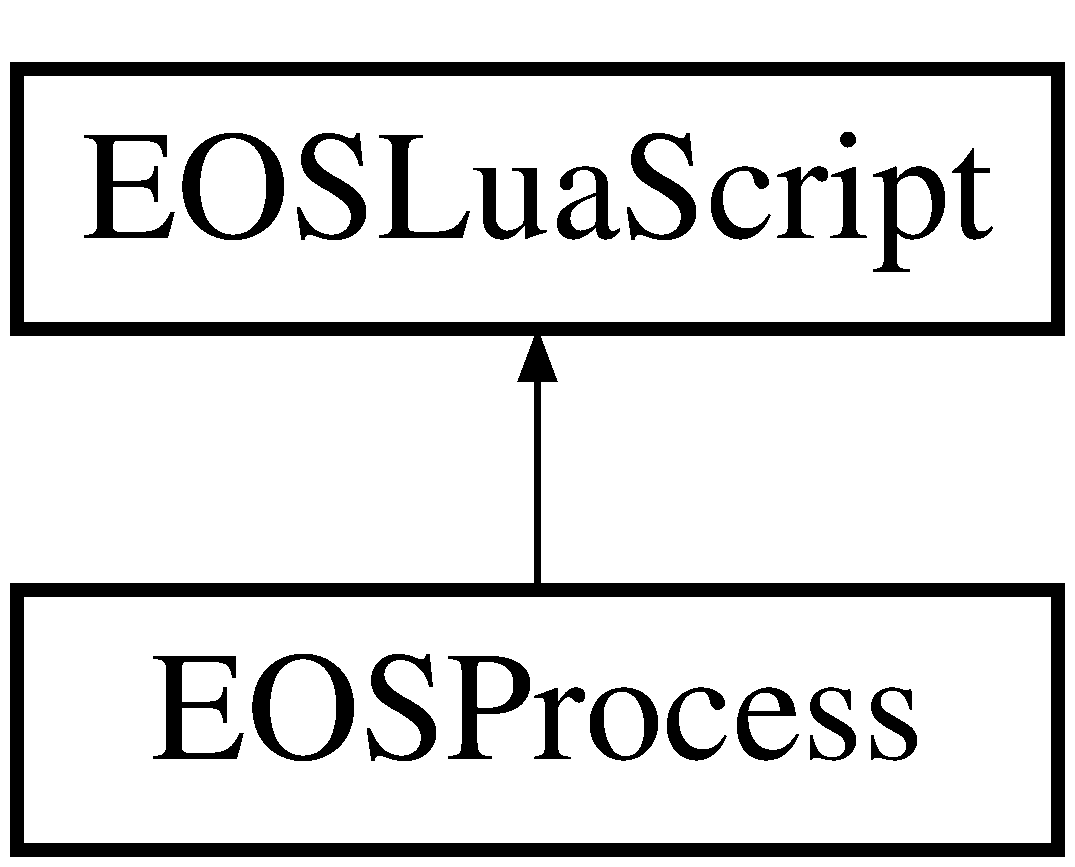
\includegraphics[height=2cm]{classEOSLuaScript}
\end{center}
\end{figure}
\subsection*{Public Member Functions}
\begin{CompactItemize}
\item 
\hyperlink{classEOSLuaScript_4983ae13c09b63b607885c0770655362}{EOSLuaScript} (\hyperlink{classEOSLuaEnvironment}{EOSLuaEnvironment} $\ast$luaEnvPtr, const char $\ast$scriptFileName)
\begin{CompactList}\small\item\em constructor \item\end{CompactList}\item 
virtual \hyperlink{classEOSLuaScript_0967a55fb7371b9e5808822ba184996b}{$\sim$EOSLuaScript} ()
\begin{CompactList}\small\item\em destructor \item\end{CompactList}\item 
bool \hyperlink{classEOSLuaScript_c1d576d2d3ffa64a9437a062f325a813}{compileBuffer} (unsigned char $\ast$bufferPtr, size\_\-t bufferSize)
\begin{CompactList}\small\item\em calls Lua compiler on Lua code stored in a memory buffer \item\end{CompactList}\item 
bool \hyperlink{classEOSLuaScript_7f00ff555be32da27000d51bc7ba420f}{selectScriptFunction} (const char $\ast$functionName)
\begin{CompactList}\small\item\em Selects a Lua Script function to call. \item\end{CompactList}\item 
void \hyperlink{classEOSLuaScript_a939a1d1daa1326a012e5e60e1b45f95}{addParam} (int intValue)
\begin{CompactList}\small\item\em loads integer parameter to the selected function \item\end{CompactList}\item 
void \hyperlink{classEOSLuaScript_1a6ac1c2783c000b1cf57b3a09c04cfc}{addParam} (float floatValue)
\begin{CompactList}\small\item\em loads floating point parameter to the selected function \item\end{CompactList}\item 
void \hyperlink{classEOSLuaScript_9a6e58cbb890391a8eb34cf22a0e7cfd}{addParam} (char $\ast$string)
\begin{CompactList}\small\item\em loads string parameter to the selected function \item\end{CompactList}\item 
bool \hyperlink{classEOSLuaScript_6d24519473b5a583d3ce89252a11e0ce}{go} (int nReturns=0)
\begin{CompactList}\small\item\em Runs the loaded script. \item\end{CompactList}\item 
bool \hyperlink{classEOSLuaScript_466d88c9afeec258536cd069b811f325}{scriptHasFunction} (const char $\ast$functionName)
\begin{CompactList}\small\item\em tests if the script contains a function with a given name \item\end{CompactList}\end{CompactItemize}
\subsection*{Protected Attributes}
\begin{CompactItemize}
\item 
\hyperlink{classEOSLuaEnvironment}{EOSLuaEnvironment} $\ast$ \hyperlink{classEOSLuaScript_4417b00b43ee03bc2120f76a3bb12d07}{luaEnv}
\begin{CompactList}\small\item\em pointer to the Lua runtime environment \item\end{CompactList}\item 
int \hyperlink{classEOSLuaScript_6ce277b904132a14459a929d6d8a5903}{luaThisRef}
\begin{CompactList}\small\item\em variable used to handle the \char`\"{}this\char`\"{} reference in scripts \item\end{CompactList}\item 
int \hyperlink{classEOSLuaScript_b86282ecf112d657fd92b29b4e21a40e}{numArgs}
\begin{CompactList}\small\item\em counts the number of parameters loaded in the stack for the lua function \item\end{CompactList}\item 
const char $\ast$ \hyperlink{classEOSLuaScript_f4fddb1fd2af7b266cb7b41f6b50a047}{currSelectedFuncName}
\begin{CompactList}\small\item\em contains the name of the current Lua function to call \item\end{CompactList}\item 
std::string \hyperlink{classEOSLuaScript_7ca6cc5f26c5cfad510e9391e5815d8c}{scriptName}
\begin{CompactList}\small\item\em contains the name of this script \item\end{CompactList}\end{CompactItemize}


\subsection{Detailed Description}
This class represents a single EOS Lua source script. 

\subsection{Constructor \& Destructor Documentation}
\hypertarget{classEOSLuaScript_4983ae13c09b63b607885c0770655362}{
\index{EOSLuaScript@{EOSLuaScript}!EOSLuaScript@{EOSLuaScript}}
\index{EOSLuaScript@{EOSLuaScript}!EOSLuaScript@{EOSLuaScript}}
\subsubsection[{EOSLuaScript}]{\setlength{\rightskip}{0pt plus 5cm}EOSLuaScript::EOSLuaScript ({\bf EOSLuaEnvironment} $\ast$ {\em luaEnvPtr}, \/  const char $\ast$ {\em scriptFileName})}}
\label{classEOSLuaScript_4983ae13c09b63b607885c0770655362}


constructor 

\hypertarget{classEOSLuaScript_0967a55fb7371b9e5808822ba184996b}{
\index{EOSLuaScript@{EOSLuaScript}!$\sim$EOSLuaScript@{$\sim$EOSLuaScript}}
\index{$\sim$EOSLuaScript@{$\sim$EOSLuaScript}!EOSLuaScript@{EOSLuaScript}}
\subsubsection[{$\sim$EOSLuaScript}]{\setlength{\rightskip}{0pt plus 5cm}EOSLuaScript::$\sim$EOSLuaScript ()\hspace{0.3cm}{\tt  \mbox{[}virtual\mbox{]}}}}
\label{classEOSLuaScript_0967a55fb7371b9e5808822ba184996b}


destructor 



\subsection{Member Function Documentation}
\hypertarget{classEOSLuaScript_c1d576d2d3ffa64a9437a062f325a813}{
\index{EOSLuaScript@{EOSLuaScript}!compileBuffer@{compileBuffer}}
\index{compileBuffer@{compileBuffer}!EOSLuaScript@{EOSLuaScript}}
\subsubsection[{compileBuffer}]{\setlength{\rightskip}{0pt plus 5cm}bool EOSLuaScript::compileBuffer (unsigned char $\ast$ {\em bufferPtr}, \/  size\_\-t {\em bufferSize})}}
\label{classEOSLuaScript_c1d576d2d3ffa64a9437a062f325a813}


calls Lua compiler on Lua code stored in a memory buffer 

\hypertarget{classEOSLuaScript_7f00ff555be32da27000d51bc7ba420f}{
\index{EOSLuaScript@{EOSLuaScript}!selectScriptFunction@{selectScriptFunction}}
\index{selectScriptFunction@{selectScriptFunction}!EOSLuaScript@{EOSLuaScript}}
\subsubsection[{selectScriptFunction}]{\setlength{\rightskip}{0pt plus 5cm}bool EOSLuaScript::selectScriptFunction (const char $\ast$ {\em functionName})}}
\label{classEOSLuaScript_7f00ff555be32da27000d51bc7ba420f}


Selects a Lua Script function to call. 

\hypertarget{classEOSLuaScript_a939a1d1daa1326a012e5e60e1b45f95}{
\index{EOSLuaScript@{EOSLuaScript}!addParam@{addParam}}
\index{addParam@{addParam}!EOSLuaScript@{EOSLuaScript}}
\subsubsection[{addParam}]{\setlength{\rightskip}{0pt plus 5cm}void EOSLuaScript::addParam (int {\em intValue})}}
\label{classEOSLuaScript_a939a1d1daa1326a012e5e60e1b45f95}


loads integer parameter to the selected function 

\hypertarget{classEOSLuaScript_1a6ac1c2783c000b1cf57b3a09c04cfc}{
\index{EOSLuaScript@{EOSLuaScript}!addParam@{addParam}}
\index{addParam@{addParam}!EOSLuaScript@{EOSLuaScript}}
\subsubsection[{addParam}]{\setlength{\rightskip}{0pt plus 5cm}void EOSLuaScript::addParam (float {\em floatValue})}}
\label{classEOSLuaScript_1a6ac1c2783c000b1cf57b3a09c04cfc}


loads floating point parameter to the selected function 

\hypertarget{classEOSLuaScript_9a6e58cbb890391a8eb34cf22a0e7cfd}{
\index{EOSLuaScript@{EOSLuaScript}!addParam@{addParam}}
\index{addParam@{addParam}!EOSLuaScript@{EOSLuaScript}}
\subsubsection[{addParam}]{\setlength{\rightskip}{0pt plus 5cm}void EOSLuaScript::addParam (char $\ast$ {\em string})}}
\label{classEOSLuaScript_9a6e58cbb890391a8eb34cf22a0e7cfd}


loads string parameter to the selected function 

\hypertarget{classEOSLuaScript_6d24519473b5a583d3ce89252a11e0ce}{
\index{EOSLuaScript@{EOSLuaScript}!go@{go}}
\index{go@{go}!EOSLuaScript@{EOSLuaScript}}
\subsubsection[{go}]{\setlength{\rightskip}{0pt plus 5cm}bool EOSLuaScript::go (int {\em nReturns} = {\tt 0})}}
\label{classEOSLuaScript_6d24519473b5a583d3ce89252a11e0ce}


Runs the loaded script. 

\hypertarget{classEOSLuaScript_466d88c9afeec258536cd069b811f325}{
\index{EOSLuaScript@{EOSLuaScript}!scriptHasFunction@{scriptHasFunction}}
\index{scriptHasFunction@{scriptHasFunction}!EOSLuaScript@{EOSLuaScript}}
\subsubsection[{scriptHasFunction}]{\setlength{\rightskip}{0pt plus 5cm}bool EOSLuaScript::scriptHasFunction (const char $\ast$ {\em functionName})}}
\label{classEOSLuaScript_466d88c9afeec258536cd069b811f325}


tests if the script contains a function with a given name 



\subsection{Field Documentation}
\hypertarget{classEOSLuaScript_4417b00b43ee03bc2120f76a3bb12d07}{
\index{EOSLuaScript@{EOSLuaScript}!luaEnv@{luaEnv}}
\index{luaEnv@{luaEnv}!EOSLuaScript@{EOSLuaScript}}
\subsubsection[{luaEnv}]{\setlength{\rightskip}{0pt plus 5cm}{\bf EOSLuaEnvironment}$\ast$ {\bf EOSLuaScript::luaEnv}\hspace{0.3cm}{\tt  \mbox{[}protected\mbox{]}}}}
\label{classEOSLuaScript_4417b00b43ee03bc2120f76a3bb12d07}


pointer to the Lua runtime environment 

\hypertarget{classEOSLuaScript_6ce277b904132a14459a929d6d8a5903}{
\index{EOSLuaScript@{EOSLuaScript}!luaThisRef@{luaThisRef}}
\index{luaThisRef@{luaThisRef}!EOSLuaScript@{EOSLuaScript}}
\subsubsection[{luaThisRef}]{\setlength{\rightskip}{0pt plus 5cm}int {\bf EOSLuaScript::luaThisRef}\hspace{0.3cm}{\tt  \mbox{[}protected\mbox{]}}}}
\label{classEOSLuaScript_6ce277b904132a14459a929d6d8a5903}


variable used to handle the \char`\"{}this\char`\"{} reference in scripts 

\hypertarget{classEOSLuaScript_b86282ecf112d657fd92b29b4e21a40e}{
\index{EOSLuaScript@{EOSLuaScript}!numArgs@{numArgs}}
\index{numArgs@{numArgs}!EOSLuaScript@{EOSLuaScript}}
\subsubsection[{numArgs}]{\setlength{\rightskip}{0pt plus 5cm}int {\bf EOSLuaScript::numArgs}\hspace{0.3cm}{\tt  \mbox{[}protected\mbox{]}}}}
\label{classEOSLuaScript_b86282ecf112d657fd92b29b4e21a40e}


counts the number of parameters loaded in the stack for the lua function 

\hypertarget{classEOSLuaScript_f4fddb1fd2af7b266cb7b41f6b50a047}{
\index{EOSLuaScript@{EOSLuaScript}!currSelectedFuncName@{currSelectedFuncName}}
\index{currSelectedFuncName@{currSelectedFuncName}!EOSLuaScript@{EOSLuaScript}}
\subsubsection[{currSelectedFuncName}]{\setlength{\rightskip}{0pt plus 5cm}const char$\ast$ {\bf EOSLuaScript::currSelectedFuncName}\hspace{0.3cm}{\tt  \mbox{[}protected\mbox{]}}}}
\label{classEOSLuaScript_f4fddb1fd2af7b266cb7b41f6b50a047}


contains the name of the current Lua function to call 

\hypertarget{classEOSLuaScript_7ca6cc5f26c5cfad510e9391e5815d8c}{
\index{EOSLuaScript@{EOSLuaScript}!scriptName@{scriptName}}
\index{scriptName@{scriptName}!EOSLuaScript@{EOSLuaScript}}
\subsubsection[{scriptName}]{\setlength{\rightskip}{0pt plus 5cm}std::string {\bf EOSLuaScript::scriptName}\hspace{0.3cm}{\tt  \mbox{[}protected\mbox{]}}}}
\label{classEOSLuaScript_7ca6cc5f26c5cfad510e9391e5815d8c}


contains the name of this script 



The documentation for this class was generated from the following files:\begin{CompactItemize}
\item 
\hyperlink{EOSLuaScript_8h}{EOSLuaScript.h}\item 
\hyperlink{EOSLuaScript_8cpp}{EOSLuaScript.cpp}\end{CompactItemize}

\hypertarget{classEOSLuaStackRestorer}{
\section{EOSLuaStackRestorer Class Reference}
\label{classEOSLuaStackRestorer}\index{EOSLuaStackRestorer@{EOSLuaStackRestorer}}
}
This class is used to keep Lua stack always in a consistent state {\em (based on code from Richard Shephard, published on CodeProject website: \href{http://www.codeproject.com/cpp/luaincpp.asp}{\tt http://www.codeproject.com/cpp/luaincpp.asp})\/}.  


{\tt \#include $<$EOSLuaStackRestorer.h$>$}

\subsection*{Public Member Functions}
\begin{CompactItemize}
\item 
\hyperlink{classEOSLuaStackRestorer_e3649dbb621699f8819b90a92cf99a9c}{EOSLuaStackRestorer} (\hyperlink{classEOSLuaEnvironment}{EOSLuaEnvironment} $\ast$luaEnv)
\item 
virtual \hyperlink{classEOSLuaStackRestorer_f884b6fb3dc476c864a541feec1a4450}{$\sim$EOSLuaStackRestorer} (void)
\end{CompactItemize}
\subsection*{Protected Attributes}
\begin{CompactItemize}
\item 
lua\_\-State $\ast$ \hyperlink{classEOSLuaStackRestorer_64d91d3f95091c585218086be99a2e9e}{luaState}
\item 
int \hyperlink{classEOSLuaStackRestorer_b974c1e60d9c0ec86e502457d6f6c1e5}{stackTop}
\end{CompactItemize}


\subsection{Detailed Description}
This class is used to keep Lua stack always in a consistent state {\em (based on code from Richard Shephard, published on CodeProject website: \href{http://www.codeproject.com/cpp/luaincpp.asp}{\tt http://www.codeproject.com/cpp/luaincpp.asp})\/}. 

\subsection{Constructor \& Destructor Documentation}
\hypertarget{classEOSLuaStackRestorer_e3649dbb621699f8819b90a92cf99a9c}{
\index{EOSLuaStackRestorer@{EOSLuaStackRestorer}!EOSLuaStackRestorer@{EOSLuaStackRestorer}}
\index{EOSLuaStackRestorer@{EOSLuaStackRestorer}!EOSLuaStackRestorer@{EOSLuaStackRestorer}}
\subsubsection[{EOSLuaStackRestorer}]{\setlength{\rightskip}{0pt plus 5cm}EOSLuaStackRestorer::EOSLuaStackRestorer ({\bf EOSLuaEnvironment} $\ast$ {\em luaEnv})\hspace{0.3cm}{\tt  \mbox{[}inline\mbox{]}}}}
\label{classEOSLuaStackRestorer_e3649dbb621699f8819b90a92cf99a9c}


\hypertarget{classEOSLuaStackRestorer_f884b6fb3dc476c864a541feec1a4450}{
\index{EOSLuaStackRestorer@{EOSLuaStackRestorer}!$\sim$EOSLuaStackRestorer@{$\sim$EOSLuaStackRestorer}}
\index{$\sim$EOSLuaStackRestorer@{$\sim$EOSLuaStackRestorer}!EOSLuaStackRestorer@{EOSLuaStackRestorer}}
\subsubsection[{$\sim$EOSLuaStackRestorer}]{\setlength{\rightskip}{0pt plus 5cm}virtual EOSLuaStackRestorer::$\sim$EOSLuaStackRestorer (void)\hspace{0.3cm}{\tt  \mbox{[}inline, virtual\mbox{]}}}}
\label{classEOSLuaStackRestorer_f884b6fb3dc476c864a541feec1a4450}




\subsection{Field Documentation}
\hypertarget{classEOSLuaStackRestorer_64d91d3f95091c585218086be99a2e9e}{
\index{EOSLuaStackRestorer@{EOSLuaStackRestorer}!luaState@{luaState}}
\index{luaState@{luaState}!EOSLuaStackRestorer@{EOSLuaStackRestorer}}
\subsubsection[{luaState}]{\setlength{\rightskip}{0pt plus 5cm}lua\_\-State$\ast$ {\bf EOSLuaStackRestorer::luaState}\hspace{0.3cm}{\tt  \mbox{[}protected\mbox{]}}}}
\label{classEOSLuaStackRestorer_64d91d3f95091c585218086be99a2e9e}


\hypertarget{classEOSLuaStackRestorer_b974c1e60d9c0ec86e502457d6f6c1e5}{
\index{EOSLuaStackRestorer@{EOSLuaStackRestorer}!stackTop@{stackTop}}
\index{stackTop@{stackTop}!EOSLuaStackRestorer@{EOSLuaStackRestorer}}
\subsubsection[{stackTop}]{\setlength{\rightskip}{0pt plus 5cm}int {\bf EOSLuaStackRestorer::stackTop}\hspace{0.3cm}{\tt  \mbox{[}protected\mbox{]}}}}
\label{classEOSLuaStackRestorer_b974c1e60d9c0ec86e502457d6f6c1e5}




The documentation for this class was generated from the following file:\begin{CompactItemize}
\item 
\hyperlink{EOSLuaStackRestorer_8h}{EOSLuaStackRestorer.h}\end{CompactItemize}

\hypertarget{classEOSLuaThisRestorer}{
\section{EOSLuaThisRestorer Class Reference}
\label{classEOSLuaThisRestorer}\index{EOSLuaThisRestorer@{EOSLuaThisRestorer}}
}
This class is used to load the correct \char`\"{}this\char`\"{} reference each time the execution enters on a new script {\em (based on code from Richard Shephard, published on CodeProject website: \href{http://www.codeproject.com/cpp/luaincpp.asp}{\tt http://www.codeproject.com/cpp/luaincpp.asp})\/}.  


{\tt \#include $<$EOSLuaThisRestorer.h$>$}

\subsection*{Public Member Functions}
\begin{CompactItemize}
\item 
\hyperlink{classEOSLuaThisRestorer_81ca0a43271615529a47f3983c5ffe30}{EOSLuaThisRestorer} (\hyperlink{classEOSLuaEnvironment}{EOSLuaEnvironment} $\ast$\hyperlink{classEOSLuaThisRestorer_97a1c3bec2094802ad9976b63ec6269f}{luaEnv}, int thisRef)
\item 
virtual \hyperlink{classEOSLuaThisRestorer_f674e78a80a788f6ceaaf3762572ab9d}{$\sim$EOSLuaThisRestorer} ()
\end{CompactItemize}
\subsection*{Protected Attributes}
\begin{CompactItemize}
\item 
int \hyperlink{classEOSLuaThisRestorer_ab1eec278bb8cda42e152ec7d82c8d3a}{oldThisRef}
\item 
\hyperlink{classEOSLuaEnvironment}{EOSLuaEnvironment} $\ast$ \hyperlink{classEOSLuaThisRestorer_97a1c3bec2094802ad9976b63ec6269f}{luaEnv}
\end{CompactItemize}


\subsection{Detailed Description}
This class is used to load the correct \char`\"{}this\char`\"{} reference each time the execution enters on a new script {\em (based on code from Richard Shephard, published on CodeProject website: \href{http://www.codeproject.com/cpp/luaincpp.asp}{\tt http://www.codeproject.com/cpp/luaincpp.asp})\/}. 

\subsection{Constructor \& Destructor Documentation}
\hypertarget{classEOSLuaThisRestorer_81ca0a43271615529a47f3983c5ffe30}{
\index{EOSLuaThisRestorer@{EOSLuaThisRestorer}!EOSLuaThisRestorer@{EOSLuaThisRestorer}}
\index{EOSLuaThisRestorer@{EOSLuaThisRestorer}!EOSLuaThisRestorer@{EOSLuaThisRestorer}}
\subsubsection[{EOSLuaThisRestorer}]{\setlength{\rightskip}{0pt plus 5cm}EOSLuaThisRestorer::EOSLuaThisRestorer ({\bf EOSLuaEnvironment} $\ast$ {\em luaEnv}, \/  int {\em thisRef})\hspace{0.3cm}{\tt  \mbox{[}inline\mbox{]}}}}
\label{classEOSLuaThisRestorer_81ca0a43271615529a47f3983c5ffe30}


\hypertarget{classEOSLuaThisRestorer_f674e78a80a788f6ceaaf3762572ab9d}{
\index{EOSLuaThisRestorer@{EOSLuaThisRestorer}!$\sim$EOSLuaThisRestorer@{$\sim$EOSLuaThisRestorer}}
\index{$\sim$EOSLuaThisRestorer@{$\sim$EOSLuaThisRestorer}!EOSLuaThisRestorer@{EOSLuaThisRestorer}}
\subsubsection[{$\sim$EOSLuaThisRestorer}]{\setlength{\rightskip}{0pt plus 5cm}virtual EOSLuaThisRestorer::$\sim$EOSLuaThisRestorer ()\hspace{0.3cm}{\tt  \mbox{[}inline, virtual\mbox{]}}}}
\label{classEOSLuaThisRestorer_f674e78a80a788f6ceaaf3762572ab9d}




\subsection{Field Documentation}
\hypertarget{classEOSLuaThisRestorer_ab1eec278bb8cda42e152ec7d82c8d3a}{
\index{EOSLuaThisRestorer@{EOSLuaThisRestorer}!oldThisRef@{oldThisRef}}
\index{oldThisRef@{oldThisRef}!EOSLuaThisRestorer@{EOSLuaThisRestorer}}
\subsubsection[{oldThisRef}]{\setlength{\rightskip}{0pt plus 5cm}int {\bf EOSLuaThisRestorer::oldThisRef}\hspace{0.3cm}{\tt  \mbox{[}protected\mbox{]}}}}
\label{classEOSLuaThisRestorer_ab1eec278bb8cda42e152ec7d82c8d3a}


\hypertarget{classEOSLuaThisRestorer_97a1c3bec2094802ad9976b63ec6269f}{
\index{EOSLuaThisRestorer@{EOSLuaThisRestorer}!luaEnv@{luaEnv}}
\index{luaEnv@{luaEnv}!EOSLuaThisRestorer@{EOSLuaThisRestorer}}
\subsubsection[{luaEnv}]{\setlength{\rightskip}{0pt plus 5cm}{\bf EOSLuaEnvironment}$\ast$ {\bf EOSLuaThisRestorer::luaEnv}\hspace{0.3cm}{\tt  \mbox{[}protected\mbox{]}}}}
\label{classEOSLuaThisRestorer_97a1c3bec2094802ad9976b63ec6269f}




The documentation for this class was generated from the following file:\begin{CompactItemize}
\item 
\hyperlink{EOSLuaThisRestorer_8h}{EOSLuaThisRestorer.h}\end{CompactItemize}

\hypertarget{classEOSMessage}{
\section{EOSMessage Class Reference}
\label{classEOSMessage}\index{EOSMessage@{EOSMessage}}
}
This class models the EOS Message Structure.  


{\tt \#include $<$EOSMessage.h$>$}

\subsection*{Public Member Functions}
\begin{CompactItemize}
\item 
\hyperlink{classEOSMessage_4f107c4d2bc222fff75d0a600f8ebfa9}{EOSMessage} (const char $\ast$messageClass)
\begin{CompactList}\small\item\em constructor \item\end{CompactList}\item 
\hyperlink{classEOSMessage_57e0677a37c99625d6480d91a910a8bc}{$\sim$EOSMessage} ()
\begin{CompactList}\small\item\em destructor \item\end{CompactList}\item 
void \hyperlink{classEOSMessage_7eea6ddaa2fc88e278f1b8916a72da94}{addValue} (const char $\ast$valueKey, bool valueData)
\begin{CompactList}\small\item\em pushes a boolean value field in the message structure \item\end{CompactList}\item 
void \hyperlink{classEOSMessage_fa321169de1d36442816d52085a2d7c8}{addValue} (const char $\ast$valueKey, double valueData)
\begin{CompactList}\small\item\em pushes a numeric value field in the message structure \item\end{CompactList}\item 
void \hyperlink{classEOSMessage_4e26aa7bc47fb80d6b06cbdb12b63a51}{addValue} (const char $\ast$valueKey, const char $\ast$valueData)
\begin{CompactList}\small\item\em pushes a string value field in the message structure \item\end{CompactList}\item 
void \hyperlink{classEOSMessage_2acc24a0b1bd887a34357057a0678537}{toLuaMessageBoardTable} (lua\_\-State $\ast$luaRuntime)
\begin{CompactList}\small\item\em loads all message fields in the Lua runtime \hyperlink{classEOSMessage}{EOSMessage} global table \item\end{CompactList}\item 
void \hyperlink{classEOSMessage_fee56421daea7a52d9c9bfccb95e92ee}{setSender} (const char $\ast$sender)
\begin{CompactList}\small\item\em sets sender process name \item\end{CompactList}\item 
void \hyperlink{classEOSMessage_cd7733e73deb926208b222b7f7c50d4d}{setReceiver} (const char $\ast$receiver)
\begin{CompactList}\small\item\em sets receiver process name \item\end{CompactList}\item 
std::string \& \hyperlink{classEOSMessage_1d5409e96cc5af7426f36b4e7e90e745}{getSender} ()
\begin{CompactList}\small\item\em returns sender process name \item\end{CompactList}\item 
std::string \& \hyperlink{classEOSMessage_190437e488f9966c3a66efc6343dd2ff}{getReceiver} ()
\begin{CompactList}\small\item\em returns receiver process name \item\end{CompactList}\end{CompactItemize}
\subsection*{Private Attributes}
\begin{CompactItemize}
\item 
std::vector$<$ \hyperlink{classMessageField}{MessageField} $\ast$ $>$ \hyperlink{classEOSMessage_96ec4e4136d8098a9de40eda92f49dc2}{values}
\begin{CompactList}\small\item\em message fields vector \item\end{CompactList}\item 
std::string \hyperlink{classEOSMessage_0d4527e99c9d665cd65b3cd753ef59df}{senderName}
\begin{CompactList}\small\item\em this string holds sender name \item\end{CompactList}\item 
std::string \hyperlink{classEOSMessage_e2b133e9168915c7c0daf1116aed816b}{receiverName}
\begin{CompactList}\small\item\em this string holds receiver name \item\end{CompactList}\end{CompactItemize}


\subsection{Detailed Description}
This class models the EOS Message Structure. 

\subsection{Constructor \& Destructor Documentation}
\hypertarget{classEOSMessage_4f107c4d2bc222fff75d0a600f8ebfa9}{
\index{EOSMessage@{EOSMessage}!EOSMessage@{EOSMessage}}
\index{EOSMessage@{EOSMessage}!EOSMessage@{EOSMessage}}
\subsubsection[{EOSMessage}]{\setlength{\rightskip}{0pt plus 5cm}EOSMessage::EOSMessage (const char $\ast$ {\em messageClass})}}
\label{classEOSMessage_4f107c4d2bc222fff75d0a600f8ebfa9}


constructor 

\hypertarget{classEOSMessage_57e0677a37c99625d6480d91a910a8bc}{
\index{EOSMessage@{EOSMessage}!$\sim$EOSMessage@{$\sim$EOSMessage}}
\index{$\sim$EOSMessage@{$\sim$EOSMessage}!EOSMessage@{EOSMessage}}
\subsubsection[{$\sim$EOSMessage}]{\setlength{\rightskip}{0pt plus 5cm}EOSMessage::$\sim$EOSMessage ()}}
\label{classEOSMessage_57e0677a37c99625d6480d91a910a8bc}


destructor 



\subsection{Member Function Documentation}
\hypertarget{classEOSMessage_7eea6ddaa2fc88e278f1b8916a72da94}{
\index{EOSMessage@{EOSMessage}!addValue@{addValue}}
\index{addValue@{addValue}!EOSMessage@{EOSMessage}}
\subsubsection[{addValue}]{\setlength{\rightskip}{0pt plus 5cm}void EOSMessage::addValue (const char $\ast$ {\em valueKey}, \/  bool {\em valueData})}}
\label{classEOSMessage_7eea6ddaa2fc88e278f1b8916a72da94}


pushes a boolean value field in the message structure 

\hypertarget{classEOSMessage_fa321169de1d36442816d52085a2d7c8}{
\index{EOSMessage@{EOSMessage}!addValue@{addValue}}
\index{addValue@{addValue}!EOSMessage@{EOSMessage}}
\subsubsection[{addValue}]{\setlength{\rightskip}{0pt plus 5cm}void EOSMessage::addValue (const char $\ast$ {\em valueKey}, \/  double {\em valueData})}}
\label{classEOSMessage_fa321169de1d36442816d52085a2d7c8}


pushes a numeric value field in the message structure 

\hypertarget{classEOSMessage_4e26aa7bc47fb80d6b06cbdb12b63a51}{
\index{EOSMessage@{EOSMessage}!addValue@{addValue}}
\index{addValue@{addValue}!EOSMessage@{EOSMessage}}
\subsubsection[{addValue}]{\setlength{\rightskip}{0pt plus 5cm}void EOSMessage::addValue (const char $\ast$ {\em valueKey}, \/  const char $\ast$ {\em valueData})}}
\label{classEOSMessage_4e26aa7bc47fb80d6b06cbdb12b63a51}


pushes a string value field in the message structure 

\hypertarget{classEOSMessage_2acc24a0b1bd887a34357057a0678537}{
\index{EOSMessage@{EOSMessage}!toLuaMessageBoardTable@{toLuaMessageBoardTable}}
\index{toLuaMessageBoardTable@{toLuaMessageBoardTable}!EOSMessage@{EOSMessage}}
\subsubsection[{toLuaMessageBoardTable}]{\setlength{\rightskip}{0pt plus 5cm}void EOSMessage::toLuaMessageBoardTable (lua\_\-State $\ast$ {\em luaRuntime})}}
\label{classEOSMessage_2acc24a0b1bd887a34357057a0678537}


loads all message fields in the Lua runtime \hyperlink{classEOSMessage}{EOSMessage} global table 

\hypertarget{classEOSMessage_fee56421daea7a52d9c9bfccb95e92ee}{
\index{EOSMessage@{EOSMessage}!setSender@{setSender}}
\index{setSender@{setSender}!EOSMessage@{EOSMessage}}
\subsubsection[{setSender}]{\setlength{\rightskip}{0pt plus 5cm}void EOSMessage::setSender (const char $\ast$ {\em sender})\hspace{0.3cm}{\tt  \mbox{[}inline\mbox{]}}}}
\label{classEOSMessage_fee56421daea7a52d9c9bfccb95e92ee}


sets sender process name 

\hypertarget{classEOSMessage_cd7733e73deb926208b222b7f7c50d4d}{
\index{EOSMessage@{EOSMessage}!setReceiver@{setReceiver}}
\index{setReceiver@{setReceiver}!EOSMessage@{EOSMessage}}
\subsubsection[{setReceiver}]{\setlength{\rightskip}{0pt plus 5cm}void EOSMessage::setReceiver (const char $\ast$ {\em receiver})\hspace{0.3cm}{\tt  \mbox{[}inline\mbox{]}}}}
\label{classEOSMessage_cd7733e73deb926208b222b7f7c50d4d}


sets receiver process name 

\hypertarget{classEOSMessage_1d5409e96cc5af7426f36b4e7e90e745}{
\index{EOSMessage@{EOSMessage}!getSender@{getSender}}
\index{getSender@{getSender}!EOSMessage@{EOSMessage}}
\subsubsection[{getSender}]{\setlength{\rightskip}{0pt plus 5cm}std::string\& EOSMessage::getSender ()\hspace{0.3cm}{\tt  \mbox{[}inline\mbox{]}}}}
\label{classEOSMessage_1d5409e96cc5af7426f36b4e7e90e745}


returns sender process name 

\hypertarget{classEOSMessage_190437e488f9966c3a66efc6343dd2ff}{
\index{EOSMessage@{EOSMessage}!getReceiver@{getReceiver}}
\index{getReceiver@{getReceiver}!EOSMessage@{EOSMessage}}
\subsubsection[{getReceiver}]{\setlength{\rightskip}{0pt plus 5cm}std::string\& EOSMessage::getReceiver ()\hspace{0.3cm}{\tt  \mbox{[}inline\mbox{]}}}}
\label{classEOSMessage_190437e488f9966c3a66efc6343dd2ff}


returns receiver process name 



\subsection{Field Documentation}
\hypertarget{classEOSMessage_96ec4e4136d8098a9de40eda92f49dc2}{
\index{EOSMessage@{EOSMessage}!values@{values}}
\index{values@{values}!EOSMessage@{EOSMessage}}
\subsubsection[{values}]{\setlength{\rightskip}{0pt plus 5cm}std::vector$<${\bf MessageField}$\ast$$>$ {\bf EOSMessage::values}\hspace{0.3cm}{\tt  \mbox{[}private\mbox{]}}}}
\label{classEOSMessage_96ec4e4136d8098a9de40eda92f49dc2}


message fields vector 

\hypertarget{classEOSMessage_0d4527e99c9d665cd65b3cd753ef59df}{
\index{EOSMessage@{EOSMessage}!senderName@{senderName}}
\index{senderName@{senderName}!EOSMessage@{EOSMessage}}
\subsubsection[{senderName}]{\setlength{\rightskip}{0pt plus 5cm}std::string {\bf EOSMessage::senderName}\hspace{0.3cm}{\tt  \mbox{[}private\mbox{]}}}}
\label{classEOSMessage_0d4527e99c9d665cd65b3cd753ef59df}


this string holds sender name 

\hypertarget{classEOSMessage_e2b133e9168915c7c0daf1116aed816b}{
\index{EOSMessage@{EOSMessage}!receiverName@{receiverName}}
\index{receiverName@{receiverName}!EOSMessage@{EOSMessage}}
\subsubsection[{receiverName}]{\setlength{\rightskip}{0pt plus 5cm}std::string {\bf EOSMessage::receiverName}\hspace{0.3cm}{\tt  \mbox{[}private\mbox{]}}}}
\label{classEOSMessage_e2b133e9168915c7c0daf1116aed816b}


this string holds receiver name 



The documentation for this class was generated from the following files:\begin{CompactItemize}
\item 
\hyperlink{EOSMessage_8h}{EOSMessage.h}\item 
\hyperlink{EOSMessage_8cpp}{EOSMessage.cpp}\end{CompactItemize}

\hypertarget{classEOSProcess}{
\section{EOSProcess Class Reference}
\label{classEOSProcess}\index{EOSProcess@{EOSProcess}}
}
Class used to model an EOS Process (a single script instance).  


{\tt \#include $<$EOSProcess.h$>$}

Inheritance diagram for EOSProcess::\begin{figure}[H]
\begin{center}
\leavevmode
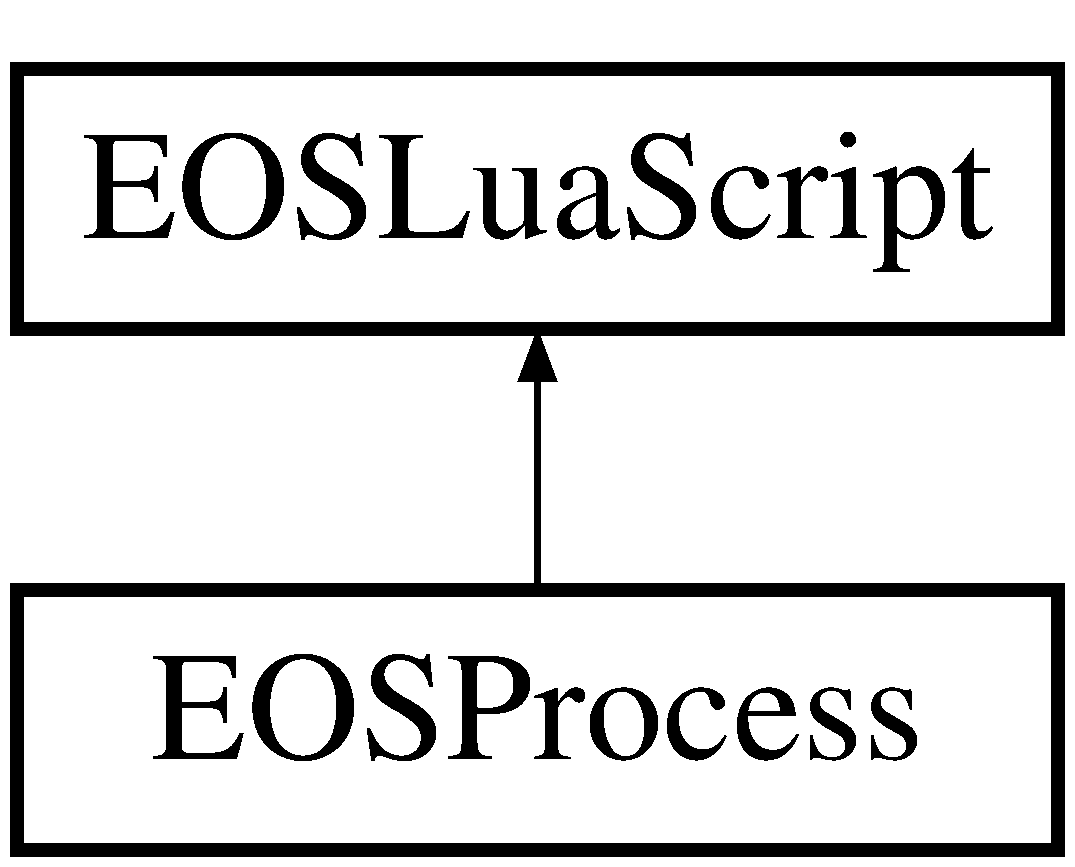
\includegraphics[height=2cm]{classEOSProcess}
\end{center}
\end{figure}
\subsection*{Public Member Functions}
\begin{CompactItemize}
\item 
\hyperlink{classEOSProcess_7c1ceeba22b5a334c0f95e32facddbea}{EOSProcess} (\hyperlink{classEOSLuaEnvironment}{EOSLuaEnvironment} $\ast$luaEnvPtr, \hyperlink{classEOSScriptManager}{EOSScriptManager} $\ast$scriptManagerPtr, const char $\ast$processName, const char $\ast$\hyperlink{classEOSLuaScript_7ca6cc5f26c5cfad510e9391e5815d8c}{scriptName})
\begin{CompactList}\small\item\em constructor \item\end{CompactList}\item 
\hyperlink{classEOSProcess_4204e2edd0f82d46409d37cbf309c8c6}{$\sim$EOSProcess} ()
\begin{CompactList}\small\item\em destructor \item\end{CompactList}\item 
bool \hyperlink{classEOSProcess_e595b8a353aac17d1ded7811d137a0ca}{init} ()
\begin{CompactList}\small\item\em executes \char`\"{}init\char`\"{} function from script \item\end{CompactList}\item 
bool \hyperlink{classEOSProcess_c141df99c0216969bc8b6b463f12b924}{update} ()
\begin{CompactList}\small\item\em executes \char`\"{}update\char`\"{} function from script \item\end{CompactList}\item 
bool \hyperlink{classEOSProcess_224e00ab735c33b4c5a4e58b9fe1826c}{cleanup} ()
\begin{CompactList}\small\item\em executes \char`\"{}cleanup\char`\"{} function from script \item\end{CompactList}\item 
void \hyperlink{classEOSProcess_bdaf60e60530702981c1d4ac5ceb4c3e}{processMessage} (\hyperlink{classEOSMessage}{EOSMessage} $\ast$message)
\begin{CompactList}\small\item\em executes \char`\"{}processMessage\char`\"{} function from script \item\end{CompactList}\item 
bool \hyperlink{classEOSProcess_e0e33032bb4be23f342515af1a3ff911}{isActive} ()
\begin{CompactList}\small\item\em returns the current activity status of this process \item\end{CompactList}\item 
bool \hyperlink{classEOSProcess_b5760c226c46227d395ec2e8fef7d340}{setActive} (bool status)
\begin{CompactList}\small\item\em sets the current activity status of this process \item\end{CompactList}\item 
bool \hyperlink{classEOSProcess_d5f8f932b1194afba3e3e4f37883e29a}{isGarbaged} ()
\begin{CompactList}\small\item\em returns the current garbage status of this process \item\end{CompactList}\item 
void \hyperlink{classEOSProcess_bec41530a483ecc6b9b35b34388515ec}{garbage} ()
\begin{CompactList}\small\item\em puts this process in \char`\"{}garbaged\char`\"{} status (a way to kill and deallocate it) \item\end{CompactList}\item 
bool \hyperlink{classEOSLuaScript_c1d576d2d3ffa64a9437a062f325a813}{compileBuffer} (unsigned char $\ast$bufferPtr, size\_\-t bufferSize)
\begin{CompactList}\small\item\em calls Lua compiler on Lua code stored in a memory buffer \item\end{CompactList}\item 
bool \hyperlink{classEOSLuaScript_7f00ff555be32da27000d51bc7ba420f}{selectScriptFunction} (const char $\ast$functionName)
\begin{CompactList}\small\item\em Selects a Lua Script function to call. \item\end{CompactList}\item 
void \hyperlink{classEOSLuaScript_a939a1d1daa1326a012e5e60e1b45f95}{addParam} (int intValue)
\begin{CompactList}\small\item\em loads integer parameter to the selected function \item\end{CompactList}\item 
void \hyperlink{classEOSLuaScript_1a6ac1c2783c000b1cf57b3a09c04cfc}{addParam} (float floatValue)
\begin{CompactList}\small\item\em loads floating point parameter to the selected function \item\end{CompactList}\item 
void \hyperlink{classEOSLuaScript_9a6e58cbb890391a8eb34cf22a0e7cfd}{addParam} (char $\ast$string)
\begin{CompactList}\small\item\em loads string parameter to the selected function \item\end{CompactList}\item 
bool \hyperlink{classEOSLuaScript_6d24519473b5a583d3ce89252a11e0ce}{go} (int nReturns=0)
\begin{CompactList}\small\item\em Runs the loaded script. \item\end{CompactList}\item 
bool \hyperlink{classEOSLuaScript_466d88c9afeec258536cd069b811f325}{scriptHasFunction} (const char $\ast$functionName)
\begin{CompactList}\small\item\em tests if the script contains a function with a given name \item\end{CompactList}\end{CompactItemize}
\subsection*{Protected Attributes}
\begin{CompactItemize}
\item 
\hyperlink{classEOSLuaEnvironment}{EOSLuaEnvironment} $\ast$ \hyperlink{classEOSLuaScript_4417b00b43ee03bc2120f76a3bb12d07}{luaEnv}
\begin{CompactList}\small\item\em pointer to the Lua runtime environment \item\end{CompactList}\item 
int \hyperlink{classEOSLuaScript_6ce277b904132a14459a929d6d8a5903}{luaThisRef}
\begin{CompactList}\small\item\em variable used to handle the \char`\"{}this\char`\"{} reference in scripts \item\end{CompactList}\item 
int \hyperlink{classEOSLuaScript_b86282ecf112d657fd92b29b4e21a40e}{numArgs}
\begin{CompactList}\small\item\em counts the number of parameters loaded in the stack for the lua function \item\end{CompactList}\item 
const char $\ast$ \hyperlink{classEOSLuaScript_f4fddb1fd2af7b266cb7b41f6b50a047}{currSelectedFuncName}
\begin{CompactList}\small\item\em contains the name of the current Lua function to call \item\end{CompactList}\item 
std::string \hyperlink{classEOSLuaScript_7ca6cc5f26c5cfad510e9391e5815d8c}{scriptName}
\begin{CompactList}\small\item\em contains the name of this script \item\end{CompactList}\end{CompactItemize}
\subsection*{Private Member Functions}
\begin{CompactItemize}
\item 
void \hyperlink{classEOSProcess_f05d10a4411470314d51dea89c980967}{pushProcessName} ()
\begin{CompactList}\small\item\em puts this process name in the Lua environment, under \char`\"{}this.processName\char`\"{} \item\end{CompactList}\item 
void \hyperlink{classEOSProcess_9beab4f3d93c870ce78905dff204ed14}{clearProcessName} ()
\begin{CompactList}\small\item\em clears \char`\"{}this.processName\char`\"{} variable in the Lua environment \item\end{CompactList}\end{CompactItemize}
\subsection*{Private Attributes}
\begin{CompactItemize}
\item 
char \hyperlink{classEOSProcess_318b6a6c7ab85ac4b9ecad280cd3fe5d}{luaChunk} \mbox{[}MAXCHUNKLENGTH+1\mbox{]}
\begin{CompactList}\small\item\em holds a temporary lua source buffer \item\end{CompactList}\item 
const char $\ast$ \hyperlink{classEOSProcess_19fe017cf86629e8783b745e5f88a5a7}{thisProcessName}
\begin{CompactList}\small\item\em holds the name of this process \item\end{CompactList}\item 
bool \hyperlink{classEOSProcess_223622c13ea24b06079078ac0910925f}{active}
\begin{CompactList}\small\item\em holds the current activity status of this process \item\end{CompactList}\item 
bool \hyperlink{classEOSProcess_69b4f5d326f9fbbda1ddad22b42f80b9}{valid}
\begin{CompactList}\small\item\em used to trace internally the validity of this process \item\end{CompactList}\item 
bool \hyperlink{classEOSProcess_97ff1c226411207b2fe0582b1b67603b}{initialized}
\begin{CompactList}\small\item\em used to trace internally the initialization status of this process \item\end{CompactList}\item 
bool \hyperlink{classEOSProcess_a3bc6045894d86d9d64d9ad8ab610684}{garbaged}
\begin{CompactList}\small\item\em holds the current \char`\"{}garbage\char`\"{} status of this process \item\end{CompactList}\item 
\hyperlink{classEOSScriptManager}{EOSScriptManager} $\ast$ \hyperlink{classEOSProcess_86d146cc56d2a9aa68fdb6ab3ded52f0}{scriptManager}
\begin{CompactList}\small\item\em pointer to the ScriptManager class \item\end{CompactList}\end{CompactItemize}


\subsection{Detailed Description}
Class used to model an EOS Process (a single script instance). 

Many processes can share the same script source. 

\subsection{Constructor \& Destructor Documentation}
\hypertarget{classEOSProcess_7c1ceeba22b5a334c0f95e32facddbea}{
\index{EOSProcess@{EOSProcess}!EOSProcess@{EOSProcess}}
\index{EOSProcess@{EOSProcess}!EOSProcess@{EOSProcess}}
\subsubsection[{EOSProcess}]{\setlength{\rightskip}{0pt plus 5cm}EOSProcess::EOSProcess ({\bf EOSLuaEnvironment} $\ast$ {\em luaEnvPtr}, \/  {\bf EOSScriptManager} $\ast$ {\em scriptManagerPtr}, \/  const char $\ast$ {\em processName}, \/  const char $\ast$ {\em scriptName})\hspace{0.3cm}{\tt  \mbox{[}inline\mbox{]}}}}
\label{classEOSProcess_7c1ceeba22b5a334c0f95e32facddbea}


constructor 

\hypertarget{classEOSProcess_4204e2edd0f82d46409d37cbf309c8c6}{
\index{EOSProcess@{EOSProcess}!$\sim$EOSProcess@{$\sim$EOSProcess}}
\index{$\sim$EOSProcess@{$\sim$EOSProcess}!EOSProcess@{EOSProcess}}
\subsubsection[{$\sim$EOSProcess}]{\setlength{\rightskip}{0pt plus 5cm}EOSProcess::$\sim$EOSProcess ()\hspace{0.3cm}{\tt  \mbox{[}inline\mbox{]}}}}
\label{classEOSProcess_4204e2edd0f82d46409d37cbf309c8c6}


destructor 



\subsection{Member Function Documentation}
\hypertarget{classEOSProcess_e595b8a353aac17d1ded7811d137a0ca}{
\index{EOSProcess@{EOSProcess}!init@{init}}
\index{init@{init}!EOSProcess@{EOSProcess}}
\subsubsection[{init}]{\setlength{\rightskip}{0pt plus 5cm}bool EOSProcess::init ()\hspace{0.3cm}{\tt  \mbox{[}inline\mbox{]}}}}
\label{classEOSProcess_e595b8a353aac17d1ded7811d137a0ca}


executes \char`\"{}init\char`\"{} function from script 

\hypertarget{classEOSProcess_c141df99c0216969bc8b6b463f12b924}{
\index{EOSProcess@{EOSProcess}!update@{update}}
\index{update@{update}!EOSProcess@{EOSProcess}}
\subsubsection[{update}]{\setlength{\rightskip}{0pt plus 5cm}bool EOSProcess::update ()\hspace{0.3cm}{\tt  \mbox{[}inline\mbox{]}}}}
\label{classEOSProcess_c141df99c0216969bc8b6b463f12b924}


executes \char`\"{}update\char`\"{} function from script 

\hypertarget{classEOSProcess_224e00ab735c33b4c5a4e58b9fe1826c}{
\index{EOSProcess@{EOSProcess}!cleanup@{cleanup}}
\index{cleanup@{cleanup}!EOSProcess@{EOSProcess}}
\subsubsection[{cleanup}]{\setlength{\rightskip}{0pt plus 5cm}bool EOSProcess::cleanup ()\hspace{0.3cm}{\tt  \mbox{[}inline\mbox{]}}}}
\label{classEOSProcess_224e00ab735c33b4c5a4e58b9fe1826c}


executes \char`\"{}cleanup\char`\"{} function from script 

\hypertarget{classEOSProcess_bdaf60e60530702981c1d4ac5ceb4c3e}{
\index{EOSProcess@{EOSProcess}!processMessage@{processMessage}}
\index{processMessage@{processMessage}!EOSProcess@{EOSProcess}}
\subsubsection[{processMessage}]{\setlength{\rightskip}{0pt plus 5cm}void EOSProcess::processMessage ({\bf EOSMessage} $\ast$ {\em message})}}
\label{classEOSProcess_bdaf60e60530702981c1d4ac5ceb4c3e}


executes \char`\"{}processMessage\char`\"{} function from script 

\hypertarget{classEOSProcess_e0e33032bb4be23f342515af1a3ff911}{
\index{EOSProcess@{EOSProcess}!isActive@{isActive}}
\index{isActive@{isActive}!EOSProcess@{EOSProcess}}
\subsubsection[{isActive}]{\setlength{\rightskip}{0pt plus 5cm}bool EOSProcess::isActive ()\hspace{0.3cm}{\tt  \mbox{[}inline\mbox{]}}}}
\label{classEOSProcess_e0e33032bb4be23f342515af1a3ff911}


returns the current activity status of this process 

\hypertarget{classEOSProcess_b5760c226c46227d395ec2e8fef7d340}{
\index{EOSProcess@{EOSProcess}!setActive@{setActive}}
\index{setActive@{setActive}!EOSProcess@{EOSProcess}}
\subsubsection[{setActive}]{\setlength{\rightskip}{0pt plus 5cm}bool EOSProcess::setActive (bool {\em status})}}
\label{classEOSProcess_b5760c226c46227d395ec2e8fef7d340}


sets the current activity status of this process 

\hypertarget{classEOSProcess_d5f8f932b1194afba3e3e4f37883e29a}{
\index{EOSProcess@{EOSProcess}!isGarbaged@{isGarbaged}}
\index{isGarbaged@{isGarbaged}!EOSProcess@{EOSProcess}}
\subsubsection[{isGarbaged}]{\setlength{\rightskip}{0pt plus 5cm}bool EOSProcess::isGarbaged ()\hspace{0.3cm}{\tt  \mbox{[}inline\mbox{]}}}}
\label{classEOSProcess_d5f8f932b1194afba3e3e4f37883e29a}


returns the current garbage status of this process 

\hypertarget{classEOSProcess_bec41530a483ecc6b9b35b34388515ec}{
\index{EOSProcess@{EOSProcess}!garbage@{garbage}}
\index{garbage@{garbage}!EOSProcess@{EOSProcess}}
\subsubsection[{garbage}]{\setlength{\rightskip}{0pt plus 5cm}void EOSProcess::garbage ()\hspace{0.3cm}{\tt  \mbox{[}inline\mbox{]}}}}
\label{classEOSProcess_bec41530a483ecc6b9b35b34388515ec}


puts this process in \char`\"{}garbaged\char`\"{} status (a way to kill and deallocate it) 

\hypertarget{classEOSProcess_f05d10a4411470314d51dea89c980967}{
\index{EOSProcess@{EOSProcess}!pushProcessName@{pushProcessName}}
\index{pushProcessName@{pushProcessName}!EOSProcess@{EOSProcess}}
\subsubsection[{pushProcessName}]{\setlength{\rightskip}{0pt plus 5cm}void EOSProcess::pushProcessName ()\hspace{0.3cm}{\tt  \mbox{[}private\mbox{]}}}}
\label{classEOSProcess_f05d10a4411470314d51dea89c980967}


puts this process name in the Lua environment, under \char`\"{}this.processName\char`\"{} 

\hypertarget{classEOSProcess_9beab4f3d93c870ce78905dff204ed14}{
\index{EOSProcess@{EOSProcess}!clearProcessName@{clearProcessName}}
\index{clearProcessName@{clearProcessName}!EOSProcess@{EOSProcess}}
\subsubsection[{clearProcessName}]{\setlength{\rightskip}{0pt plus 5cm}void EOSProcess::clearProcessName ()\hspace{0.3cm}{\tt  \mbox{[}private\mbox{]}}}}
\label{classEOSProcess_9beab4f3d93c870ce78905dff204ed14}


clears \char`\"{}this.processName\char`\"{} variable in the Lua environment 

\hypertarget{classEOSLuaScript_c1d576d2d3ffa64a9437a062f325a813}{
\index{EOSProcess@{EOSProcess}!compileBuffer@{compileBuffer}}
\index{compileBuffer@{compileBuffer}!EOSProcess@{EOSProcess}}
\subsubsection[{compileBuffer}]{\setlength{\rightskip}{0pt plus 5cm}bool EOSLuaScript::compileBuffer (unsigned char $\ast$ {\em bufferPtr}, \/  size\_\-t {\em bufferSize})\hspace{0.3cm}{\tt  \mbox{[}inherited\mbox{]}}}}
\label{classEOSLuaScript_c1d576d2d3ffa64a9437a062f325a813}


calls Lua compiler on Lua code stored in a memory buffer 

\hypertarget{classEOSLuaScript_7f00ff555be32da27000d51bc7ba420f}{
\index{EOSProcess@{EOSProcess}!selectScriptFunction@{selectScriptFunction}}
\index{selectScriptFunction@{selectScriptFunction}!EOSProcess@{EOSProcess}}
\subsubsection[{selectScriptFunction}]{\setlength{\rightskip}{0pt plus 5cm}bool EOSLuaScript::selectScriptFunction (const char $\ast$ {\em functionName})\hspace{0.3cm}{\tt  \mbox{[}inherited\mbox{]}}}}
\label{classEOSLuaScript_7f00ff555be32da27000d51bc7ba420f}


Selects a Lua Script function to call. 

\hypertarget{classEOSLuaScript_a939a1d1daa1326a012e5e60e1b45f95}{
\index{EOSProcess@{EOSProcess}!addParam@{addParam}}
\index{addParam@{addParam}!EOSProcess@{EOSProcess}}
\subsubsection[{addParam}]{\setlength{\rightskip}{0pt plus 5cm}void EOSLuaScript::addParam (int {\em intValue})\hspace{0.3cm}{\tt  \mbox{[}inherited\mbox{]}}}}
\label{classEOSLuaScript_a939a1d1daa1326a012e5e60e1b45f95}


loads integer parameter to the selected function 

\hypertarget{classEOSLuaScript_1a6ac1c2783c000b1cf57b3a09c04cfc}{
\index{EOSProcess@{EOSProcess}!addParam@{addParam}}
\index{addParam@{addParam}!EOSProcess@{EOSProcess}}
\subsubsection[{addParam}]{\setlength{\rightskip}{0pt plus 5cm}void EOSLuaScript::addParam (float {\em floatValue})\hspace{0.3cm}{\tt  \mbox{[}inherited\mbox{]}}}}
\label{classEOSLuaScript_1a6ac1c2783c000b1cf57b3a09c04cfc}


loads floating point parameter to the selected function 

\hypertarget{classEOSLuaScript_9a6e58cbb890391a8eb34cf22a0e7cfd}{
\index{EOSProcess@{EOSProcess}!addParam@{addParam}}
\index{addParam@{addParam}!EOSProcess@{EOSProcess}}
\subsubsection[{addParam}]{\setlength{\rightskip}{0pt plus 5cm}void EOSLuaScript::addParam (char $\ast$ {\em string})\hspace{0.3cm}{\tt  \mbox{[}inherited\mbox{]}}}}
\label{classEOSLuaScript_9a6e58cbb890391a8eb34cf22a0e7cfd}


loads string parameter to the selected function 

\hypertarget{classEOSLuaScript_6d24519473b5a583d3ce89252a11e0ce}{
\index{EOSProcess@{EOSProcess}!go@{go}}
\index{go@{go}!EOSProcess@{EOSProcess}}
\subsubsection[{go}]{\setlength{\rightskip}{0pt plus 5cm}bool EOSLuaScript::go (int {\em nReturns} = {\tt 0})\hspace{0.3cm}{\tt  \mbox{[}inherited\mbox{]}}}}
\label{classEOSLuaScript_6d24519473b5a583d3ce89252a11e0ce}


Runs the loaded script. 

\hypertarget{classEOSLuaScript_466d88c9afeec258536cd069b811f325}{
\index{EOSProcess@{EOSProcess}!scriptHasFunction@{scriptHasFunction}}
\index{scriptHasFunction@{scriptHasFunction}!EOSProcess@{EOSProcess}}
\subsubsection[{scriptHasFunction}]{\setlength{\rightskip}{0pt plus 5cm}bool EOSLuaScript::scriptHasFunction (const char $\ast$ {\em functionName})\hspace{0.3cm}{\tt  \mbox{[}inherited\mbox{]}}}}
\label{classEOSLuaScript_466d88c9afeec258536cd069b811f325}


tests if the script contains a function with a given name 



\subsection{Field Documentation}
\hypertarget{classEOSProcess_318b6a6c7ab85ac4b9ecad280cd3fe5d}{
\index{EOSProcess@{EOSProcess}!luaChunk@{luaChunk}}
\index{luaChunk@{luaChunk}!EOSProcess@{EOSProcess}}
\subsubsection[{luaChunk}]{\setlength{\rightskip}{0pt plus 5cm}char {\bf EOSProcess::luaChunk}\mbox{[}MAXCHUNKLENGTH+1\mbox{]}\hspace{0.3cm}{\tt  \mbox{[}private\mbox{]}}}}
\label{classEOSProcess_318b6a6c7ab85ac4b9ecad280cd3fe5d}


holds a temporary lua source buffer 

\hypertarget{classEOSProcess_19fe017cf86629e8783b745e5f88a5a7}{
\index{EOSProcess@{EOSProcess}!thisProcessName@{thisProcessName}}
\index{thisProcessName@{thisProcessName}!EOSProcess@{EOSProcess}}
\subsubsection[{thisProcessName}]{\setlength{\rightskip}{0pt plus 5cm}const char$\ast$ {\bf EOSProcess::thisProcessName}\hspace{0.3cm}{\tt  \mbox{[}private\mbox{]}}}}
\label{classEOSProcess_19fe017cf86629e8783b745e5f88a5a7}


holds the name of this process 

\hypertarget{classEOSProcess_223622c13ea24b06079078ac0910925f}{
\index{EOSProcess@{EOSProcess}!active@{active}}
\index{active@{active}!EOSProcess@{EOSProcess}}
\subsubsection[{active}]{\setlength{\rightskip}{0pt plus 5cm}bool {\bf EOSProcess::active}\hspace{0.3cm}{\tt  \mbox{[}private\mbox{]}}}}
\label{classEOSProcess_223622c13ea24b06079078ac0910925f}


holds the current activity status of this process 

\hypertarget{classEOSProcess_69b4f5d326f9fbbda1ddad22b42f80b9}{
\index{EOSProcess@{EOSProcess}!valid@{valid}}
\index{valid@{valid}!EOSProcess@{EOSProcess}}
\subsubsection[{valid}]{\setlength{\rightskip}{0pt plus 5cm}bool {\bf EOSProcess::valid}\hspace{0.3cm}{\tt  \mbox{[}private\mbox{]}}}}
\label{classEOSProcess_69b4f5d326f9fbbda1ddad22b42f80b9}


used to trace internally the validity of this process 

\hypertarget{classEOSProcess_97ff1c226411207b2fe0582b1b67603b}{
\index{EOSProcess@{EOSProcess}!initialized@{initialized}}
\index{initialized@{initialized}!EOSProcess@{EOSProcess}}
\subsubsection[{initialized}]{\setlength{\rightskip}{0pt plus 5cm}bool {\bf EOSProcess::initialized}\hspace{0.3cm}{\tt  \mbox{[}private\mbox{]}}}}
\label{classEOSProcess_97ff1c226411207b2fe0582b1b67603b}


used to trace internally the initialization status of this process 

\hypertarget{classEOSProcess_a3bc6045894d86d9d64d9ad8ab610684}{
\index{EOSProcess@{EOSProcess}!garbaged@{garbaged}}
\index{garbaged@{garbaged}!EOSProcess@{EOSProcess}}
\subsubsection[{garbaged}]{\setlength{\rightskip}{0pt plus 5cm}bool {\bf EOSProcess::garbaged}\hspace{0.3cm}{\tt  \mbox{[}private\mbox{]}}}}
\label{classEOSProcess_a3bc6045894d86d9d64d9ad8ab610684}


holds the current \char`\"{}garbage\char`\"{} status of this process 

\hypertarget{classEOSProcess_86d146cc56d2a9aa68fdb6ab3ded52f0}{
\index{EOSProcess@{EOSProcess}!scriptManager@{scriptManager}}
\index{scriptManager@{scriptManager}!EOSProcess@{EOSProcess}}
\subsubsection[{scriptManager}]{\setlength{\rightskip}{0pt plus 5cm}{\bf EOSScriptManager}$\ast$ {\bf EOSProcess::scriptManager}\hspace{0.3cm}{\tt  \mbox{[}private\mbox{]}}}}
\label{classEOSProcess_86d146cc56d2a9aa68fdb6ab3ded52f0}


pointer to the ScriptManager class 

\hypertarget{classEOSLuaScript_4417b00b43ee03bc2120f76a3bb12d07}{
\index{EOSProcess@{EOSProcess}!luaEnv@{luaEnv}}
\index{luaEnv@{luaEnv}!EOSProcess@{EOSProcess}}
\subsubsection[{luaEnv}]{\setlength{\rightskip}{0pt plus 5cm}{\bf EOSLuaEnvironment}$\ast$ {\bf EOSLuaScript::luaEnv}\hspace{0.3cm}{\tt  \mbox{[}protected, inherited\mbox{]}}}}
\label{classEOSLuaScript_4417b00b43ee03bc2120f76a3bb12d07}


pointer to the Lua runtime environment 

\hypertarget{classEOSLuaScript_6ce277b904132a14459a929d6d8a5903}{
\index{EOSProcess@{EOSProcess}!luaThisRef@{luaThisRef}}
\index{luaThisRef@{luaThisRef}!EOSProcess@{EOSProcess}}
\subsubsection[{luaThisRef}]{\setlength{\rightskip}{0pt plus 5cm}int {\bf EOSLuaScript::luaThisRef}\hspace{0.3cm}{\tt  \mbox{[}protected, inherited\mbox{]}}}}
\label{classEOSLuaScript_6ce277b904132a14459a929d6d8a5903}


variable used to handle the \char`\"{}this\char`\"{} reference in scripts 

\hypertarget{classEOSLuaScript_b86282ecf112d657fd92b29b4e21a40e}{
\index{EOSProcess@{EOSProcess}!numArgs@{numArgs}}
\index{numArgs@{numArgs}!EOSProcess@{EOSProcess}}
\subsubsection[{numArgs}]{\setlength{\rightskip}{0pt plus 5cm}int {\bf EOSLuaScript::numArgs}\hspace{0.3cm}{\tt  \mbox{[}protected, inherited\mbox{]}}}}
\label{classEOSLuaScript_b86282ecf112d657fd92b29b4e21a40e}


counts the number of parameters loaded in the stack for the lua function 

\hypertarget{classEOSLuaScript_f4fddb1fd2af7b266cb7b41f6b50a047}{
\index{EOSProcess@{EOSProcess}!currSelectedFuncName@{currSelectedFuncName}}
\index{currSelectedFuncName@{currSelectedFuncName}!EOSProcess@{EOSProcess}}
\subsubsection[{currSelectedFuncName}]{\setlength{\rightskip}{0pt plus 5cm}const char$\ast$ {\bf EOSLuaScript::currSelectedFuncName}\hspace{0.3cm}{\tt  \mbox{[}protected, inherited\mbox{]}}}}
\label{classEOSLuaScript_f4fddb1fd2af7b266cb7b41f6b50a047}


contains the name of the current Lua function to call 

\hypertarget{classEOSLuaScript_7ca6cc5f26c5cfad510e9391e5815d8c}{
\index{EOSProcess@{EOSProcess}!scriptName@{scriptName}}
\index{scriptName@{scriptName}!EOSProcess@{EOSProcess}}
\subsubsection[{scriptName}]{\setlength{\rightskip}{0pt plus 5cm}std::string {\bf EOSLuaScript::scriptName}\hspace{0.3cm}{\tt  \mbox{[}protected, inherited\mbox{]}}}}
\label{classEOSLuaScript_7ca6cc5f26c5cfad510e9391e5815d8c}


contains the name of this script 



The documentation for this class was generated from the following files:\begin{CompactItemize}
\item 
\hyperlink{EOSProcess_8h}{EOSProcess.h}\item 
\hyperlink{EOSProcess_8cpp}{EOSProcess.cpp}\end{CompactItemize}

\hypertarget{classEOSScriptManager}{
\section{EOSScriptManager Class Reference}
\label{classEOSScriptManager}\index{EOSScriptManager@{EOSScriptManager}}
}
Class used to load and manage source scripts.  


{\tt \#include $<$EOSScriptManager.h$>$}

\subsection*{Public Member Functions}
\begin{CompactItemize}
\item 
\hyperlink{classEOSScriptManager_815c5c06c48751e49450d5f7e9408edb}{EOSScriptManager} (const char $\ast$scriptDirectory)
\begin{CompactList}\small\item\em constructor \item\end{CompactList}\item 
\hyperlink{classEOSScriptManager_8e394b82ab8ee05aaa41d3cb46938486}{$\sim$EOSScriptManager} ()
\begin{CompactList}\small\item\em destructor \item\end{CompactList}\item 
\hyperlink{structluaScriptBuffer}{luaScriptBuffer} $\ast$ \hyperlink{classEOSScriptManager_70aeb04d3b8e91b0ccf11bf66275ce80}{requestScript} (const char $\ast$scriptBaseName)
\begin{CompactList}\small\item\em requests a script buffer from the cache \item\end{CompactList}\end{CompactItemize}
\subsection*{Private Member Functions}
\begin{CompactItemize}
\item 
\hyperlink{structluaScriptBuffer}{luaScriptBuffer} $\ast$ \hyperlink{classEOSScriptManager_36cf095b56f48611eff8b8fa4698b2e3}{loadScript} (const char $\ast$scriptBaseName)
\begin{CompactList}\small\item\em effectively loads a source script, putting it in the cache \item\end{CompactList}\end{CompactItemize}
\subsection*{Private Attributes}
\begin{CompactItemize}
\item 
std::string \hyperlink{classEOSScriptManager_dced2289218a857f35fa61bcf01f728e}{scriptPath}
\begin{CompactList}\small\item\em path where to find scripts \item\end{CompactList}\item 
std::map$<$ std::string, \hyperlink{structluaScriptBuffer}{luaScriptBuffer} $\ast$ $>$ \hyperlink{classEOSScriptManager_5cb3f437eb3fbc6d770a978124fda515}{scriptBuffers}
\begin{CompactList}\small\item\em hashmap used to implement script cache \item\end{CompactList}\end{CompactItemize}


\subsection{Detailed Description}
Class used to load and manage source scripts. 

Implements caching to avoid source buffer duplication in case of multiple processes with the same script. 

\subsection{Constructor \& Destructor Documentation}
\hypertarget{classEOSScriptManager_815c5c06c48751e49450d5f7e9408edb}{
\index{EOSScriptManager@{EOSScriptManager}!EOSScriptManager@{EOSScriptManager}}
\index{EOSScriptManager@{EOSScriptManager}!EOSScriptManager@{EOSScriptManager}}
\subsubsection[{EOSScriptManager}]{\setlength{\rightskip}{0pt plus 5cm}EOSScriptManager::EOSScriptManager (const char $\ast$ {\em scriptDirectory})}}
\label{classEOSScriptManager_815c5c06c48751e49450d5f7e9408edb}


constructor 

\hypertarget{classEOSScriptManager_8e394b82ab8ee05aaa41d3cb46938486}{
\index{EOSScriptManager@{EOSScriptManager}!$\sim$EOSScriptManager@{$\sim$EOSScriptManager}}
\index{$\sim$EOSScriptManager@{$\sim$EOSScriptManager}!EOSScriptManager@{EOSScriptManager}}
\subsubsection[{$\sim$EOSScriptManager}]{\setlength{\rightskip}{0pt plus 5cm}EOSScriptManager::$\sim$EOSScriptManager ()}}
\label{classEOSScriptManager_8e394b82ab8ee05aaa41d3cb46938486}


destructor 



\subsection{Member Function Documentation}
\hypertarget{classEOSScriptManager_70aeb04d3b8e91b0ccf11bf66275ce80}{
\index{EOSScriptManager@{EOSScriptManager}!requestScript@{requestScript}}
\index{requestScript@{requestScript}!EOSScriptManager@{EOSScriptManager}}
\subsubsection[{requestScript}]{\setlength{\rightskip}{0pt plus 5cm}{\bf luaScriptBuffer} $\ast$ EOSScriptManager::requestScript (const char $\ast$ {\em scriptBaseName})}}
\label{classEOSScriptManager_70aeb04d3b8e91b0ccf11bf66275ce80}


requests a script buffer from the cache 

\hypertarget{classEOSScriptManager_36cf095b56f48611eff8b8fa4698b2e3}{
\index{EOSScriptManager@{EOSScriptManager}!loadScript@{loadScript}}
\index{loadScript@{loadScript}!EOSScriptManager@{EOSScriptManager}}
\subsubsection[{loadScript}]{\setlength{\rightskip}{0pt plus 5cm}{\bf luaScriptBuffer} $\ast$ EOSScriptManager::loadScript (const char $\ast$ {\em scriptBaseName})\hspace{0.3cm}{\tt  \mbox{[}private\mbox{]}}}}
\label{classEOSScriptManager_36cf095b56f48611eff8b8fa4698b2e3}


effectively loads a source script, putting it in the cache 



\subsection{Field Documentation}
\hypertarget{classEOSScriptManager_dced2289218a857f35fa61bcf01f728e}{
\index{EOSScriptManager@{EOSScriptManager}!scriptPath@{scriptPath}}
\index{scriptPath@{scriptPath}!EOSScriptManager@{EOSScriptManager}}
\subsubsection[{scriptPath}]{\setlength{\rightskip}{0pt plus 5cm}std::string {\bf EOSScriptManager::scriptPath}\hspace{0.3cm}{\tt  \mbox{[}private\mbox{]}}}}
\label{classEOSScriptManager_dced2289218a857f35fa61bcf01f728e}


path where to find scripts 

\hypertarget{classEOSScriptManager_5cb3f437eb3fbc6d770a978124fda515}{
\index{EOSScriptManager@{EOSScriptManager}!scriptBuffers@{scriptBuffers}}
\index{scriptBuffers@{scriptBuffers}!EOSScriptManager@{EOSScriptManager}}
\subsubsection[{scriptBuffers}]{\setlength{\rightskip}{0pt plus 5cm}std::map$<$std::string, {\bf luaScriptBuffer}$\ast$$>$ {\bf EOSScriptManager::scriptBuffers}\hspace{0.3cm}{\tt  \mbox{[}private\mbox{]}}}}
\label{classEOSScriptManager_5cb3f437eb3fbc6d770a978124fda515}


hashmap used to implement script cache 



The documentation for this class was generated from the following files:\begin{CompactItemize}
\item 
\hyperlink{EOSScriptManager_8h}{EOSScriptManager.h}\item 
\hyperlink{EOSScriptManager_8cpp}{EOSScriptManager.cpp}\end{CompactItemize}

\hypertarget{structluaScriptBuffer}{
\section{luaScriptBuffer Struct Reference}
\label{structluaScriptBuffer}\index{luaScriptBuffer@{luaScriptBuffer}}
}
Simple structure to hold a source script buffer in memory.  


{\tt \#include $<$EOSScriptManager.h$>$}

\subsection*{Data Fields}
\begin{CompactItemize}
\item 
void $\ast$ \hyperlink{structluaScriptBuffer_a7061672bf0258e01709a72205d96453}{bufferPtr}
\item 
long \hyperlink{structluaScriptBuffer_8a890de049fa15c034921afd79e72023}{bufferSize}
\end{CompactItemize}


\subsection{Detailed Description}
Simple structure to hold a source script buffer in memory. 

\subsection{Field Documentation}
\hypertarget{structluaScriptBuffer_a7061672bf0258e01709a72205d96453}{
\index{luaScriptBuffer@{luaScriptBuffer}!bufferPtr@{bufferPtr}}
\index{bufferPtr@{bufferPtr}!luaScriptBuffer@{luaScriptBuffer}}
\subsubsection[{bufferPtr}]{\setlength{\rightskip}{0pt plus 5cm}void$\ast$ {\bf luaScriptBuffer::bufferPtr}}}
\label{structluaScriptBuffer_a7061672bf0258e01709a72205d96453}


\hypertarget{structluaScriptBuffer_8a890de049fa15c034921afd79e72023}{
\index{luaScriptBuffer@{luaScriptBuffer}!bufferSize@{bufferSize}}
\index{bufferSize@{bufferSize}!luaScriptBuffer@{luaScriptBuffer}}
\subsubsection[{bufferSize}]{\setlength{\rightskip}{0pt plus 5cm}long {\bf luaScriptBuffer::bufferSize}}}
\label{structluaScriptBuffer_8a890de049fa15c034921afd79e72023}




The documentation for this struct was generated from the following file:\begin{CompactItemize}
\item 
\hyperlink{EOSScriptManager_8h}{EOSScriptManager.h}\end{CompactItemize}

\hypertarget{classMessageField}{
\section{MessageField Class Reference}
\label{classMessageField}\index{MessageField@{MessageField}}
}
This class represents a single field of an EOS Message Structure.  


{\tt \#include $<$EOSMessage.h$>$}

\subsection*{Public Member Functions}
\begin{CompactItemize}
\item 
\hyperlink{classMessageField_ed47fc5d3fa9f97a88a4875cb72f6112}{MessageField} (const char $\ast$fieldname, \hyperlink{classVariantData}{VariantData} $\ast$vdata)
\item 
\hyperlink{classMessageField_315f714e7d335b82720d6015b12bab31}{$\sim$MessageField} ()
\end{CompactItemize}
\subsection*{Data Fields}
\begin{CompactItemize}
\item 
std::string \hyperlink{classMessageField_86e5327bd97c0ce8a60faf292026b856}{name}
\begin{CompactList}\small\item\em name of the field \item\end{CompactList}\item 
\hyperlink{classVariantData}{VariantData} $\ast$ \hyperlink{classMessageField_00e1559f3b65ceee59d27ba99dd5e2c0}{value}
\begin{CompactList}\small\item\em value of the field \item\end{CompactList}\end{CompactItemize}


\subsection{Detailed Description}
This class represents a single field of an EOS Message Structure. 

\subsection{Constructor \& Destructor Documentation}
\hypertarget{classMessageField_ed47fc5d3fa9f97a88a4875cb72f6112}{
\index{MessageField@{MessageField}!MessageField@{MessageField}}
\index{MessageField@{MessageField}!MessageField@{MessageField}}
\subsubsection[{MessageField}]{\setlength{\rightskip}{0pt plus 5cm}MessageField::MessageField (const char $\ast$ {\em fieldname}, \/  {\bf VariantData} $\ast$ {\em vdata})\hspace{0.3cm}{\tt  \mbox{[}inline\mbox{]}}}}
\label{classMessageField_ed47fc5d3fa9f97a88a4875cb72f6112}


\hypertarget{classMessageField_315f714e7d335b82720d6015b12bab31}{
\index{MessageField@{MessageField}!$\sim$MessageField@{$\sim$MessageField}}
\index{$\sim$MessageField@{$\sim$MessageField}!MessageField@{MessageField}}
\subsubsection[{$\sim$MessageField}]{\setlength{\rightskip}{0pt plus 5cm}MessageField::$\sim$MessageField ()\hspace{0.3cm}{\tt  \mbox{[}inline\mbox{]}}}}
\label{classMessageField_315f714e7d335b82720d6015b12bab31}




\subsection{Field Documentation}
\hypertarget{classMessageField_86e5327bd97c0ce8a60faf292026b856}{
\index{MessageField@{MessageField}!name@{name}}
\index{name@{name}!MessageField@{MessageField}}
\subsubsection[{name}]{\setlength{\rightskip}{0pt plus 5cm}std::string {\bf MessageField::name}}}
\label{classMessageField_86e5327bd97c0ce8a60faf292026b856}


name of the field 

\hypertarget{classMessageField_00e1559f3b65ceee59d27ba99dd5e2c0}{
\index{MessageField@{MessageField}!value@{value}}
\index{value@{value}!MessageField@{MessageField}}
\subsubsection[{value}]{\setlength{\rightskip}{0pt plus 5cm}{\bf VariantData}$\ast$ {\bf MessageField::value}}}
\label{classMessageField_00e1559f3b65ceee59d27ba99dd5e2c0}


value of the field 



The documentation for this class was generated from the following file:\begin{CompactItemize}
\item 
\hyperlink{EOSMessage_8h}{EOSMessage.h}\end{CompactItemize}

\hypertarget{classVariantData}{
\section{VariantData Class Reference}
\label{classVariantData}\index{VariantData@{VariantData}}
}
Class used to handle Lua Variant (boolean/numeric/string) data in EOS Kernel.  


{\tt \#include $<$VariantData.h$>$}

\subsection*{Public Member Functions}
\begin{CompactItemize}
\item 
\hyperlink{classVariantData_90e5e3c8c2e17774418b3c5de03d24c4}{VariantData} (bool value)
\item 
\hyperlink{classVariantData_1eccb0ef55abb0849460e289364fa8a1}{VariantData} (double value)
\item 
\hyperlink{classVariantData_033f281690c41ecb8529d5ec4dcee50f}{VariantData} (const char $\ast$value)
\item 
void \hyperlink{classVariantData_d4ee952cc8ced49176df1d773dec64dd}{setValue} (bool value)
\item 
void \hyperlink{classVariantData_4bb158230df201cbba62f3274bf67bf2}{setValue} (double value)
\item 
void \hyperlink{classVariantData_85c6fb4d9c36148288216e2fcc6a34b4}{setValue} (const char $\ast$value)
\item 
bool \hyperlink{classVariantData_7f93c9a6ba029700231cb457b96408b1}{isBoolean} ()
\item 
bool \hyperlink{classVariantData_f521379b31650cd5fb8f35fd029967f7}{isNumeric} ()
\item 
bool \hyperlink{classVariantData_add04c5ac48a44ad1c26ab6bf2099f4b}{isString} ()
\item 
bool \hyperlink{classVariantData_d6438333334172e261c0a76c8bbc325d}{getBooleanValue} ()
\item 
double \hyperlink{classVariantData_8ff14068dcf97d44f0cb73fe36fb90be}{getNumericValue} ()
\item 
const char $\ast$ \hyperlink{classVariantData_bbf9e6d4a64cf875d3d16a51d2e9fb2f}{getStringValue} ()
\end{CompactItemize}
\subsection*{Private Attributes}
\begin{CompactItemize}
\item 
bool \hyperlink{classVariantData_b89d01eddb1623a19a762816f8ecbe1b}{booleanValue}
\item 
double \hyperlink{classVariantData_2c126081da9af039f2a928eb1d0431c9}{numericValue}
\item 
std::string \hyperlink{classVariantData_b6149a1e20119b6ba877f7c6b43551e9}{stringValue}
\item 
char \hyperlink{classVariantData_c93d42bf9dd34df412312f2c29767aad}{type}
\end{CompactItemize}


\subsection{Detailed Description}
Class used to handle Lua Variant (boolean/numeric/string) data in EOS Kernel. 

\subsection{Constructor \& Destructor Documentation}
\hypertarget{classVariantData_90e5e3c8c2e17774418b3c5de03d24c4}{
\index{VariantData@{VariantData}!VariantData@{VariantData}}
\index{VariantData@{VariantData}!VariantData@{VariantData}}
\subsubsection[{VariantData}]{\setlength{\rightskip}{0pt plus 5cm}VariantData::VariantData (bool {\em value})\hspace{0.3cm}{\tt  \mbox{[}inline\mbox{]}}}}
\label{classVariantData_90e5e3c8c2e17774418b3c5de03d24c4}


\hypertarget{classVariantData_1eccb0ef55abb0849460e289364fa8a1}{
\index{VariantData@{VariantData}!VariantData@{VariantData}}
\index{VariantData@{VariantData}!VariantData@{VariantData}}
\subsubsection[{VariantData}]{\setlength{\rightskip}{0pt plus 5cm}VariantData::VariantData (double {\em value})\hspace{0.3cm}{\tt  \mbox{[}inline\mbox{]}}}}
\label{classVariantData_1eccb0ef55abb0849460e289364fa8a1}


\hypertarget{classVariantData_033f281690c41ecb8529d5ec4dcee50f}{
\index{VariantData@{VariantData}!VariantData@{VariantData}}
\index{VariantData@{VariantData}!VariantData@{VariantData}}
\subsubsection[{VariantData}]{\setlength{\rightskip}{0pt plus 5cm}VariantData::VariantData (const char $\ast$ {\em value})\hspace{0.3cm}{\tt  \mbox{[}inline\mbox{]}}}}
\label{classVariantData_033f281690c41ecb8529d5ec4dcee50f}




\subsection{Member Function Documentation}
\hypertarget{classVariantData_d4ee952cc8ced49176df1d773dec64dd}{
\index{VariantData@{VariantData}!setValue@{setValue}}
\index{setValue@{setValue}!VariantData@{VariantData}}
\subsubsection[{setValue}]{\setlength{\rightskip}{0pt plus 5cm}void VariantData::setValue (bool {\em value})\hspace{0.3cm}{\tt  \mbox{[}inline\mbox{]}}}}
\label{classVariantData_d4ee952cc8ced49176df1d773dec64dd}


\hypertarget{classVariantData_4bb158230df201cbba62f3274bf67bf2}{
\index{VariantData@{VariantData}!setValue@{setValue}}
\index{setValue@{setValue}!VariantData@{VariantData}}
\subsubsection[{setValue}]{\setlength{\rightskip}{0pt plus 5cm}void VariantData::setValue (double {\em value})\hspace{0.3cm}{\tt  \mbox{[}inline\mbox{]}}}}
\label{classVariantData_4bb158230df201cbba62f3274bf67bf2}


\hypertarget{classVariantData_85c6fb4d9c36148288216e2fcc6a34b4}{
\index{VariantData@{VariantData}!setValue@{setValue}}
\index{setValue@{setValue}!VariantData@{VariantData}}
\subsubsection[{setValue}]{\setlength{\rightskip}{0pt plus 5cm}void VariantData::setValue (const char $\ast$ {\em value})\hspace{0.3cm}{\tt  \mbox{[}inline\mbox{]}}}}
\label{classVariantData_85c6fb4d9c36148288216e2fcc6a34b4}


\hypertarget{classVariantData_7f93c9a6ba029700231cb457b96408b1}{
\index{VariantData@{VariantData}!isBoolean@{isBoolean}}
\index{isBoolean@{isBoolean}!VariantData@{VariantData}}
\subsubsection[{isBoolean}]{\setlength{\rightskip}{0pt plus 5cm}bool VariantData::isBoolean ()\hspace{0.3cm}{\tt  \mbox{[}inline\mbox{]}}}}
\label{classVariantData_7f93c9a6ba029700231cb457b96408b1}


\hypertarget{classVariantData_f521379b31650cd5fb8f35fd029967f7}{
\index{VariantData@{VariantData}!isNumeric@{isNumeric}}
\index{isNumeric@{isNumeric}!VariantData@{VariantData}}
\subsubsection[{isNumeric}]{\setlength{\rightskip}{0pt plus 5cm}bool VariantData::isNumeric ()\hspace{0.3cm}{\tt  \mbox{[}inline\mbox{]}}}}
\label{classVariantData_f521379b31650cd5fb8f35fd029967f7}


\hypertarget{classVariantData_add04c5ac48a44ad1c26ab6bf2099f4b}{
\index{VariantData@{VariantData}!isString@{isString}}
\index{isString@{isString}!VariantData@{VariantData}}
\subsubsection[{isString}]{\setlength{\rightskip}{0pt plus 5cm}bool VariantData::isString ()\hspace{0.3cm}{\tt  \mbox{[}inline\mbox{]}}}}
\label{classVariantData_add04c5ac48a44ad1c26ab6bf2099f4b}


\hypertarget{classVariantData_d6438333334172e261c0a76c8bbc325d}{
\index{VariantData@{VariantData}!getBooleanValue@{getBooleanValue}}
\index{getBooleanValue@{getBooleanValue}!VariantData@{VariantData}}
\subsubsection[{getBooleanValue}]{\setlength{\rightskip}{0pt plus 5cm}bool VariantData::getBooleanValue ()\hspace{0.3cm}{\tt  \mbox{[}inline\mbox{]}}}}
\label{classVariantData_d6438333334172e261c0a76c8bbc325d}


\hypertarget{classVariantData_8ff14068dcf97d44f0cb73fe36fb90be}{
\index{VariantData@{VariantData}!getNumericValue@{getNumericValue}}
\index{getNumericValue@{getNumericValue}!VariantData@{VariantData}}
\subsubsection[{getNumericValue}]{\setlength{\rightskip}{0pt plus 5cm}double VariantData::getNumericValue ()\hspace{0.3cm}{\tt  \mbox{[}inline\mbox{]}}}}
\label{classVariantData_8ff14068dcf97d44f0cb73fe36fb90be}


\hypertarget{classVariantData_bbf9e6d4a64cf875d3d16a51d2e9fb2f}{
\index{VariantData@{VariantData}!getStringValue@{getStringValue}}
\index{getStringValue@{getStringValue}!VariantData@{VariantData}}
\subsubsection[{getStringValue}]{\setlength{\rightskip}{0pt plus 5cm}const char$\ast$ VariantData::getStringValue ()\hspace{0.3cm}{\tt  \mbox{[}inline\mbox{]}}}}
\label{classVariantData_bbf9e6d4a64cf875d3d16a51d2e9fb2f}




\subsection{Field Documentation}
\hypertarget{classVariantData_b89d01eddb1623a19a762816f8ecbe1b}{
\index{VariantData@{VariantData}!booleanValue@{booleanValue}}
\index{booleanValue@{booleanValue}!VariantData@{VariantData}}
\subsubsection[{booleanValue}]{\setlength{\rightskip}{0pt plus 5cm}bool {\bf VariantData::booleanValue}\hspace{0.3cm}{\tt  \mbox{[}private\mbox{]}}}}
\label{classVariantData_b89d01eddb1623a19a762816f8ecbe1b}


\hypertarget{classVariantData_2c126081da9af039f2a928eb1d0431c9}{
\index{VariantData@{VariantData}!numericValue@{numericValue}}
\index{numericValue@{numericValue}!VariantData@{VariantData}}
\subsubsection[{numericValue}]{\setlength{\rightskip}{0pt plus 5cm}double {\bf VariantData::numericValue}\hspace{0.3cm}{\tt  \mbox{[}private\mbox{]}}}}
\label{classVariantData_2c126081da9af039f2a928eb1d0431c9}


\hypertarget{classVariantData_b6149a1e20119b6ba877f7c6b43551e9}{
\index{VariantData@{VariantData}!stringValue@{stringValue}}
\index{stringValue@{stringValue}!VariantData@{VariantData}}
\subsubsection[{stringValue}]{\setlength{\rightskip}{0pt plus 5cm}std::string {\bf VariantData::stringValue}\hspace{0.3cm}{\tt  \mbox{[}private\mbox{]}}}}
\label{classVariantData_b6149a1e20119b6ba877f7c6b43551e9}


\hypertarget{classVariantData_c93d42bf9dd34df412312f2c29767aad}{
\index{VariantData@{VariantData}!type@{type}}
\index{type@{type}!VariantData@{VariantData}}
\subsubsection[{type}]{\setlength{\rightskip}{0pt plus 5cm}char {\bf VariantData::type}\hspace{0.3cm}{\tt  \mbox{[}private\mbox{]}}}}
\label{classVariantData_c93d42bf9dd34df412312f2c29767aad}




The documentation for this class was generated from the following file:\begin{CompactItemize}
\item 
\hyperlink{VariantData_8h}{VariantData.h}\end{CompactItemize}

\chapter{File Documentation}
\hypertarget{_8dep_8inc}{
\section{.dep.inc File Reference}
\label{_8dep_8inc}\index{.dep.inc@{.dep.inc}}
}

\hypertarget{EOSKernel_8cpp}{
\section{EOSKernel.cpp File Reference}
\label{EOSKernel_8cpp}\index{EOSKernel.cpp@{EOSKernel.cpp}}
}
{\tt \#include \char`\"{}EOSKernel.h\char`\"{}}\par
\subsection*{Data Structures}
\begin{CompactItemize}
\item 
class \hyperlink{structEOSKernel}{EOSKernel}
\begin{CompactList}\small\item\em Main class of the EOS Kernel module. \item\end{CompactList}\item 
class \hyperlink{structEOSKernel}{EOSKernel}
\begin{CompactList}\small\item\em Main class of the EOS Kernel module. \item\end{CompactList}\item 
class \hyperlink{structEOSKernel}{EOSKernel}
\begin{CompactList}\small\item\em Main class of the EOS Kernel module. \item\end{CompactList}\item 
class \hyperlink{structEOSKernel}{EOSKernel}
\begin{CompactList}\small\item\em Main class of the EOS Kernel module. \item\end{CompactList}\item 
class \hyperlink{structEOSKernel}{EOSKernel}
\begin{CompactList}\small\item\em Main class of the EOS Kernel module. \item\end{CompactList}\item 
class \hyperlink{structEOSKernel}{EOSKernel}
\begin{CompactList}\small\item\em Main class of the EOS Kernel module. \item\end{CompactList}\end{CompactItemize}
\subsection*{Defines}
\begin{CompactItemize}
\item 
\#define \hyperlink{EOSKernel_8cpp_70c373a17d9dd3115aa39bec7cae4b3a}{\_\-VERSION\_\-NUMBER}~\char`\"{}1.0.0\char`\"{}
\item 
\#define \hyperlink{EOSKernel_8cpp_6d55b757729b9b4680c2b61649c16a98}{\_\-VERSION\_\-NAME}~\char`\"{}Aurora\char`\"{}
\item 
\#define \hyperlink{EOSKernel_8cpp_25ebe6cfca04256bdc9f0743edaad3b8}{\_\-VERSION\_\-DATE}~\char`\"{}Sep 03, 2008\char`\"{}
\end{CompactItemize}


\subsection{Define Documentation}
\hypertarget{EOSKernel_8cpp_70c373a17d9dd3115aa39bec7cae4b3a}{
\index{EOSKernel.cpp@{EOSKernel.cpp}!\_\-VERSION\_\-NUMBER@{\_\-VERSION\_\-NUMBER}}
\index{\_\-VERSION\_\-NUMBER@{\_\-VERSION\_\-NUMBER}!EOSKernel.cpp@{EOSKernel.cpp}}
\subsubsection[{\_\-VERSION\_\-NUMBER}]{\setlength{\rightskip}{0pt plus 5cm}\#define \_\-VERSION\_\-NUMBER~\char`\"{}1.0.0\char`\"{}}}
\label{EOSKernel_8cpp_70c373a17d9dd3115aa39bec7cae4b3a}


\hypertarget{EOSKernel_8cpp_6d55b757729b9b4680c2b61649c16a98}{
\index{EOSKernel.cpp@{EOSKernel.cpp}!\_\-VERSION\_\-NAME@{\_\-VERSION\_\-NAME}}
\index{\_\-VERSION\_\-NAME@{\_\-VERSION\_\-NAME}!EOSKernel.cpp@{EOSKernel.cpp}}
\subsubsection[{\_\-VERSION\_\-NAME}]{\setlength{\rightskip}{0pt plus 5cm}\#define \_\-VERSION\_\-NAME~\char`\"{}Aurora\char`\"{}}}
\label{EOSKernel_8cpp_6d55b757729b9b4680c2b61649c16a98}


\hypertarget{EOSKernel_8cpp_25ebe6cfca04256bdc9f0743edaad3b8}{
\index{EOSKernel.cpp@{EOSKernel.cpp}!\_\-VERSION\_\-DATE@{\_\-VERSION\_\-DATE}}
\index{\_\-VERSION\_\-DATE@{\_\-VERSION\_\-DATE}!EOSKernel.cpp@{EOSKernel.cpp}}
\subsubsection[{\_\-VERSION\_\-DATE}]{\setlength{\rightskip}{0pt plus 5cm}\#define \_\-VERSION\_\-DATE~\char`\"{}Sep 03, 2008\char`\"{}}}
\label{EOSKernel_8cpp_25ebe6cfca04256bdc9f0743edaad3b8}



\hypertarget{EOSKernel_8h}{
\section{EOSKernel.h File Reference}
\label{EOSKernel_8h}\index{EOSKernel.h@{EOSKernel.h}}
}
{\tt \#include $<$stdio.h$>$}\par
{\tt \#include $<$sys/timeb.h$>$}\par
{\tt \#include $<$time.h$>$}\par
{\tt \#include $<$unistd.h$>$}\par
{\tt \#include $<$string$>$}\par
{\tt \#include $<$fstream$>$}\par
{\tt \#include $<$queue$>$}\par
{\tt \#include $<$dirent.h$>$}\par
{\tt \#include $<$sys/stat.h$>$}\par
{\tt \#include \char`\"{}EOSLuaEnvironment.h\char`\"{}}\par
{\tt \#include \char`\"{}EOSScriptManager.h\char`\"{}}\par
{\tt \#include \char`\"{}EOSPrecisionTimer.h\char`\"{}}\par
{\tt \#include \char`\"{}EOSProcess.h\char`\"{}}\par
{\tt \#include \char`\"{}EOSMessage.h\char`\"{}}\par
\subsection*{Data Structures}
\begin{CompactItemize}
\item 
class \hyperlink{structEOSKernel}{EOSKernel}
\begin{CompactList}\small\item\em Main class of the EOS Kernel module. \item\end{CompactList}\end{CompactItemize}
\subsection*{Defines}
\begin{CompactItemize}
\item 
\#define \hyperlink{EOSKernel_8h_dac3f0d259eab59b96db7a251f7b0e19}{LOGLEVEL\_\-NONE}~0
\item 
\#define \hyperlink{EOSKernel_8h_7db9985dba9e7117ef9b167bb144d4a9}{LOGLEVEL\_\-ERR}~1
\item 
\#define \hyperlink{EOSKernel_8h_31d42310410936652708853a25da3bcb}{LOGLEVEL\_\-WARN}~2
\item 
\#define \hyperlink{EOSKernel_8h_ddb06f608ef8a9f4a882bc1b55ffe272}{LOGLEVEL\_\-DBUG}~3
\item 
\#define \hyperlink{EOSKernel_8h_4b54cbfc7e5a0bf9f038129ff49e1fdd}{LOGLEVEL\_\-USER}~4
\item 
\#define \hyperlink{EOSKernel_8h_8d7f5a2187ee65467f650a56cd7568ea}{LOGLEVEL\_\-INFO}~5
\item 
\#define \hyperlink{EOSKernel_8h_419a2b749d95786e999c70dd3fc3bfb6}{LOGLEVEL\_\-NOHEADER}~9
\end{CompactItemize}


\subsection{Define Documentation}
\hypertarget{EOSKernel_8h_dac3f0d259eab59b96db7a251f7b0e19}{
\index{EOSKernel.h@{EOSKernel.h}!LOGLEVEL\_\-NONE@{LOGLEVEL\_\-NONE}}
\index{LOGLEVEL\_\-NONE@{LOGLEVEL\_\-NONE}!EOSKernel.h@{EOSKernel.h}}
\subsubsection[{LOGLEVEL\_\-NONE}]{\setlength{\rightskip}{0pt plus 5cm}\#define LOGLEVEL\_\-NONE~0}}
\label{EOSKernel_8h_dac3f0d259eab59b96db7a251f7b0e19}


\hypertarget{EOSKernel_8h_7db9985dba9e7117ef9b167bb144d4a9}{
\index{EOSKernel.h@{EOSKernel.h}!LOGLEVEL\_\-ERR@{LOGLEVEL\_\-ERR}}
\index{LOGLEVEL\_\-ERR@{LOGLEVEL\_\-ERR}!EOSKernel.h@{EOSKernel.h}}
\subsubsection[{LOGLEVEL\_\-ERR}]{\setlength{\rightskip}{0pt plus 5cm}\#define LOGLEVEL\_\-ERR~1}}
\label{EOSKernel_8h_7db9985dba9e7117ef9b167bb144d4a9}


\hypertarget{EOSKernel_8h_31d42310410936652708853a25da3bcb}{
\index{EOSKernel.h@{EOSKernel.h}!LOGLEVEL\_\-WARN@{LOGLEVEL\_\-WARN}}
\index{LOGLEVEL\_\-WARN@{LOGLEVEL\_\-WARN}!EOSKernel.h@{EOSKernel.h}}
\subsubsection[{LOGLEVEL\_\-WARN}]{\setlength{\rightskip}{0pt plus 5cm}\#define LOGLEVEL\_\-WARN~2}}
\label{EOSKernel_8h_31d42310410936652708853a25da3bcb}


\hypertarget{EOSKernel_8h_ddb06f608ef8a9f4a882bc1b55ffe272}{
\index{EOSKernel.h@{EOSKernel.h}!LOGLEVEL\_\-DBUG@{LOGLEVEL\_\-DBUG}}
\index{LOGLEVEL\_\-DBUG@{LOGLEVEL\_\-DBUG}!EOSKernel.h@{EOSKernel.h}}
\subsubsection[{LOGLEVEL\_\-DBUG}]{\setlength{\rightskip}{0pt plus 5cm}\#define LOGLEVEL\_\-DBUG~3}}
\label{EOSKernel_8h_ddb06f608ef8a9f4a882bc1b55ffe272}


\hypertarget{EOSKernel_8h_4b54cbfc7e5a0bf9f038129ff49e1fdd}{
\index{EOSKernel.h@{EOSKernel.h}!LOGLEVEL\_\-USER@{LOGLEVEL\_\-USER}}
\index{LOGLEVEL\_\-USER@{LOGLEVEL\_\-USER}!EOSKernel.h@{EOSKernel.h}}
\subsubsection[{LOGLEVEL\_\-USER}]{\setlength{\rightskip}{0pt plus 5cm}\#define LOGLEVEL\_\-USER~4}}
\label{EOSKernel_8h_4b54cbfc7e5a0bf9f038129ff49e1fdd}


\hypertarget{EOSKernel_8h_8d7f5a2187ee65467f650a56cd7568ea}{
\index{EOSKernel.h@{EOSKernel.h}!LOGLEVEL\_\-INFO@{LOGLEVEL\_\-INFO}}
\index{LOGLEVEL\_\-INFO@{LOGLEVEL\_\-INFO}!EOSKernel.h@{EOSKernel.h}}
\subsubsection[{LOGLEVEL\_\-INFO}]{\setlength{\rightskip}{0pt plus 5cm}\#define LOGLEVEL\_\-INFO~5}}
\label{EOSKernel_8h_8d7f5a2187ee65467f650a56cd7568ea}


\hypertarget{EOSKernel_8h_419a2b749d95786e999c70dd3fc3bfb6}{
\index{EOSKernel.h@{EOSKernel.h}!LOGLEVEL\_\-NOHEADER@{LOGLEVEL\_\-NOHEADER}}
\index{LOGLEVEL\_\-NOHEADER@{LOGLEVEL\_\-NOHEADER}!EOSKernel.h@{EOSKernel.h}}
\subsubsection[{LOGLEVEL\_\-NOHEADER}]{\setlength{\rightskip}{0pt plus 5cm}\#define LOGLEVEL\_\-NOHEADER~9}}
\label{EOSKernel_8h_419a2b749d95786e999c70dd3fc3bfb6}



\hypertarget{EOSLauncher_8cpp}{
\section{EOSLauncher.cpp File Reference}
\label{EOSLauncher_8cpp}\index{EOSLauncher.cpp@{EOSLauncher.cpp}}
}
{\tt \#include $<$stdio.h$>$}\par
{\tt \#include \char`\"{}EOSKernel.h\char`\"{}}\par
\subsection*{Functions}
\begin{CompactItemize}
\item 
int \hyperlink{EOSLauncher_8cpp_3c04138a5bfe5d72780bb7e82a18e627}{main} (int argc, char $\ast$$\ast$argv)
\begin{CompactList}\small\item\em executable entry point \item\end{CompactList}\end{CompactItemize}


\subsection{Function Documentation}
\hypertarget{EOSLauncher_8cpp_3c04138a5bfe5d72780bb7e82a18e627}{
\index{EOSLauncher.cpp@{EOSLauncher.cpp}!main@{main}}
\index{main@{main}!EOSLauncher.cpp@{EOSLauncher.cpp}}
\subsubsection[{main}]{\setlength{\rightskip}{0pt plus 5cm}int main (int {\em argc}, \/  char $\ast$$\ast$ {\em argv})}}
\label{EOSLauncher_8cpp_3c04138a5bfe5d72780bb7e82a18e627}


executable entry point 


\hypertarget{EOSLuaEnvironment_8cpp}{
\section{EOSLuaEnvironment.cpp File Reference}
\label{EOSLuaEnvironment_8cpp}\index{EOSLuaEnvironment.cpp@{EOSLuaEnvironment.cpp}}
}
{\tt \#include \char`\"{}EOSLuaEnvironment.h\char`\"{}}\par

\hypertarget{EOSLuaEnvironment_8h}{
\section{EOSLuaEnvironment.h File Reference}
\label{EOSLuaEnvironment_8h}\index{EOSLuaEnvironment.h@{EOSLuaEnvironment.h}}
}
{\tt \#include \char`\"{}lua.h\char`\"{}}\par
{\tt \#include \char`\"{}lauxlib.h\char`\"{}}\par
{\tt \#include \char`\"{}lualib.h\char`\"{}}\par
{\tt \#include $<$assert.h$>$}\par
{\tt \#include $<$string.h$>$}\par
{\tt \#include $<$stdio.h$>$}\par
\subsection*{Data Structures}
\begin{CompactItemize}
\item 
class \hyperlink{classEOSLuaEnvironment}{EOSLuaEnvironment}
\begin{CompactList}\small\item\em This class wraps the Lua interpreter environment instance. \item\end{CompactList}\end{CompactItemize}

\hypertarget{EOSLuaScript_8cpp}{
\section{EOSLuaScript.cpp File Reference}
\label{EOSLuaScript_8cpp}\index{EOSLuaScript.cpp@{EOSLuaScript.cpp}}
}
{\tt \#include \char`\"{}EOSLuaScript.h\char`\"{}}\par

\hypertarget{EOSLuaScript_8h}{
\section{EOSLuaScript.h File Reference}
\label{EOSLuaScript_8h}\index{EOSLuaScript.h@{EOSLuaScript.h}}
}
{\tt \#include \char`\"{}EOSLuaEnvironment.h\char`\"{}}\par
{\tt \#include \char`\"{}EOSLuaStackRestorer.h\char`\"{}}\par
{\tt \#include \char`\"{}EOSLuaThisRestorer.h\char`\"{}}\par
{\tt \#include $<$string$>$}\par
\subsection*{Data Structures}
\begin{CompactItemize}
\item 
class \hyperlink{classEOSLuaScript}{EOSLuaScript}
\begin{CompactList}\small\item\em This class represents a single EOS Lua source script. \item\end{CompactList}\end{CompactItemize}

\hypertarget{EOSLuaStackRestorer_8h}{
\section{EOSLuaStackRestorer.h File Reference}
\label{EOSLuaStackRestorer_8h}\index{EOSLuaStackRestorer.h@{EOSLuaStackRestorer.h}}
}
{\tt \#include \char`\"{}EOSLuaEnvironment.h\char`\"{}}\par
\subsection*{Data Structures}
\begin{CompactItemize}
\item 
class \hyperlink{classEOSLuaStackRestorer}{EOSLuaStackRestorer}
\begin{CompactList}\small\item\em This class is used to keep Lua stack always in a consistent state {\em (based on code from Richard Shephard, published on CodeProject website: \href{http://www.codeproject.com/cpp/luaincpp.asp}{\tt http://www.codeproject.com/cpp/luaincpp.asp})\/}. \item\end{CompactList}\end{CompactItemize}

\hypertarget{EOSLuaThisRestorer_8h}{
\section{EOSLuaThisRestorer.h File Reference}
\label{EOSLuaThisRestorer_8h}\index{EOSLuaThisRestorer.h@{EOSLuaThisRestorer.h}}
}
{\tt \#include \char`\"{}EOSLuaEnvironment.h\char`\"{}}\par
\subsection*{Data Structures}
\begin{CompactItemize}
\item 
class \hyperlink{classEOSLuaThisRestorer}{EOSLuaThisRestorer}
\begin{CompactList}\small\item\em This class is used to load the correct \char`\"{}this\char`\"{} reference each time the execution enters on a new script {\em (based on code from Richard Shephard, published on CodeProject website: \href{http://www.codeproject.com/cpp/luaincpp.asp}{\tt http://www.codeproject.com/cpp/luaincpp.asp})\/}. \item\end{CompactList}\end{CompactItemize}

\hypertarget{EOSMessage_8cpp}{
\section{EOSMessage.cpp File Reference}
\label{EOSMessage_8cpp}\index{EOSMessage.cpp@{EOSMessage.cpp}}
}
{\tt \#include \char`\"{}EOSMessage.h\char`\"{}}\par

\hypertarget{EOSMessage_8h}{
\section{EOSMessage.h File Reference}
\label{EOSMessage_8h}\index{EOSMessage.h@{EOSMessage.h}}
}
{\tt \#include \char`\"{}VariantData.h\char`\"{}}\par
{\tt \#include \char`\"{}lua.h\char`\"{}}\par
{\tt \#include \char`\"{}lauxlib.h\char`\"{}}\par
{\tt \#include $<$vector$>$}\par
\subsection*{Data Structures}
\begin{CompactItemize}
\item 
class \hyperlink{classMessageField}{MessageField}
\begin{CompactList}\small\item\em This class represents a single field of an EOS Message Structure. \item\end{CompactList}\item 
class \hyperlink{classEOSMessage}{EOSMessage}
\begin{CompactList}\small\item\em This class models the EOS Message Structure. \item\end{CompactList}\end{CompactItemize}

\hypertarget{EOSProcess_8cpp}{
\section{EOSProcess.cpp File Reference}
\label{EOSProcess_8cpp}\index{EOSProcess.cpp@{EOSProcess.cpp}}
}
{\tt \#include \char`\"{}EOSProcess.h\char`\"{}}\par

\hypertarget{EOSProcess_8h}{
\section{EOSProcess.h File Reference}
\label{EOSProcess_8h}\index{EOSProcess.h@{EOSProcess.h}}
}
{\tt \#include \char`\"{}EOSLuaScript.h\char`\"{}}\par
{\tt \#include \char`\"{}EOSScriptManager.h\char`\"{}}\par
{\tt \#include \char`\"{}EOSLuaThisRestorer.h\char`\"{}}\par
{\tt \#include \char`\"{}EOSMessage.h\char`\"{}}\par
\subsection*{Data Structures}
\begin{CompactItemize}
\item 
class \hyperlink{classEOSProcess}{EOSProcess}
\begin{CompactList}\small\item\em Class used to model an EOS Process (a single script instance). \item\end{CompactList}\end{CompactItemize}
\subsection*{Defines}
\begin{CompactItemize}
\item 
\#define \hyperlink{EOSProcess_8h_3229d029e078f6411b2042fb3615b684}{MAXCHUNKLENGTH}~512
\end{CompactItemize}


\subsection{Define Documentation}
\hypertarget{EOSProcess_8h_3229d029e078f6411b2042fb3615b684}{
\index{EOSProcess.h@{EOSProcess.h}!MAXCHUNKLENGTH@{MAXCHUNKLENGTH}}
\index{MAXCHUNKLENGTH@{MAXCHUNKLENGTH}!EOSProcess.h@{EOSProcess.h}}
\subsubsection[{MAXCHUNKLENGTH}]{\setlength{\rightskip}{0pt plus 5cm}\#define MAXCHUNKLENGTH~512}}
\label{EOSProcess_8h_3229d029e078f6411b2042fb3615b684}



\hypertarget{EOSScriptManager_8cpp}{
\section{EOSScriptManager.cpp File Reference}
\label{EOSScriptManager_8cpp}\index{EOSScriptManager.cpp@{EOSScriptManager.cpp}}
}
{\tt \#include \char`\"{}EOSScriptManager.h\char`\"{}}\par

\hypertarget{EOSScriptManager_8h}{
\section{EOSScriptManager.h File Reference}
\label{EOSScriptManager_8h}\index{EOSScriptManager.h@{EOSScriptManager.h}}
}
{\tt \#include $<$map$>$}\par
{\tt \#include $<$vector$>$}\par
{\tt \#include $<$string$>$}\par
{\tt \#include $<$stdio.h$>$}\par
{\tt \#include $<$stdlib.h$>$}\par
{\tt \#include $<$string.h$>$}\par
{\tt \#include $<$unistd.h$>$}\par
{\tt \#include $<$sys/timeb.h$>$}\par
\subsection*{Data Structures}
\begin{CompactItemize}
\item 
struct \hyperlink{structluaScriptBuffer}{luaScriptBuffer}
\begin{CompactList}\small\item\em Simple structure to hold a source script buffer in memory. \item\end{CompactList}\item 
class \hyperlink{classEOSScriptManager}{EOSScriptManager}
\begin{CompactList}\small\item\em Class used to load and manage source scripts. \item\end{CompactList}\end{CompactItemize}

\hypertarget{VariantData_8h}{
\section{VariantData.h File Reference}
\label{VariantData_8h}\index{VariantData.h@{VariantData.h}}
}
{\tt \#include $<$string$>$}\par
\subsection*{Data Structures}
\begin{CompactItemize}
\item 
class \hyperlink{classVariantData}{VariantData}
\begin{CompactList}\small\item\em Class used to handle Lua Variant (boolean/numeric/string) data in EOS Kernel. \item\end{CompactList}\end{CompactItemize}
\subsection*{Defines}
\begin{CompactItemize}
\item 
\#define \hyperlink{VariantData_8h_a45d5f4cb80bd115ba76212f4d20f4a1}{VARIANT\_\-TYPE\_\-BOOLEAN}~1
\item 
\#define \hyperlink{VariantData_8h_0ce33fe2a40e00fd5179d0ab495d3287}{VARIANT\_\-TYPE\_\-NUMERIC}~2
\item 
\#define \hyperlink{VariantData_8h_6b816ffa55ee4ab44f3fff0cf168f5ab}{VARIANT\_\-TYPE\_\-STRING}~3
\end{CompactItemize}


\subsection{Define Documentation}
\hypertarget{VariantData_8h_a45d5f4cb80bd115ba76212f4d20f4a1}{
\index{VariantData.h@{VariantData.h}!VARIANT\_\-TYPE\_\-BOOLEAN@{VARIANT\_\-TYPE\_\-BOOLEAN}}
\index{VARIANT\_\-TYPE\_\-BOOLEAN@{VARIANT\_\-TYPE\_\-BOOLEAN}!VariantData.h@{VariantData.h}}
\subsubsection[{VARIANT\_\-TYPE\_\-BOOLEAN}]{\setlength{\rightskip}{0pt plus 5cm}\#define VARIANT\_\-TYPE\_\-BOOLEAN~1}}
\label{VariantData_8h_a45d5f4cb80bd115ba76212f4d20f4a1}


\hypertarget{VariantData_8h_0ce33fe2a40e00fd5179d0ab495d3287}{
\index{VariantData.h@{VariantData.h}!VARIANT\_\-TYPE\_\-NUMERIC@{VARIANT\_\-TYPE\_\-NUMERIC}}
\index{VARIANT\_\-TYPE\_\-NUMERIC@{VARIANT\_\-TYPE\_\-NUMERIC}!VariantData.h@{VariantData.h}}
\subsubsection[{VARIANT\_\-TYPE\_\-NUMERIC}]{\setlength{\rightskip}{0pt plus 5cm}\#define VARIANT\_\-TYPE\_\-NUMERIC~2}}
\label{VariantData_8h_0ce33fe2a40e00fd5179d0ab495d3287}


\hypertarget{VariantData_8h_6b816ffa55ee4ab44f3fff0cf168f5ab}{
\index{VariantData.h@{VariantData.h}!VARIANT\_\-TYPE\_\-STRING@{VARIANT\_\-TYPE\_\-STRING}}
\index{VARIANT\_\-TYPE\_\-STRING@{VARIANT\_\-TYPE\_\-STRING}!VariantData.h@{VariantData.h}}
\subsubsection[{VARIANT\_\-TYPE\_\-STRING}]{\setlength{\rightskip}{0pt plus 5cm}\#define VARIANT\_\-TYPE\_\-STRING~3}}
\label{VariantData_8h_6b816ffa55ee4ab44f3fff0cf168f5ab}



\printindex
\end{document}
